\pdfoutput=1
\documentclass[twoside,11pt]{article}
\usepackage{amsmath,amssymb,amsthm,mathtools}
\usepackage[preprint]{jmlr2e}
\usepackage{booktabs}
\usepackage{xurl}
\usepackage{adjustbox}
\usepackage[dvipsnames,table]{xcolor}
\usepackage{microtype}
\usepackage{subcaption}
\usepackage{xr}
\externaldocument{main-xr}

% Sections here are numbered S1, S2, ...; theorem-like environments inherit the
% prefix through the section counter, so results read Proposition S1.2 and so on.
\renewcommand{\thesection}{S\arabic{section}}
\numberwithin{theorem}{section}
\newtheorem{assumption}[theorem]{Assumption}
\numberwithin{equation}{section}
\numberwithin{figure}{section}
\numberwithin{table}{section}

\jmlrheading{}{2026}{}{}{}{}{Yitzchak Shmalo}
\ShortHeadings{Supplement: neural means and kernel corrections}{Shmalo}
\firstpageno{1}

% ---- result macros: single source of truth for all reported numbers ----
% Every macro below whose name ends in Sd is a standard deviation over the ten
% campaign seeds; seeded quantities are written mean/sd as a pair. Filled from the
% campaign artifacts (seeds/sm_s*/runs/*.json, pix4_s*.json, ens_s*.json,
% conf_s*.json) -- see Appendix~\ref{app:impl}.
%
% Replicated pipeline (ten seeds, five members)
\newcommand{\errPipe}{4.572}         % corrected pipeline, mean over ten seeds (%)
\newcommand{\errPipeSd}{0.010}       % its seed standard deviation (points)
\newcommand{\errStack}{4.595}        % affine stack before correction, ten-seed mean
\newcommand{\errStackSd}{0.008}
\newcommand{\corrGain}{0.024}        % correction's gain over the stack (points)
\newcommand{\corrGainSd}{0.005}
\newcommand{\errEnsEq}{4.648}        % equal-weight five-member ensemble, test
\newcommand{\errEnsEqSd}{0.005}
\newcommand{\errEnsFit}{4.627}       % val-fitted weights, scored on test
\newcommand{\errEnsFitSd}{0.006}
\newcommand{\errEndToEnd}{0.140}     % best member -> corrected pipeline (points)
\newcommand{\errEndToEndSd}{0.014}
% The four-member pipeline, kept because the FNO's admission is measured against it
\newcommand{\errPipeFour}{4.611}     % same pipeline without the FNO
\newcommand{\errPipeFourSd}{0.005}
\newcommand{\fnoGain}{0.039}         % five members over four, paired within seed
\newcommand{\fnoGainSd}{0.011}
% Uncertainty budget
\newcommand{\seTest}{0.012}          % test-block standard error (points)
\newcommand{\seOwn}{0.016}           % seed and test block combined
\newcommand{\seUnpaired}{0.020}      % against a published number, unpaired
% Six-member configuration: the UNet completed at two of the ten campaign seeds
\newcommand{\errBestOne}{4.538}      % six-member configuration, mean of the two completed seeds
\newcommand{\errStackOne}{4.557}     % its per-pixel stack, same two seeds
\newcommand{\errUNetG}{4.99}         % UNet member + TTA, one seed
\newcommand{\errStackFam}{4.67}      % MLP-family stack, one seed
% Members, ten seeds, reflection-averaged where the member has it
\newcommand{\errMLP}{4.836}          % residual MLP, metric loss
\newcommand{\errMLPSd}{0.018}
\newcommand{\errMSE}{4.712}          % residual MLP, normalized MSE
\newcommand{\errMSESd}{0.006}
\newcommand{\errRef}{4.730}          % kernel-conditioned refiner
\newcommand{\errRefSd}{0.006}
\newcommand{\errFNOG}{4.754}         % FNO member + TTA, ten seeds
\newcommand{\errFNOGSd}{0.031}
\newcommand{\errKRRload}{5.197}      % kernel ridge on loads
\newcommand{\errKRRloadSd}{0.003}
\newcommand{\errBestLow}{5.433}      % low-data pipeline test error, ten seeds, N=1250 (%)
\newcommand{\errBestLowSd}{0.093}    % its standard deviation over the ten seeds
\newcommand{\errKRRloadLow}{6.66}    % multiscale kernel ridge on loads, N=1250
% Second-moment prediction, ten seeds, five members, simplex QP solved by SLSQP
\newcommand{\predRMS}{4.940}         % predicted RMS relative error of the best mixture
\newcommand{\predRMSSd}{0.057}
\newcommand{\dispFac}{0.938}         % realized mean / predicted RMS
\newcommand{\dispFacSd}{0.003}
\newcommand{\corrBar}{0.913}         % mean pairwise residual correlation
\newcommand{\corrBarSd}{0.005}
\newcommand{\corrNetLo}{0.83}        % min pairwise residual corr over seeds
\newcommand{\corrNetHi}{0.97}        % max pairwise residual corr over seeds
\newcommand{\corrKerLo}{0.86}        % min kernel-network residual corr
\newcommand{\corrKerHi}{0.88}        % max kernel-network residual corr
\newcommand{\corrFnoLo}{0.95}        % min FNO-network residual corr
\newcommand{\corrFnoHi}{0.97}        % max FNO-network residual corr
\newcommand{\ensFloor}{4.922}        % equicorrelated floor e*sqrt(rho), ten-seed mean
\newcommand{\ensFloorSd}{0.056}
% Error localization, ten seeds
\newcommand{\hardBest}{10.24}        % hardest twenty validation samples, best member (%)
\newcommand{\hardEns}{10.18}         % same samples, five-member ensemble
\newcommand{\hardAll}{10.28}         % same samples, mean over members
\newcommand{\medRel}{4.44}           % median per-sample relative error
\newcommand{\rmsBnd}{8.99}           % boundary rms of the pointwise error
\newcommand{\rmsInt}{5.64}           % interior rms
\newcommand{\rmsBndEns}{8.87}        % boundary rms after averaging
\newcommand{\rmsIntEns}{5.59}        % interior rms after averaging
% Uncertainty
\newcommand{\normRatio}{271}         % RKHS norm ratio direct/residual
\newcommand{\uqCoverNom}{90}         % nominal conformal level (%)
\newcommand{\uqCover}{90.2}          % empirical conformal coverage, ten-seed mean (%)
\newcommand{\uqCoverSd}{0.6}
\newcommand{\uqCorrAbs}{0.08}        % corr(power fn, absolute error) -- weak
\newcommand{\uqCorrNorm}{0.65}       % corr(power fn, output norm) -- the confound
\newcommand{\uqDisAbs}{0.074}        % corr(disagreement, abs err), five members, ten seeds
\newcommand{\uqDisAbsFour}{0.083}    % same for four members, ten seeds
\newcommand{\uqDisAbsDiv}{0.08}      % same for the six-member configuration, one seed
\newcommand{\pubBestHi}{4.55}        % best published high-data (PARA-Net)
\newcommand{\pubBestLo}{6.49}        % best published low-data (FNO-mean GP)
\newcommand{\pubKernelHi}{5.18}      % published kernel method, high data
\newcommand{\ttaGainMLP}{0.16}       % MLP reflection-averaging gain, ten-seed mean

% Generated by campaign/render_sensitivity.py from complete verified evidence.
\newcommand{\sensGridPlain}{4.5460}
\newcommand{\sensGridPlainSd}{0.0029}
\newcommand{\sensGridWeighted}{4.3666}
\newcommand{\sensGridWeightedSd}{0.0030}
\newcommand{\sensPoolMatrixGap}{4.32\times10^{-8}}
\newcommand{\sensPoolOptimumGap}{1.88\times10^{-7}}
\newcommand{\sensPooled}{4.5459}
\newcommand{\sensPooledSd}{0.0029}
\newcommand{\sensLocal}{4.5459}
\newcommand{\sensLocalSd}{0.0029}
\newcommand{\sensCenterDelta}{0.000011}
\newcommand{\sensCenterDeltaSd}{0.000110}
\newcommand{\sensMismatchMean}{0.0148}
\newcommand{\sensMismatchMeanSd}{0.0035}
\newcommand{\sensConsistent}{4.5460}
\newcommand{\sensConsistentSd}{0.0029}
\newcommand{\sensMismatchDelta}{0.000007}
\newcommand{\sensMismatchDeltaSd}{0.000029}
\newcommand{\sensMismatchMax}{0.2789}
\newcommand{\sensCenterMaxAbs}{0.000214}
\newcommand{\sensOtwoRawOldRed}{40.529}
\newcommand{\sensOtwoRawOldRad}{0.2353}
\newcommand{\sensOtwoRawNewRed}{40.529}
\newcommand{\sensOtwoRawNewRad}{0.2353}
\newcommand{\sensOtwoHeadOldRed}{4.104}
\newcommand{\sensOtwoHeadOldRad}{0.0821}
\newcommand{\sensOtwoHeadNewRed}{4.331}
\newcommand{\sensOtwoHeadNewRad}{0.1260}
\newcommand{\sensOtwoComboOldRed}{4.112}
\newcommand{\sensOtwoComboOldRad}{0.0282}
\newcommand{\sensOtwoComboNewRed}{4.329}
\newcommand{\sensOtwoComboNewRad}{0.0285}
\newcommand{\sensWcoRawOldRed}{58.625}
\newcommand{\sensWcoRawOldRad}{0.4431}
\newcommand{\sensWcoRawNewRed}{58.625}
\newcommand{\sensWcoRawNewRad}{0.4431}
\newcommand{\sensWcoHeadOldRed}{16.270}
\newcommand{\sensWcoHeadOldRad}{0.1154}
\newcommand{\sensWcoHeadNewRed}{16.395}
\newcommand{\sensWcoHeadNewRad}{0.1770}
\newcommand{\sensWcoComboOldRed}{16.270}
\newcommand{\sensWcoComboOldRad}{0.0537}
\newcommand{\sensWcoComboNewRed}{16.393}
\newcommand{\sensWcoComboNewRad}{0.0544}
\newcommand{\sensScoRawOldRed}{41.012}
\newcommand{\sensScoRawOldRad}{0.5229}
\newcommand{\sensScoRawNewRed}{43.708}
\newcommand{\sensScoRawNewRad}{0.5738}
\newcommand{\sensScoHeadOldRed}{8.092}
\newcommand{\sensScoHeadOldRad}{0.1094}
\newcommand{\sensScoHeadNewRed}{8.108}
\newcommand{\sensScoHeadNewRad}{0.1142}
\newcommand{\sensScoComboOldRed}{8.091}
\newcommand{\sensScoComboOldRad}{0.0573}
\newcommand{\sensScoComboNewRed}{8.107}
\newcommand{\sensScoComboNewRad}{0.0566}
\newcommand{\sensOtwoOldBoundary}{13}
\newcommand{\sensOtwoOldFailed}{0}
\newcommand{\sensOtwoNewBoundary}{5}
\newcommand{\sensOtwoNewFailed}{0}
\newcommand{\sensWcoOldBoundary}{9}
\newcommand{\sensWcoOldFailed}{0}
\newcommand{\sensWcoNewBoundary}{7}
\newcommand{\sensWcoNewFailed}{0}
\newcommand{\sensScoOldBoundary}{15}
\newcommand{\sensScoOldFailed}{0}
\newcommand{\sensScoNewBoundary}{3}
\newcommand{\sensScoNewFailed}{0}

\hypersetup{pdftitle={Supplement: neural means and kernel corrections for operator learning},pdfauthor={Yitzchak Shmalo}}

\begin{document}

\title{Online supplement to ``Neural means and kernel corrections for
operator learning''}

\author{\name Yitzchak Shmalo \email yitzchak.shmalo@gmail.com \\
       \addr Einstein Institute of Mathematics\\
       The Hebrew University of Jerusalem\\
       Jerusalem, Israel}

\maketitle

\begin{abstract}%
This supplement gives the conditional finite-sample bounds, decision rules,
conformal coverage results, and proofs supporting the main article. It also
describes the additional benchmark analyses, implementation and computational
costs, numerical evaluations, and sensitivity experiments. Sections and results
prefixed by S refer to this document; other numbered references refer to
the main article.
\end{abstract}

\section{Guarantees for the fitted stages}
\label{supp:stages}
\subsection{Full-map symmetry averaging does not increase the risk}
\label{sec:theory-sym}

The elasticity problem behind the benchmark is invariant under the reflection
$x_1\mapsto 1-x_1$: the domain, the boundary partition, and the constitutive
model are all symmetric, the input distribution has a reflection-invariant
covariance, and reflecting the load reflects the stress field. On the discrete
grid this is expressed by two permutation matrices: $S\in\mathbb R^{p\times p}$
reverses the load samples and $T\in\mathbb R^{q\times q}$ reverses the rows of
the stress field. Both are orthogonal involutions. Supplement~\ref{sec:symcheck}
examines the discrete equivariance relation $G(Su)=T\,G(u)$
empirically. The following proposition assumes this relation exactly.

\begin{proposition}[symmetrization]\label{prop:sym}
Assume $G(Su)=TG(u)$ for $\mu$-a.e.\ $u$, that $\mu$ is invariant under $S$,
and that $T$ is an orthogonal involution ($T^2=I$). For a measurable
$\widehat G:\mathcal U\to\mathcal V$ define its symmetrization
\[
\widehat G_S(u)\;=\;\tfrac12\left(\widehat G(u)+T\,\widehat G(Su)\right).
\]
Then, for every loss $\ell(\cdot,v)$ that is convex in its first argument and
satisfies $\ell(Tw,Tv)=\ell(w,v)$,
\[
\mathbb E_{u\sim\mu}\,\ell\big(\widehat G_S(u),G(u)\big)\;\le\;
\mathbb E_{u\sim\mu}\,\ell\big(\widehat G(u),G(u)\big).
\]
\end{proposition}
\noindent\emph{Proof.} See Supplement~\ref{proof:prop:sym}.


The relative error satisfies both hypotheses when the target norm is
nonzero. The proposition guarantees that test-time reflection averaging
cannot increase population risk under exact equivariance and distributional
invariance. For a finite training sample, Jensen's inequality also shows that
the reflection-augmented empirical loss upper-bounds the empirical loss of
the symmetrized predictor. The objectives are generally different, so the
proposition does not guarantee that training with augmentation improves the
fitted model. The near-reflection comparisons are consistent with symmetry of the
distributed solver output. In the experiment, the averages improve twenty-nine of thirty members across the two MLP variants
and the refiner, and worsen one by a thousandth of a point. For the refiner, equivariance of its conditioning field is a sufficient
additional condition for this guarantee. The convexity
argument is standard; \citet{lyle2020benefits} give a general account.

\paragraph{A supplied conditioning field is an additional input.}
For a fitted refiner $F(u,h)$ and a fixed kernel predictor $h(u)$, define
$f(u)=F(u,h(u))$. The proposition concerns
\[
f_S(u)=\tfrac12\big(F(u,h(u))+T F(Su,h(Su))\big).
\]
The implementation instead uses $T h(u)$ as the second branch's conditioning
field. Thus $h(Su)=T h(u)$ is a sufficient additional condition for identifying
the implemented average with $f_S$. Equivariance of the target and invariance
of the load distribution do not by themselves give this property to a fitted
kernel predictor, and training the refiner with randomly reflected triples
does not force exact equivariance; the non-increase guarantee for its
averaging operation is conditional on that identity.

The effect of this difference can be bounded. Write
$b(u)=\tfrac12(F(u,h(u))+T F(Su,T h(u)))$ for the implemented average and
$R(g)=\mathbb E\|g(u)-G(u)\|_2/\|G(u)\|_2$, assuming nonzero targets
almost surely and finite quantities below. Under the proposition's exact
symmetry assumptions,
\begin{equation}\label{eq:refiner-defect}
\begin{aligned}
R(b)&\le R(f_S)+\frac12\mathbb E
\frac{\|F(Su,T h(u))-F(Su,h(Su))\|_2}{\|G(u)\|_2}
\\
&\le R(f)+\frac12\mathbb E
\frac{\|F(Su,T h(u))-F(Su,h(Su))\|_2}{\|G(u)\|_2}.
\end{aligned}
\end{equation}
Indeed, the triangle inequality bounds the risk difference by
$\mathbb E\|b-f_S\|_2/\|G\|_2$, and orthogonality of $T$ gives the
displayed defect exactly; the second inequality is Proposition~\ref{prop:sym}.
If $F(u,\cdot)$ is uniformly $L_h$-Lipschitz, the additional term is at most
$(L_h/2)\mathbb E[\|T h(u)-h(Su)\|_2/\|G(u)\|_2]$.
This defect and the Lipschitz constant are not measured in the experiments,
so the inequality is not evaluated numerically.

The two averages can have different risks even for an exactly symmetric target. Let the
input take the values $+1$ and $-1$ with equal probability, let $S$ exchange
them, and let $T$ swap two output coordinates. Set $G(u)=(1,1)$,
$h(+1)=(1,1)$ and $h(-1)=(3,3)$. Define $F(+1,z)=z$ and
$F(-1,z)=(4,4)-z$. The four evaluations are
\[
\begin{aligned}
F(+1,h(+1))&=(1,1), & F(-1,T h(+1))&=(3,3),\\
F(-1,h(-1))&=(1,1), & F(+1,T h(-1))&=(3,3).
\end{aligned}
\]
Thus $f(u)=G(u)$ at both inputs, and the full-map average
also has zero error. Averaging with $T h(u)$ instead gives $(2,2)$ at both
inputs, with relative error one. This finite example disproves a general
guarantee for the supplied-field operation and attains equality in
\eqref{eq:refiner-defect} (here $L_h=1$).

\subsection{The kernel-flow regularizer and leave-half-out error}
\label{sec:theory-kf}

The kernel-flow (KF) loss of Owhadi and Yoo \citep{owhadi2019kernel}, in the
$\ell^2$ variant used by \citet{yoo2021deep} to regularize deep networks,
defines the optional regularizer in the ablation study. Let $z_i=\phi_\theta(u_i)$ be the features of a batch
$B=\{1,\dots,b\}$ ($b$ even), let $k$ be a positive definite kernel on feature
space, and for $C\subset B$, $|C|=b/2$, let $I_C$ denote the $k$-interpolant
of $\{(z_j,v_j):j\in C\}$. The batch KF loss is
\begin{equation}\label{eq:kf}
e_2(\theta;C)\;=\;\sum_{i\in B}\big\|v_i-I_C(z_i)\big\|_2^2 .
\end{equation}

\begin{proposition}[KF loss is a leave-half-out estimate]\label{prop:kf}
Let $C$ be drawn uniformly among the subsets of $B$ of size $b/2$ and assume
$k$ restricted to $\{z_i\}_{i\in B}$ is strictly positive definite. Then
$e_2(\theta;C)=\sum_{i\in B\setminus C}\|v_i-I_C(z_i)\|_2^2$, and
\[
\mathbb E_C\big[e_2(\theta;C)\big]\;=\;\frac b2\;
\mathbb E_{C,\,i\,\sim\,\mathrm{Unif}(B\setminus C)}
\big[\big\|v_i-I_C(z_i)\big\|_2^2\big],
\]
i.e.\ $\tfrac2b\,e_2$ is an unbiased estimator, over the split randomness, of
the expected squared error of the kernel predictor on a held-out point
when trained on a random half of the batch. If the parameterized
feature and kernel maps are differentiable and the derivative of
$e_2(\theta;C)$ is bounded in a parameter neighborhood by a random variable
integrable over $(B,C)$, then, when $(B,C)$
are resampled at every step, the stochastic gradient
$\nabla_\theta e_2(\theta;C)$ is unbiased for
$\nabla_\theta\,\mathbb E_{B,C}[e_2(\theta;C)]$.
\end{proposition}
\noindent\emph{Proof.} See Supplement~\ref{proof:prop:kf}.


The implemented ablation uses normalized targets and the mean squared loss
over all $bq$ batch-output entries, with predictor
$K_{BC}(K_{CC}+10^{-3}I)^{-1}Y_C$. Its errors on $C$ need not vanish:
on those rows the residual is
$10^{-3}(K_{CC}+10^{-3}I)^{-1}Y_C$. Consequently the exact leave-half-out
identity above does not apply to the regularized loss. The learned Gaussian
bandwidth multiplier is combined with a batch median distance computed
under \texttt{no\_grad}; the resulting gradient also omits the dependence
of that median on the features. This stop-gradient rule differs from
the full derivative in Proposition~\ref{prop:kf}. Neither the ideal identity nor its regularized
analogue estimates the population risk of the adaptively trained network.


\subsection{Capacity of stacking with fixed members}
\label{sec:theory-stack}

Convexity bounds the loss of a convex combination by the corresponding
weighted average of member losses. A separate uniform-deviation argument
bounds the cost of fitting the weights when the candidate members are fixed
independently of an i.i.d. validation sample and the losses have a population
bound.

\begin{proposition}[validation stacking]\label{prop:stack}
Let $f_1,\dots,f_M:\mathcal U\to\mathcal V$ be fixed maps, let
$\Delta=\{w\in\mathbb R^M:w_m\ge0,\sum_m w_m=1\}$, and for $w\in\Delta$ write
$F_w=\sum_m w_m f_m$. Assume the members' per-sample relative errors are
bounded: $\ell(f_m(u),G(u))\le B$ for $\mu$-a.e.\ $u$ and every $m$.
\begin{enumerate}
\item[(i)] For every $w\in\Delta$,
$\ell(F_w(u),G(u))\le\sum_m w_m\,\ell(f_m(u),G(u))$ pointwise; in particular
$R(F_w)\le\sum_m w_m R(f_m)\le\max_m R(f_m)$, and $\ell(F_w(u),G(u))\le B$.
\item[(ii)] Let $\widehat w$ minimize the empirical risk
$\widehat R(w)=\tfrac1m\sum_{i=1}^m\ell(F_w(\tilde u_i),G(\tilde u_i))$ over
$\Delta$, computed on an i.i.d.\ validation sample
$\tilde u_1,\dots,\tilde u_m\sim\mu$ independent of $f_1,\dots,f_M$. Then for
every $\delta\in(0,1)$, with probability at least $1-\delta$,
\[
R(F_{\widehat w})\;\le\;\min_{w\in\Delta}R(F_w)\;+\;\frac{8B}{m}\;+\;
B\sqrt{\frac{2\big((M-1)\log\!\big(m(M-1)+1\big)+\log(2/\delta)\big)}{m}} .
\]
\end{enumerate}
\end{proposition}
\noindent\emph{Proof.} See Supplement~\ref{proof:prop:stack}.


With $M=5$, $m=1000$ and $\delta=0.05$, the excess term is about
$0.28B$. Substituting $B=0.25$, the largest observed member error, gives
roughly seven percentage points, if that value is a uniform population bound. This excess term is much larger than the measured selection effects. The result supplies the scaling $\sqrt{M\log m/m}$;
the much smaller validation-to-test gaps are empirical measurements.

The stack the pipeline deploys on the structural-mechanics benchmark is more general
than a single convex vector: the weights are affine and vary per grid point,
fitted by ridge on the validation split, and selection between the affine and global convex stacks uses a half-split
comparison: each is fitted on one half, evaluated on the other, and the
one with lower error is refitted on the full split. Proposition~\ref{prop:stack} does not cover that
construction. The following two statements give conditional capacity bounds
for related fixed-candidate selection and affine classes.

\begin{lemma}[validated selection]\label{lem:select}
Let $g_1,\dots,g_K$ be fixed maps from $\mathcal U$ to $\mathcal V$. Assume
$\ell(g_k(u),G(u))\le B$ for $\mu$-a.e.\ $u$ and every $k$, and let
$\widehat k$ minimize the empirical risk over an i.i.d.\ sample of size $m'$
drawn from $\mu$ independently of everything used to build the $g_k$. Then,
with probability at least $1-\delta$,
\[
R(g_{\widehat k})\;\le\;\min_{k\le K}R(g_k)\;+\;
B\sqrt{\frac{2\log(2K/\delta)}{m'}} .
\]
\end{lemma}
\noindent\emph{Proof.} See Supplement~\ref{proof:lem:select}.


The half-split comparison uses $K=2$ and $m'=500$. The lemma applies
only if both candidate stacks were constructed independently of the evaluation
half. Refitting the selected stack changes the predictor. The following
proposition treats affine fitting under independence and boundedness
assumptions.

\begin{proposition}[per-pixel affine stacking]\label{prop:affine}
Fix members $f_1,\dots,f_M$, write $D=\sqrt{M+1}$, and for each output
coordinate $j$ let $\varphi_j(u)=(f_1(u)_j,\dots,f_M(u)_j,b)\in\mathbb R^{M+1}$,
where $b$ bounds all member and target values:
$|G(u)_j|\le b$, $|f_m(u)_j|\le b$ for $\mu$-a.e.\ $u$ and all $j,m$. Consider
the per-coordinate affine class
$\{u\mapsto w^\top\varphi_j(u):\|w\|_2\le W\}$ and the coordinate risks
$R_j(w)=\mathbb E\,(w^\top\varphi_j(u)-G(u)_j)^2$, estimated on an i.i.d.\
validation sample of size $m$ independent of the members.
\begin{enumerate}
\item[(i)] If $\widehat w_j$ minimizes the empirical risk of coordinate $j$
over the class, then with probability at least $1-\delta$,
\[
\begin{aligned}
&\frac1q\sum_{j=1}^q\Big[R_j(\widehat w_j)-\min_{\|w\|_2\le W}R_j(w)\Big]\\
&\qquad\le\frac{8\,W b^2 D\,(1+WD)+2\,b^2(1+WD)^2\sqrt{\tfrac12\log(4q/\delta)}}{\sqrt m}.
\end{aligned}
\]
\item[(ii)] If instead $\widehat w_j$ minimizes the ridge objective
$\widehat R_j(w)+\lambda\|w\|_2^2$ with $\lambda\ge0$ and satisfies $\|\widehat w_j\|_2\le W$,
the same bound holds with an additional $\lambda W^2$ on the right.
\end{enumerate}
\end{proposition}
\noindent\emph{Proof.} See Supplement~\ref{proof:prop:affine}.


For fixed $M,b,W$, this is an $m^{-1/2}$ bound on coordinatewise
mean-squared risk, with logarithmic dependence on the number of coordinates.
It is not a relative-error bound. Its constants depend polynomially on $b$
and $W$; substituting the measured values makes the bound exceed the realized
excess by many orders of magnitude. Those substitutions are illustrative,
since a finite observed maximum is not a population bound.

A fixed grid of residual corrections gives a further composite class. For
each configuration, correction of training residuals is affine in the stack
weights, so the same uniform-deviation argument applies with a transformed
feature map. The following result requires the training arrays, members and
correction configurations to be fixed independently of validation.

\begin{corollary}[capacity bound for a fixed composite correction class]
\label{cor:certificate}
Assume the setting of Proposition~\ref{prop:affine}, and let $\Gamma$ be a
finite set of correction configurations, each defining weights
$c_\gamma(u)\in\mathbb R^{n_{\mathrm{tr}}}$ with the corrected predictor
\[
h_{w,\gamma}(u)_j\;=\;w_j^\top\varphi_j(u)
+c_\gamma(u)^\top\big(Y_j-\Phi_j w_j\big),
\]
where $Y_j\in\mathbb R^{n_{\mathrm{tr}}}$ collects the training targets of
coordinate $j$, and $\Phi_j\in\mathbb R^{n_{\mathrm{tr}}\times(M+1)}$
has rows $\varphi_j(u_i)^\top$, including the final column of intercept
features equal to $b$; $\gamma=0$
(no correction, $c_0\equiv0$) is included in $\Gamma$. Suppose the correction
weights are uniformly bounded, $\sup_{u,\gamma}\|c_\gamma(u)\|_1\le\kappa$.
Assume that $Y_j$, $\Phi_j$, the members and all $c_\gamma$ are fixed
independently of the validation sample, and that their training target and
feature entries satisfy the same absolute bound $b$. For any
validation-measurable choice
$(\widehat w,\widehat\gamma)$ with $\|\widehat w_j\|_2\le W$ and
$\widehat\gamma$ minimizing the empirical validation risk, aggregated over
coordinates, among $\gamma\in\Gamma$ at the fitted $\widehat w$ (the grid
choice is shared across coordinates), with
probability at least $1-\delta$,
\[
\begin{aligned}
\frac1q\sum_j R_j\big(h_{\widehat w,\widehat\gamma}\big)
&\le \min_{\gamma\in\Gamma}\frac1q\sum_j R_j\big(h_{\widehat w,\gamma}\big)\\
&\quad+\frac{2(1+\kappa)^2 b^2(1+WD)}{\sqrt m}
\Bigg(4WD+(1+WD)\sqrt{\frac{\log(4q|\Gamma|/\delta)}{2}}\Bigg).
\end{aligned}
\]
Since $\gamma=0$ is among the candidates, the oracle on the right is at most
the fitted stack's risk, and combining with
Proposition~\ref{prop:affine}(ii) bounds the composite risk against the best
affine stack, provided the hypotheses of both results hold (with failure
probabilities allocated between them). Here $b$ and $W$ must be population
and class bounds; the observed values are
diagnostics of them. For
kernel ridge weights, $\kappa$ is supplied by the next lemma.
\end{corollary}
\noindent\emph{Proof.} See Supplement~\ref{proof:cor:certificate}.


For kernel ridge regression, the correction-weight bound follows analytically. In
the pipeline each $\gamma=(s,\lambda)$ is a length scale and a nugget, and
the weights are those of kernel ridge regression,
$c_\gamma(u)=(K_\gamma+n\lambda I)^{-1}k_\gamma(X,u)$, so that
$\widehat r(u)=c_\gamma(u)^\top R$ in the notation of
Section~\ref{sec:method-kernel}. Their $\ell^1$ norm is bounded uniformly in
$u$ by the nugget alone.

\begin{lemma}[uniform bound on kernel ridge weights]\label{lem:kappa}
Let $k$ be a positive definite kernel with $k(u,u)\le k_{\max}$ for all $u$,
let $X=(u_1,\dots,u_n)$ be any design with Gram matrix $K$, and let
$\lambda>0$. The kernel ridge weights
$c_\lambda(u)=(K+n\lambda I)^{-1}k(X,u)$ satisfy, for every $u$,
\[
\|c_\lambda(u)\|_1\;\le\;\sqrt n\,\|c_\lambda(u)\|_2\;\le\;
\frac12\sqrt{\frac{k(u,u)}{\lambda}}\;\le\;\frac12\sqrt{\frac{k_{\max}}{\lambda}} ,
\]
and the constant $\tfrac12$ cannot be improved: for every $\lambda\in(0,1)$
there are a kernel, a two-point design and a point $u$ at which the first
and last members are equal. In particular, for the residual correction of
Section~\ref{sec:method-kernel} --- a Mat\'ern kernel with $k(u,u)=1$ and
the nugget grid $\lambda\in\{10^{-6},10^{-5},10^{-3}\}$ --- the hypothesis
of Corollary~\ref{cor:certificate} holds, whatever the length scale and the
design, with
\[
\kappa_{\mathrm{an}}\;:=\;\tfrac12\max_{\gamma\in\Gamma}\lambda_\gamma^{-1/2}\;=\;500.
\]
\end{lemma}
\noindent\emph{Proof.} See Supplement~\ref{proof:lem:kappa}.


Positive semidefiniteness of the Gram matrix of the design together with
$u$ confines
$k(X,u)$ to the range of $K$ with $k(X,u)^\top K^{+}k(X,u)\le k(u,u)$, and
$\mu/(\mu+n\lambda)^2\le1/(4n\lambda)$ for every eigenvalue $\mu$.
Thus $\kappa_{\mathrm{an}}$ is a uniform bound determined by the kernel
diagonal and nugget grid. The excess term contains $(1+\kappa)^2$;
with $\kappa_{\mathrm{an}}=500$, it exceeds the measured errors by many
orders of magnitude. The realized weights have a smaller scale:
on a test probe of five hundred points the largest $\ell^1$ norm over the
grid averages $\kappaTen$ over the ten seeds
(Section~\ref{app:verification}), about a fifteenth of
$\kappa_{\mathrm{an}}$. Substituting that value would reduce the excess term
by about a factor of 240, but a finite-probe maximum does not supply the
required uniform bound.

The corollary bounds coordinatewise mean-squared risk for candidates fixed
independently of validation. The deployed estimator instead selects by
mean relative $L^2$ error, tunes its kernel stages on an $8000$-row
subsample, refits the selected kernel on all $19000$ rows, and reuses the
validation split for checkpoint and member selection. These operations are
outside the corollary's assumptions. Likewise, observed maxima do not
establish the population bounds $B,b,L,W$ required by the preceding
capacity results.


\section{Decision rules: margins and per-coordinate selection}
\label{supp:rules}
Part~(i) is an exact criterion, but it is used as a decision rule, and a
decision rule is applied to estimates. Both $\varrho$ and $e_1/e_2$ must be
formed on data the decision does not see, so what governs the rule in
practice is not the criterion but the gap it has to resolve relative to the
noise in that estimation. The following makes this quantitative, and is
stated for any threshold comparison of this shape.

\begin{proposition}[margin law for a threshold rule]\label{prop:margin}
Let $D=\varrho-e_1/e_2$ be the signed gap of Proposition~\ref{prop:secmom}(i),
so that mixing the weaker member strictly helps exactly when $D<0$, and
suppose $D\neq0$. Let $\widehat D$ be an estimate of $D$ formed on a split
independent of the one on which $D$ is evaluated, and suppose the estimation
error $\widehat D-D$ is subgaussian with variance proxy $\sigma^2$, that is
$\mathbb E\exp\!\big(\lambda(\widehat D-D)\big)\le\exp(\lambda^2\sigma^2/2)$
for all $\lambda\in\mathbb R$, conditionally on $D$. Then, writing
$\Delta=|D|$ for the margin,
\begin{enumerate}
\item[(i)] on $\{D\neq0\}$, the decision taken from $\widehat D$ differs from
the correct one with probability at most
$\exp(-\Delta^{2}/2\sigma^{2})$;
\item[(ii)] for every $\tau\ge0$, and with no condition on $D$,
\[
\mathbb P\big(\operatorname{sign}\widehat D\neq\operatorname{sign}D,\ \
|\widehat D|\ge\tau\big)\;\le\;\exp\!\left(-\frac{\tau^{2}}{2\sigma^{2}}\right).
\]
\end{enumerate}
\end{proposition}

\begin{proof}
Suppose first $D<0$, so $\Delta=-D$ and the correct decision is to mix. The
decision taken from $\widehat D$ differs only if $\widehat D\ge0$, which
forces $\widehat D-D\ge-D=\Delta$. The subgaussian hypothesis and the
Chernoff bound give, for every $\lambda>0$,
$\mathbb P(\widehat D-D\ge\Delta)\le\exp(\lambda^2\sigma^2/2-\lambda\Delta)$,
and optimizing at $\lambda=\Delta/\sigma^2$ yields
$\exp(-\Delta^2/2\sigma^2)$. If instead $D>0$ then $\Delta=D$, the decision
differs only if $\widehat D\le0$, which forces $\widehat D-D\le-\Delta$, and
the same argument applied to $-(\widehat D-D)$, which is subgaussian with the
same proxy, gives the identical bound. The two cases are exhaustive because
$D\neq0$, which proves (i).

For (ii), condition on $D$ again. If $D<0$ the error event is
$\{\widehat D\ge0\}$, so on the error event intersected with
$\{|\widehat D|\ge\tau\}$ we have $\widehat D\ge\tau$ and therefore
$\widehat D-D\ge\tau-D\ge\tau$; the one-sided estimate above applies with
$\Delta$ replaced by $\tau$. If $D\ge0$ the error event is
$\{\widehat D<0\}$, so on it with $|\widehat D|\ge\tau$ we have
$\widehat D\le-\tau$ and therefore $D-\widehat D\ge\tau+D\ge\tau$, and the
one-sided estimate in the other direction applies. In both cases the bound is
$\exp(-\tau^2/2\sigma^2)$, which is free of $D$, so taking the expectation
over $D$ removes the conditioning.
\end{proof}

Three remarks on how the statement is used in
Section~\ref{sec:secmom-margin}. Part~(i) is conditional on the true margin
$\Delta$, which is not available when the decision is taken; what is
available is $|\widehat D|$, and part~(ii) is the statement about that
quantity. It is a joint bound: it limits the probability that a decision is
both wrong and taken at an observed margin of at least $\tau$, and it makes
that event rare among all decisions once $\tau$ exceeds a few multiples of
$\sigma$. It is not a bound on the error rate among the decisions whose
observed margin exceeds $\tau$ --- that conditional probability is the joint
one divided by $\mathbb P(|\widehat D|\ge\tau)$, on which the proposition
says nothing --- so the accuracy within a margin bin is an empirical
calibration of the rule and not a guarantee, and that is how
Section~\ref{sec:secmom-margin} reports it. Both bounds are vacuous for
margins of order $\sigma$ and fall off quickly beyond, so a rule of this
shape has a band around its own threshold inside which it carries no
guarantee, and the band is set by $\sigma$ rather than chosen. Second,
$\sigma$ is estimable without knowing $D$: the differences between
$\widehat D$ and the value of $D$ realized on a held-out block, taken across
many pairs, have exactly this scale. Third, $|\widehat D|$ is observable at
decision time, so a practitioner can report the observed margin next to the
verdict; part~(ii) says that verdicts reported at a large margin are seldom
wrong, and the scoreboard of Section~\ref{sec:secmom-margin} says how the
realized accuracy varies with that margin.


A second consequence of the same decomposition explains the final OCO-2
surrogate. Evaluation metrics there are diagonal in the output coordinates
(the radiance metric is the weighting $s_z$), and diagonal metrics decouple.

\begin{proposition}[per-coordinate combination under diagonal metrics]
\label{prop:percoord}
For weights $v=(v_{mj})$ that may depend on the output coordinate, let
$f_v(u)_j=\sum_m v_{mj}f_m(u)_j$. For any diagonal metric with positive
weights $w$,
\[
\mathbb E\big\|\mathrm{diag}(w)\big(f_v(u)-G(u)\big)\big\|_2^2
=\sum_j w_j^2\;\mathbb E\big(f_v(u)_j-G(u)_j\big)^2 ,
\]
so the minimizing weights solve $q$ separate problems, one per output
coordinate, none of which involves $w$. The per-coordinate optimum is the
same for every diagonal metric, and it weakly dominates every combination
whose weights are shared across coordinates, for all such metrics
simultaneously.
\end{proposition}

The practical content: when a problem is scored in several diagonal metrics
at once, the combination stage does not need to know which one matters. Fit
the best combination coordinate by coordinate on validation and the result
serves all of them; only the members need metric-aware training, which is
where the weighted mean of Section~\ref{sec:oco2} enters.

The proposition as stated covers quadratic metrics with fixed diagonal
weights, while the experiments report relative errors, which weight each
sample by its output norm. The decoupling survives that weighting.

\begin{corollary}[weighted metrics and the reported error]\label{cor:percoordw}
Let $a:\mathcal U\to[0,\infty)$ be measurable with
$\mathbb E[a(u)\,\|f_v(u)-G(u)\|_2^2]<\infty$. Then, for every diagonal $w$,
\[
\mathbb E\Big[a(u)\,\big\|\mathrm{diag}(w)\big(f_v(u)-G(u)\big)\big\|_2^2\Big]
=\sum_j w_j^2\;\mathbb E\Big[a(u)\,\big(f_v(u)_j-G(u)_j\big)^2\Big],
\]
so the minimization still splits into $q$ per-coordinate problems, none
involving $w$. Taking $a(u)=\|G(u)\|_2^{-2}$ and $w=\mathbf 1$ makes the left
side the mean squared relative error: the combination fitted coordinate by
coordinate with per-sample weights $a$ on validation is simultaneously
optimal, within its class, for the squared relative error and for every
diagonal reweighting of it. The reported metric, $\mathbb E\,\|\rho_{f_v}\|_2$
with $\rho$ the normalized residual of Section~\ref{sec:theory-secmom}, is
controlled through $\mathbb E\|\rho\|_2\le(\mathbb E\|\rho\|_2^2)^{1/2}$; the
gap between the two sides is the dispersion factor whose measured value stays
near $0.93$ across the pipelines of this paper.
\end{corollary}

The experiments run the combination both ways, unweighted and with the
per-sample weights of the corollary, and report both.

Proposition~\ref{prop:percoord} and its corollary describe the population
optimum; the pipeline computes an empirical selection, coordinate by
coordinate, on the validation split. The finite-sample cost of that step is
priced by the same argument that priced the stacks.

\begin{proposition}[empirical per-coordinate selection]\label{prop:selectcoord}
Let $f_1,\dots,f_M$ be fixed maps, $a:\mathcal U\to[0,A]$ a bounded
per-sample weight, and suppose $a(u)\,(f_m(u)_j-G(u)_j)^2\le L$ for
$\mu$-a.e.\ $u$, every member $m$ and coordinate $j$. On a validation sample
of size $m_v$ independent of the members, let $\widehat m(j)$ minimize the
empirical weighted risk of coordinate $j$ over the $M$ members, and let the
combination take coordinate $j$ from member $\widehat m(j)$. Then, with
probability at least $1-\delta$, simultaneously for every coordinate,
\[
R_j\big(\widehat m(j)\big)\;\le\;\min_{m\le M}R_j(m)\;+\;
2L\sqrt{\frac{\log(2Mq/\delta)}{2m_v}},
\qquad R_j(m)=\mathbb E\big[a(u)\big(f_m(u)_j-G(u)_j\big)^2\big],
\]
and consequently, for every diagonal metric $w$ at once,
$\sum_j w_j^2 R_j(\widehat m(j))\le\sum_j w_j^2\min_m R_j(m)
+2L\big(\sum_j w_j^2\big)\sqrt{\log(2Mq/\delta)/(2m_v)}$.
\end{proposition}

On the OCO-2 bands the deployed combination is exactly this estimator
($M=6$ members, $q=40$ coordinates, $m_v=2000$), in the unweighted form and,
for the squared relative error, with $a(u)=\|G(u)\|_2^{-2}$; the proposition
prices both at the same rate, and the selection cost it bounds is what the
seed experiments measure directly.

The corollary is the quantity this paper keeps measuring, at two different
levels. Across architecture families on the structural-mechanics benchmark
the pairwise correlations exceed $0.86$ at member errors near $4.7\%$, which
places the floor at $\ensFloor\pm\ensFloorSd\%$ in the root-mean-square
metric it is stated in; Section~\ref{sec:diversity} makes the comparison
with the deployed pipeline in that metric rather than across the two.
Across random seeds of one architecture on the OCO-2 bands the correlations
are $0.78$, $0.97$ and $0.96$ at member errors of $4.4\%$, $16.4\%$ and
$8.2\%$; measured in the squared metric of the proposition itself, over all
$45$ seed pairs per band, the floors are $4.360\%$, $17.970\%$ and $9.248\%$
and the realized ten-seed ensembles sit at $4.419\%$, $17.997\%$ and
$9.267\%$ (Section~\ref{sec:oco2}). When an ensemble is at its floor the
corollary says where improvement cannot come from. The reported tables use
the mean rather than the root mean square of $\|\rho_f\|_2$, and the two are
not interchangeable: Remark~\ref{rem:metric} gives the relation, the ratio
runs from about $0.89$ to $0.94$ across the objects here, and every
comparison in this paper between a quantity read off $S$ and a table entry is
made after converting one to the other. The proposition frames the diversity
experiment of Section~\ref{sec:diversity}: what a new member is worth is
legible in the row it adds to $S$, before any weights are fitted. On this
benchmark the rows all look alike, pairwise correlations of
\corrNetLo{}--\corrNetHi{} among trained networks of three architecture
families and two losses, \corrKerLo{}--\corrKerHi{} against the kernel
predictor, so the floor sits just below the best single member, and the
measured stack lands on it. Part (i) is the same
computation specialized to two members; it correctly predicts, from measured
$(e_1,e_2,\varrho)$ alone, which members receive weight in the fitted stack
and which are dropped. Section~\ref{sec:oco2} applies the same test on a
problem where the answer comes out the other way: there the kernel's error is
inflated by a factor the next subsection quantifies, the threshold $e_1/e_2$
collapses, and the kernel is dropped even at a residual correlation of $0.14$.


Suppose the operator factors as $G(u)=g(Au)$ with $A\in\mathbb R^{d\times d}$
nonsingular and $g$ of unit $H^{s}$ norm, and that $\mu$ has a density bounded
above and below on a compact domain. Order the singular values
$\sigma_1\ge\dots\ge\sigma_d$ of $A$; they are the rates at which $G$ varies
along the input directions. Suppose $A$ has \emph{approximate rank} $r$ at the
sample size, meaning the trailing singular values fall below the achievable
resolution, $\sigma_{r+1}\lesssim n^{-1/r}$, so the image $A\,\mathcal U$ is
effectively $r$-dimensional at scale $n^{-1/r}$. The idealization beneath the
display also takes the leading-$r$ projection of the image design to keep a
density bounded above and below, the trailing directions to be exact zeros at
the working resolution, and the interpolation limit $\lambda\to0$;
Supplement~\ref{app:proofs} records the argument at that level, as a sketch
rather than a complete proof. The statement is accordingly a heuristic rate
calculation, and it is labelled informal: nothing else in the paper rests on
it, and its role is to say what kind of gain a metric can and cannot produce.

\begin{proposition}[isotropic and adapted kernel rates, informal]\label{prop:aniso}
Let $\widehat G^{\mathrm{iso}}_n$ be kernel ridge regression with a Mat\'ern
kernel of smoothness $s$ and a validation-optimal single length scale, and
$\widehat G^{\mathrm{ard}}_n$ the same construction in the metric
$u\mapsto Au$. Up to constants depending on $(\sigma_i)$, $g$, $s$ and the
density bounds, and up to logarithmic factors in $n$, with high probability
over $n$ i.i.d.\ samples,
\[
\mathbb E\big\|G-\widehat G^{\mathrm{iso}}_n\big\|\;\lesssim\;\sigma_1^{\,s}\,n^{-s/d},
\qquad
\mathbb E\big\|G-\widehat G^{\mathrm{ard}}_n\big\|\;\lesssim\;n^{-s/r},
\]
so the ratio of the two bounds is of order $\sigma_1^{\,s}\,n^{\,s(1/r-1/d)}$.
When $A$ is close to full rank ($r\approx d$) the two rates coincide and only
the constant $\sigma_1^{\,s}$ separates them.
\end{proposition}

The calculation (Supplement~\ref{app:proofs}) is the scattered-data estimate
$\|G-\widehat G_n\|\lesssim h_X^{\,s}\|G\|_{H^s}$ applied to the two designs:
one length scale must fill all $d$ directions, so $h_X\asymp n^{-1/d}$ and the
norm carries $\sigma_1^{\,s}$; the adapted metric, when $A$ has a spectral gap,
confines the design to $r$ resolved directions and improves the fill distance.
Both displays are upper bounds under the stated idealization --- the exact
metric $A$, a fixed $g$, and the length-scale selection folded into the
logarithmic factors --- and we claim no matching lower bound; the heuristic
is used here to calibrate what a metric can and cannot buy, not as a rate
theorem.
It isolates the \emph{metric} part of a network's advantage, the
part an anisotropic kernel would recover, and it says this part is a rate gain
only under an approximate-rank gap; without one it is the constant
$\sigma_1^{\,s}$ alone. The rest is \emph{representational}: a stationary
kernel of fixed smoothness reaches only its native space, at any metric, while
the network adapts its features to the map. The two parts are separated
experimentally by handing the kernel the anisotropic metric and seeing how
much of the gap closes. On the OCO-2 bands of Section~\ref{sec:oco2} the metric
closes a factor of $1.1$ to $1.5$ out of a tenfold gap
(Section~\ref{sec:aniso-measured}); the remainder is representational, and its
direct evidence is that the same kernel machinery applied to the network's
learned features recovers the network's accuracy and slightly exceeds it.

The rate half of the heuristic is tested rather than assumed, and the test is
the more interesting for not going our way. Both kernel rows are refit at
nested training sizes over a sixteenfold range, at ten seeds per band. The
sensitivity map's approximate rank is $0.54$ to $0.60$ of the input dimension,
a gap wide enough that the calculation would permit a rate gain; the measured
difference between the two empirical exponents is nevertheless small on all
three bands and consistent with zero on one. The displays are upper bounds
with no matching lower bound, so this does not contradict them --- the adapted
rate is free to beat its own bound --- but it does mean that on these problems
the rank gap is not converted into a rate, and a reader should take from
Proposition~\ref{prop:aniso} only the part the measurement supports: an
anisotropic metric is worth a constant. The controlled rank-gap target of the
verification suite, where the construction is exactly the idealization the
calculation assumes, does show the adapted exponent improving; the distance
between that and the OCO-2 bands is the distance between the idealization and
a real sensitivity map.




\section{Coverage of calibrated prediction balls}
\label{supp:conf}
\subsection{Distribution-free coverage for the reported band}

Theorem~\ref{thm:or} controls the error by $\|G-m\|_K\,P_\lambda(u)$, but the
constant $\|G-m\|_K$ is not known a priori, and Section~\ref{sec:uq} shows that
$P_\lambda$ alone ranks the error weakly. What the surrogate reports as
uncertainty is therefore not $P_\lambda$ itself but a rescaling of it,
$q\,P_\lambda(u)$, whose multiplier $q$ is calibrated on a calibration split
of the test block, drawn after every selection in the pipeline has been made
on the validation split, by the split-conformal rule
\begin{equation}\label{eq:conf}
q=Q_{1-\alpha}\Big(\big\{s_i:=\|e(\tilde u_i)\|_2/P_\lambda(\tilde u_i)\big\}_{i=1}^m\Big),
\qquad e(u)=G(u)-m(u)-\widehat r_\lambda(u),
\end{equation}
where $Q_{1-\alpha}$ is the $\lceil(1-\alpha)(m+1)\rceil$-th smallest value of
the $m$ calibration scores. The point of this construction is that its coverage
needs neither the bound to be tight nor $P_\lambda$ to be a good error ranking;
it needs only exchangeability, which the fixed splits provide.

\begin{proposition}[finite-sample coverage]\label{prop:conf}
Fix the mean $m$, the correction $\widehat r_\lambda$ and the design $X$, and
let $P_\lambda(\cdot)>0$. Suppose the calibration and test inputs
$\tilde u_1,\dots,\tilde u_m,u^\star$ are exchangeable (in particular
i.i.d.\ from $\mu$) and drawn independently of $m,\widehat r_\lambda,X$. Let
$q$ be the conformal multiplier \eqref{eq:conf} and define the band
$C(u)=\{v:\|v-m(u)-\widehat r_\lambda(u)\|_2\le q\,P_\lambda(u)\}$. Then
\[
1-\alpha\;\le\;\mathbb P\big(G(u^\star)\in C(u^\star)\big)\;\le\;
1-\alpha+\frac{1}{m+1},
\]
the upper bound holding when the scores are almost surely distinct.
\end{proposition}

\begin{remark}[the exact law of realized coverage]\label{rem:covlaw}
When the calibration and test scores are i.i.d.\ with a continuous
distribution $F$ --- as in the campaign's protocol, where calibration and
evaluation sets are a random split of an i.i.d.\ test block --- the coverage
probability conditional on the calibration sample is $F$ evaluated at the
$k$-th smallest calibration score, $k=\lceil(1-\alpha)(m+1)\rceil$. Since
$F(s_i)$ are i.i.d.\ uniform, this is the $k$-th order statistic of $m$
uniforms, with distribution exactly $\mathrm{Beta}(k,\,m+1-k)$
\citep{vovk2012conditional}; its mean $k/(m+1)$ recovers
Proposition~\ref{prop:conf}. Conditional on the calibration sample the
evaluation indicators are i.i.d.\ Bernoulli, so the coverage observed on $N$
evaluation points follows the Beta--Binomial law with these parameters. Each
seed's observed coverage is therefore placed against the central band of an
exact finite-sample law, whose per-seed width at $m=1000$ is close to
$\sqrt{\alpha(1-\alpha)/m}$.
\end{remark}

The two-sided statement is the standard guarantee of split conformal
prediction \citep{vovk2005algorithmic,lei2018distribution}, transported to the
functional-output setting by taking the nonconformity score to be the relative
residual norm $s=\|e(u)\|_2/P_\lambda(u)$; the proof, a rank argument on the
exchangeable scores, is in Supplement~\ref{app:proofs}. Three points make it the
right closing statement for the uncertainty analysis. It is exactly the
quantity we compute: the reported coverage of $\uqPlamSix\pm\uqPlamSixSd\%$ at
the nominal $1-\alpha=\uqCoverNom\%$ in Section~\ref{sec:uq} realizes this
proposition with $m=1000$ and $\alpha=0.1$, with $P_\lambda$ rebuilt at every
test input from each seed's own correction kernel and the calibration split
drawn from the test block after every selection was fixed
(\texttt{campaign/uq\_conformal\_plam.py}); the constant-width and
disagreement-scaled bands of Section~\ref{sec:uq} realize the same
proposition with the other two scores. Any gap to nominal is not the
$1/(m+1)$ slack, which is only a tenth of a point; it is the finite-sample
fluctuation of conditional coverage for a single calibration draw, whose
standard deviation $\sqrt{\alpha(1-\alpha)/m}$ is about a point at these sizes.
Remark~\ref{rem:covlaw} gives the exact law of that fluctuation, and the ten
seeds let it be checked rather than invoked: the observed spread across seeds
is $\uqPlamSixSd$ points against the $0.9$ points the law predicts, and every
seed falls inside the central $95\%$ band of the exact distribution at the
$90\%$ level and at the $95\%$ level alike. The hypotheses
hold exactly as stated: calibration uses a random subset of the test block
that no training, checkpointing, stacking, or tuning step ever touched, and
coverage is evaluated on the disjoint remainder (Supplement~\ref{app:impl}), so
the exchangeability the proposition assumes is exact, with no low-complexity
selection argument needed. It is
agnostic to everything the earlier results leave uncertain: the neural mean may
be biased, $P_\lambda$ may correlate with the error weakly or with the wrong
sign, and the bound of Theorem~\ref{thm:or} may be loose, yet the band still
covers at the stated rate. And it is where the uncertainty analysis ends.
Every conformalized score carries the same marginal guarantee --- the
$P_\lambda$-scaled, the constant-width and the disagreement-scaled bands of
Section~\ref{sec:uq} all cover at their nominal rate --- so what
distinguishes them is efficiency and shape, not validity; on this benchmark
the constant-width set is the narrowest, and the $P_\lambda$ set is reported
because it is the one the theory names. The set is a Euclidean ball in the
output space with marginal coverage over new inputs, not a coordinatewise
band and not conditional coverage at a given input.




\section{Additional benchmarks and reflection symmetry}
\label{supp:benchmark}
\subsection{Operator-learning comparisons}
\label{sec:suite}
A common training protocol was applied to the other
problems of the operator-learning suite that \citet{batlle2024kernel}
assembled from \citet{dehoop2022cost} and \citet{lu2022comprehensive}: a
Mat\'ern kernel at the median length scale with the fit capped at 6000
points, a residual MLP mean, outputs reduced by PCA, and the stage selected on
validation. Table~\ref{tab:suite} lists the results next to the reference
values collected in that study. These comparisons use different tuning
budgets and, in some cases, different data configurations. The published
methods were tuned separately for each problem. The present results are
single runs except for Helmholtz and Navier--Stokes, which use three seeds,
exact kernel solves on 19{,}000 training pairs, and output rank 400.
Rank 40 gives PCA reconstruction errors of 1.7\% and 8.2\% on these two
problems; rank 400 reduces both below 0.01\%, well below the prediction
errors. Burgers and Darcy use 800 and 824 training pairs, respectively,
slightly fewer than their baselines, and Darcy also uses a different grid.
No result is reported for Advection~I.

The kernel stage is selected on Helmholtz, Navier--Stokes, and Darcy.
Its errors range from 1.2 times the tuned reference error on Helmholtz to
2.3 times that on Navier--Stokes. This protocol does not use the
reference kernels' Cholesky preconditioning of the input. On Burgers, the
corrected mean has an error of 2.38\%, compared with 1.93\% for the
published Fourier neural operator. On Helmholtz the
per-coordinate selection improves on the kernel alone ($1.17\%$ against
$1.22\%$) by assigning a small subset of the 400 output coordinates to the
corrected mean; on Navier--Stokes it selects the kernel almost everywhere.

\begin{table}[t]
\centering
\caption{Additional benchmark survey. Published
reference mean relative $L^2$ test error on each problem (per-problem
methods tuned by their authors), compared with the common training protocol on
training splits and grids that differ from the baselines' in the cases noted
in the text: single runs, except the two rows marked three seeds (mean
$\pm$ standard deviation, exact solve on 19{,}000 pairs, output rank 400).}
\label{tab:suite}
\begin{adjustbox}{max width=\linewidth}
\begin{tabular}{llcc}
\toprule
Problem & Map & Published reference & This work \\
\midrule
Burgers & initial condition $\to$ solution & 1.93\% (FNO) & 2.38\% \\
Darcy flow & permeability $\to$ pressure & 2.32\% (POD-DeepONet) & 2.01\% \\
Advection~I & smooth pulse $\to$ solution & $\approx0\%$ (kernel) & --- \\
Advection~II & discontinuous pulse $\to$ solution & 11.28\% (linear kernel) & 11.29\% \\
Helmholtz & wavespeed $\to$ field & 1.00\% (kernel) & 1.17\% $\pm$ 0.02 (three seeds) \\
Navier--Stokes & vorticity $\to$ vorticity & 0.12\% (kernel) & 0.28\% $\pm$ 0.00 (three seeds) \\
\bottomrule
\end{tabular}
\end{adjustbox}
\end{table}

\subsection{Empirical reflection symmetry}
\label{sec:symcheck}
The continuous problem is invariant under $x_1\mapsto1-x_1$: the domain and
boundary partition are symmetric, and the input law has a symmetric
covariance. On the grid, reflecting the load ($S$) should reflect the stress
field along the first grid coordinate ($T$), i.e.\ $G(Su)=TG(u)$. For each of the first 200 samples we
searched all 40000 loads for the nearest neighbor of the reflected load $Su_i$
and compared the corresponding outputs. For the five best-matching pairs, the
input mismatch $\|Su_i-u_j\|/\|u_j\|$ ranges over $0.27$--$0.32$, while the
output mismatch $\|Tv_i-v_j\|/\|v_j\|$ ranges over $0.085$--$0.14$; reflecting
along the second coordinate instead gives output mismatches of order one.
The smaller mismatch along the first coordinate supports that choice of
output reflection axis. The empirical mean and covariance of the training loads are
invariant under reflection to within 1.1\% and 1.5\% respectively. These
moment checks are consistent with, but do not establish, the exact input-law
invariance assumed by Proposition~\ref{prop:sym}. Reflection
averaging at test time improves twenty-nine of the thirty runs of the two
MLP variants and the refiner across ten seeds
(Section~\ref{sec:experiments}). For the full-map average,
Proposition~\ref{prop:sym} controls expected loss under its exact assumptions;
a finite test sample can show an increase.
For the ten refiner runs, identifying the supplied-field average with the
full-map average requires the channel-equivariance condition in
Supplement~\ref{sec:theory-sym}.


\section{Effective dimension from the Gram spectrum}
\label{supp:deff}
\subsection{Spectral identities}
\label{sec:theory-rmt}

The nugget $\lambda$, selected by cross-validation, determines the
effective dimension through the spectrum of the Gram matrix.

\begin{lemma}[effective dimension and the empirical Stieltjes transform]
\label{lem:deff}
Let $K$ be a symmetric positive semidefinite $n\times n$ matrix with
eigenvalues $\lambda_1,\dots,\lambda_n\ge0$, let
$\widehat m(z)=\tfrac1n\sum_{i=1}^n(\lambda_i/n-z)^{-1}$ be the Stieltjes
transform of the empirical spectral distribution of $K/n$. Then for every
$\lambda>0$ the effective dimension of ridge regression with nugget $\lambda$
satisfies
\[
d_{\mathrm{eff}}(\lambda)\;:=\;\operatorname{tr}\!\big(K(K+n\lambda I)^{-1}\big)
\;=\;n\big(1-\lambda\,\widehat m(-\lambda)\big).
\]
In particular, if the empirical spectral distribution of $K/n$ converges
weakly to a limit law $F$ as $n\to\infty$, then
$d_{\mathrm{eff}}(\lambda)/n\to 1-\lambda\,m_F(-\lambda)$ with $m_F$ the
Stieltjes transform of $F$.
\end{lemma}
\noindent\emph{Proof.} See Supplement~\ref{proof:lem:deff}.


The identity holds for every positive semidefinite Gram matrix. For
isotropic i.i.d. linear features, the limiting spectral law gives a closed form.

\begin{corollary}[effective dimension under a Mar\v{c}enko--Pastur limit]
\label{cor:mp}
Let $K=XX^\top$, where $X\in\mathbb R^{n\times p}$ consists of the leading
entries of an infinite array of i.i.d.\ real random variables with mean zero
and finite variance $\sigma^2>0$. Let $p/n\to\gamma\in(0,1]$. For each fixed
$\lambda>0$,
\[
\frac{d_{\mathrm{eff}}(\lambda)}{n}\;\longrightarrow\;
\gamma\big(1-\lambda\,m(-\lambda)\big),
\]
where
\[
m(-\lambda)=\frac{\sqrt{\big(\lambda+\sigma^2(1-\gamma)\big)^2+4\gamma\sigma^2\lambda}
-\big(\lambda+\sigma^2(1-\gamma)\big)}{2\gamma\sigma^2\lambda},
\]
almost surely, where $m$ is the Stieltjes transform of the
Mar\v{c}enko--Pastur law with ratio $\gamma$ and scale $\sigma^2$.
\end{corollary}
\noindent\emph{Proof.} See Supplement~\ref{proof:cor:mp}.

In one Gaussian realization with $n=3000$, $p=900$, and $\sigma^2=1.7$, the
largest absolute difference between the limit formula and the empirical
$d_{\mathrm{eff}}(\lambda)/n$ was $4.4\times10^{-5}$ over the five values
$\lambda\in\{10^{-3},10^{-2},10^{-1},1,10\}$.

The closed form is a reference for the stated i.i.d. linear-feature model.
The learned neural features and nonlinear kernel matrices in the experiments
lie outside those assumptions; the finite-matrix trace identity holds
regardless. Supplement~\ref{sec:spectra} reports its application to a
$6000$-row subsample of the structural-mechanics training design.

The effective dimension also determines the sum of the training-point
posterior variances. Writing $A=K+n\lambda I$, their sum is
\[
\sum_{i=1}^{n}P_\lambda(u_i)^2
=\operatorname{tr}(K)-\operatorname{tr}(K A^{-1}K)
=\operatorname{tr}\!\big(n\lambda\,KA^{-1}\big)
=n\lambda\,d_{\mathrm{eff}}(\lambda),
\]
using $KA^{-1}K=K-n\lambda\,KA^{-1}$. This identity concerns the training
design. The trace alone does not determine the power function at other inputs.


\section{Additional structural-mechanics results}
\label{supp:experiments}
\subsection{Ablation}
\label{sec:ablation}
Table~\ref{tab:ablation} gives the contribution of each pipeline component.
Kernel ridge on loads and the reflection-averaged neural mean have test
errors \errKRRload\% and \errMLP\%, respectively. With a single mean,
stacking leaves the prediction unchanged; combining several means and
correcting their residuals both reduce error. The feature-space
and second input-space corrections did not improve validation error beyond the
first correction with a single mean and so were not selected.

Reflection test-time averaging lowers the metric-trained MLP's test error by
$\ttaGainMLP$ points. The reduction is consistent with Proposition~\ref{prop:sym}, whose exact
symmetry assumptions are stronger than the empirical agreement measured
in Supplement~\ref{sec:symcheck}. The effect is smaller on the
normalized-MSE network ($0.02$ points). Across the ten refiner seeds,
the implemented supplied-field average lowers test error by
$\ttaGainRefiner\pm\ttaGainRefinerSd$ percentage points (mean and sample standard deviation),
with an improvement at every seed. Random reflection augmentation during
training does not make the averaging effect vanish. The refiner's supplied-field operation and the full-map average are
distinguished in Supplement~\ref{sec:theory-sym}.
The kernel-flow regularizer did not improve
the low-data MLP's validation error. At high data, mean test errors without
reflection averaging are $\saKfMlpThree\%$ at weight $0.3$ and
$\saKfMlpZero\%$ without the regularizer, each over ten seeds. Weight $1.0$
gives $\saKfMlpOne\%$ over five seeds under the same scoring convention.

Replacing the single tuned Mat\'ern correction by a sum at several bandwidths
leaves validation error unchanged to two decimals under the stated search
and tuning budget. In the five-member experiment, nine seeds select the largest nugget
on the grid, $\lambda=10^{-3}$, and one selects $10^{-5}$. The length-scale
multiplier is $2$ at five seeds, $1$ at four and $4$ at one. The four-member
ablation selects multiplier $2$ at eight seeds.

The kernel prediction supplies the refiner's conditioning field. Its residual
is less correlated with the neural members' residuals on the measured splits,
which motivates this input. Section~\ref{sec:diversity} reports the
ensemble comparisons and their second-moment diagnostics.

\begin{table}[t]
\centering
\caption{Component contributions in the high-data pipeline. Mean relative $L^2$ test error under
the 20000-sample protocol; ``+'' rows are cumulative. All rows are mean $\pm$
standard deviation over ten seeds; the last two are the second experiment of
Section~\ref{sec:seeds}.}
\label{tab:ablation}
\begin{adjustbox}{max width=\linewidth}
\begin{tabular}{lc}
\toprule
Stage & Test error (\%) \\
\midrule
Kernel ridge on loads & $\errKRRload\pm\errKRRloadSd$ \\
Reflection-averaged neural mean & $\errMLP\pm\errMLPSd$ \\
\ \ + refiner and MSE variant, affine stack & $4.628\pm0.009$ \\
\ \ \ \ + residual kernel correction & $\errPipeFour\pm\errPipeFourSd$ \\
\ \ + FNO member, affine stack & $\errStack\pm\errStackSd$ \\
\ \ \ \ + residual kernel correction & $\errPipe\pm\errPipeSd$ \\
\ \ + complete FNO schedule and UNet member, affine stack & $\errSixStack\pm\errSixStackSd$ \\
\ \ \ \ + residual kernel correction & $\errSix\pm\errSixSd$ \\
\bottomrule
\end{tabular}
\end{adjustbox}
\end{table}


\subsection{Spatial structure of the residual error}
\label{sec:errors}

Ranked by relative error on the
validation split, the twenty hardest cases have error $\hardBest\%$ for the
reference member against a median of $\medRel\%$, a factor of $2.31$.
On those same cases the five-member ensemble reaches $\hardEns\%$ and the
mean over individual members is $\hardAll\%$. The ensemble improves this tail
only slightly. Because these cases were selected by the reference member's
errors, the comparison describes that selected subset.

The root-mean-square pointwise error over validation samples is $\rmsBnd$ on
the perimeter of the $41\times41$ grid and $\rmsInt$ in the interior, a ratio
of $1.59$; both vary across seeds by less than one percent of their values.
Averaging lowers them to $\rmsBndEns$ and $\rmsIntEns$. The concentration near
the loaded edge and supports remains visible in Figure~\ref{fig:fields}.
The shared spatial structure does not distinguish approximation bias from
numerical artifacts in the target fields.

\begin{figure}[t]
\centering
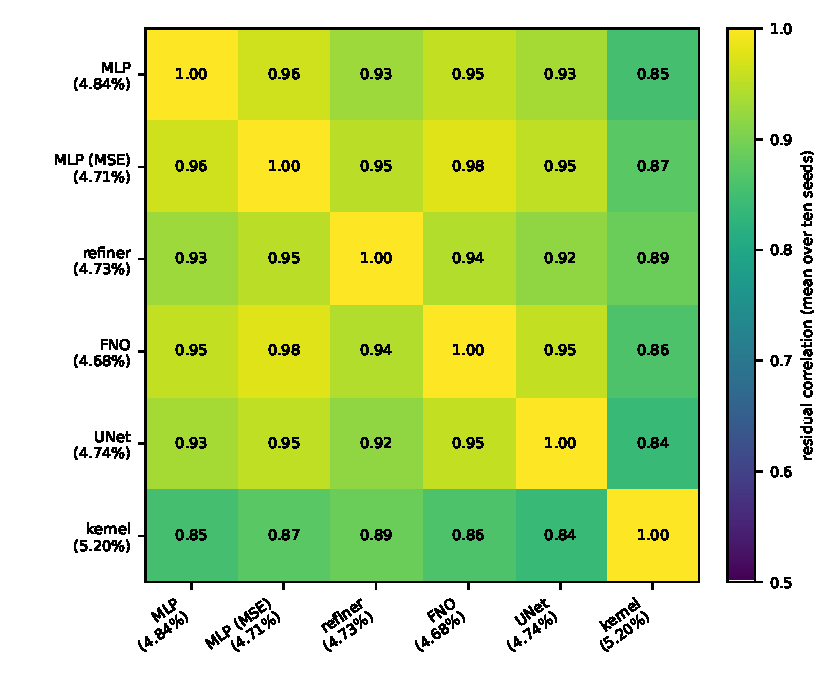
\includegraphics[width=0.62\linewidth]{figs/corr.pdf}
\caption{Centered correlation of per-sample normalized residuals on the validation
split, six members, averaged over the ten seeds of the second experiment.
Across seeds and pairs the entries range between $0.82$ and $0.98$.
The mean over pairs is $0.919\pm0.005$ across seeds; the kernel predictor
has correlation \corrKerLo--\corrKerHi{} with the normalized-MSE network
at every seed. These centered correlations differ from the uncentered
alignments summarized in Section~\ref{sec:diversity}.}
\label{fig:corr}
\end{figure}

\begin{figure}[t]
\centering
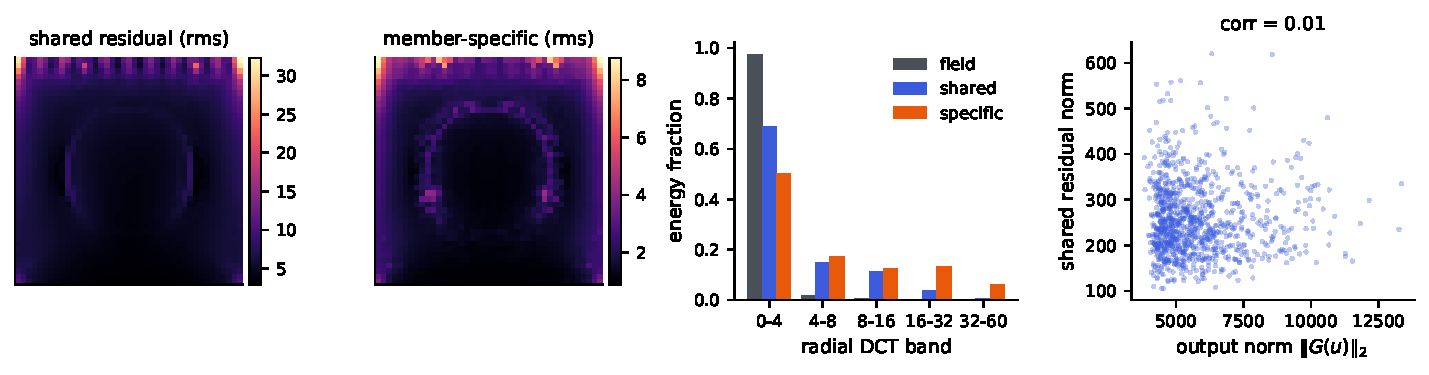
\includegraphics[width=\linewidth]{figs/shared.pdf}
\caption{Spatial and spectral structure of the shared residual $c$ (across-member mean of the
residual fields), at one seed. Left to right: rms of $c$ over the grid; rms of
the member-specific remainders; radial DCT band energies of the stress fields,
of $c$, and of the member-specific remainders; and the norm of $c$ against the output norm,
whose correlation is $0.01$.}
\label{fig:shared}
\end{figure}


\subsection{Spectra and effective dimension}
\label{sec:spectra}
A separate diagnostic uses $6000$ rows sampled
without replacement from the $19000$ training rows. The load coordinates are
standardized using the full training design. The Mat\'ern-$5/2$ length scale
is fixed at four times the median distance on a $2000$-row training subsample,
and the marked nugget is $10^{-5}$. These fixed diagnostic parameters need
not match those selected by each deployed correction. The split and sampling
generators both use seed~0.

The effective dimension is $d_{\mathrm{eff}}(10^{-5})=103.11885$,
where each eigenvalue $\mu_i$ contributes $\mu_i/(\mu_i+6000\lambda)$.
The Cholesky calculation of
$6000-6000\lambda\operatorname{tr}\big((K_S+6000\lambda I)^{-1}\big)$ agrees with the
eigenvalue sum to $1.7\times10^{-11}$. This calculation describes the
subsample smoother rather than the full $19000$-row fit. Low effective dimension does
not reduce the cubic work of the dense factorization used here.


\subsection{Computation and memory}
\label{sec:cost}
The structural-mechanics experiments use cloud CPU instances and dense,
exact linear solves for the kernel stages. At the experimental
dimensions, an eight-thread timing calculation measured $\costGramS$ seconds to
build a $19000\times19000$ Gram matrix in blocks, $\costCholS$ seconds for its
Cholesky factorization, and $\costSolveS$ seconds to solve for 1681 output
coordinates. The roughly one-minute total excludes hyperparameter search,
network training and prediction. Values in this timing experiment are
synthetic; the dimensions and operations match the experiment. The factorization
performs $n^3/3\approx2.3\times10^{12}$ floating-point operations. No GPU, inducing points, preconditioner or
stochastic linear solver is used in the correction.

Gram-matrix construction is the principal memory constraint at this size.
Forming a full squared-distance matrix and its
elementwise transforms allocates several $2.9$\,GB temporaries at once;
in the experiments this construction required more than the available
memory on a $31$\,GB instance. The block-filled timing
diagnostic has a measured peak of $\costPeakBlockGb$\,GiB, including the
factorization and solves, compared with $\costPeakNaiveGb$\,GiB after the
full-matrix construction. The reported pipeline uses full-size temporaries; the lower peak belongs
to the separate block-filled implementation. The neural means have a few million parameters and include both metric-loss
and normalized-MSE training. Splits are specified by permutation seeds and
inputs are the 41-dimensional loads described in Section~\ref{sec:benchmark}.

\subsection{Uncertainty quantification}
Theorem~\ref{thm:or} gives a conditional bound for a residual function in the
kernel native space with consistent training labels. The deployed correction
uses mixed training predictions: the kernel channel is constructed with
foldwise fits whose target centering uses the pooled training labels, while
neural predictions on these rows are in-sample. These labels need not equal
$G(X)-m_{\mathrm{full}}(X)$ for the deployed mean. The theorem applies to the deployed error under its stated consistency
and native-space assumptions and, where applicable, the mismatch term.

Table~\ref{tab:norms} reports a computable diagnostic: the squared RKHS norms
of ridge functions fitted to the two label arrays. With the selected
correction kernel at seed $0$, the residual-label fit has a norm about
\normRatio$\times$ smaller than the raw-stress fit and about
\normRatioNorm$\times$ smaller per unit label energy. These ratios depend on
the nugget and the scale. The mixed residual labels prevent identifying this
fitted norm with a lower bound for the native-space norm of the deployed
residual $G-m_{\mathrm{full}}$.

The design factor $P_\lambda$ correlates weakly with the deployed surrogate's
absolute error (Pearson \uqCorrAbs) and negatively with relative error. Its
correlation with the output norm is \uqCorrNorm{} (Figure~\ref{fig:uq}), so
its association with error depends on normalization by output amplitude.
Ensemble disagreement has correlation
$\uqDisAbs\pm0.006$ with absolute error across ten seeds and
$-0.25\pm0.04$ with relative error. The corresponding four-member absolute
error correlation is \uqDisAbsFour. Thus neither signal ranks the
remaining error well. A spread statistic is insensitive to a common additive
error shared by all members, which is consistent with the residual alignment
observed here.

Three bands are calibrated on $1000$ cases selected from the test block and
scored on the other $19000$: the scores are $\|e\|_2/P_\lambda$, $\|e\|_2$
(constant radius), and $\|e\|_2$ divided by ensemble disagreement. Each seed's
$P_\lambda$ uses its own selected correction kernel and training design.
The measured coverages are split diagnostics on the public test block. The marginal split-conformal theorem applies when the
predictor and score are fixed independently of exchangeable calibration and
future observations; the exact Beta and Beta--binomial descriptions additionally
require conditionally i.i.d. continuous scores (or an appropriate randomized
rank construction). A random partition of a fixed benchmark pool alone does not supply these
sampling assumptions.

For the six-member pipeline the $P_\lambda$ band has empirical coverage
$\uqPlamSix\pm\uqPlamSixSd\%$ at the nominal \uqCoverNom\% level and
$\uqPlamSixHi\pm\uqPlamSixHiSd\%$ at $95\%$. Under the i.i.d.-continuous
reference model, $m=1000$ gives latent coverage
$\mathrm{Beta}(901,100)$ at the $90\%$ level; with $19000$ independent
evaluation scores its central $95\%$ Beta--binomial reference interval is
$[88.0\%,91.8\%]$. At nominal $95\%$ coverage, the corresponding central
$95\%$ reference interval is $[93.5\%,96.3\%]$.
All ten six-member coverages fall inside these intervals at each
level.

The constant-radius band covers $\uqRawSix\pm\uqRawSixSd\%$ and
$\uqRawSixHi\pm\uqRawSixHiSd\%$, inside the reference intervals at ten of
ten seeds at both levels; the $P_\lambda$ band is on average
\uqWidthRatio{} times as wide. The disagreement-scaled band covers
$\uqDisSix\pm\uqDisSixSd\%$ and $\uqDisSixHi\pm\uqDisSixHiSd\%$, with
one seed on the upper edge of the $95\%$ reference interval. The five-member
pipeline gives $\uqPlamFive\pm\uqPlamFiveSd\%$ and
$\uqPlamFiveHi\pm\uqPlamFiveHiSd\%$ for the $P_\lambda$ band (ten and nine
seeds inside), and $\uqRawFive\pm\uqRawFiveSd\%$ and
$\uqRawFiveHi\pm\uqRawFiveHiSd\%$ for the constant-radius band (ten inside
at both levels). The constant-radius band is narrower, and the kernel design factor
provides no measured efficiency gain.

\begin{table}[t]
\centering
\caption{Fitted-norm diagnostic of the residual correction at seed $0$ of the
complete-schedule experiment: the same validated correction kernel (scale
multiplier $2$, nugget $10^{-3}$, median length scale) ridge-fitted to the
raw stress fields and to the six-member stack residuals on the training
split. $\|\widehat r\|_K^2=\operatorname{tr}(\alpha^\top K\alpha)$ is the
squared RKHS norm of the fitted function; the last column divides it by
the energy of the fitted label array. The residual labels mix foldwise
kernel predictions and in-sample neural predictions, so these numbers are
not identified as lower bounds for the native-space norm of the deployed
residual. The ratios depend on the selected nugget and scale. Much of the raw
ratio reflects output amplitude: per unit energy the
residual's fitted norm is \normRatioNorm{} times smaller at this seed, not
\normRatio{}; at seeds $1$ and $2$, whose corrections chose scale
multipliers $1$ and $2$, the raw ratios are \normRatioLo{} and $4300$ and the
normalized ones \normRatioNormLo{} and $7.6$. }
\label{tab:norms}
\begin{adjustbox}{max width=\linewidth}
\begin{tabular}{lccc}
\toprule
Kernel regresses & $\|\widehat r\|_K^2$ & energy $\|T\|_F^2$ & $\|\widehat r\|_K^2/\|T\|_F^2$ \\
\midrule
Raw stress fields ($m=0$) & $7.12\times10^{8}$ & $6.77\times10^{11}$ & $1.05\times10^{-3}$ \\
Ensemble residuals & $1.45\times10^{5}$ & $1.21\times10^{9}$ & $1.20\times10^{-4}$ \\
\midrule
Ratio & \normRatio$\times$ & \normEnergyRatio$\times$ & \normRatioNorm$\times$ \\
\bottomrule
\end{tabular}
\end{adjustbox}
\end{table}

\begin{figure}[t]
\centering
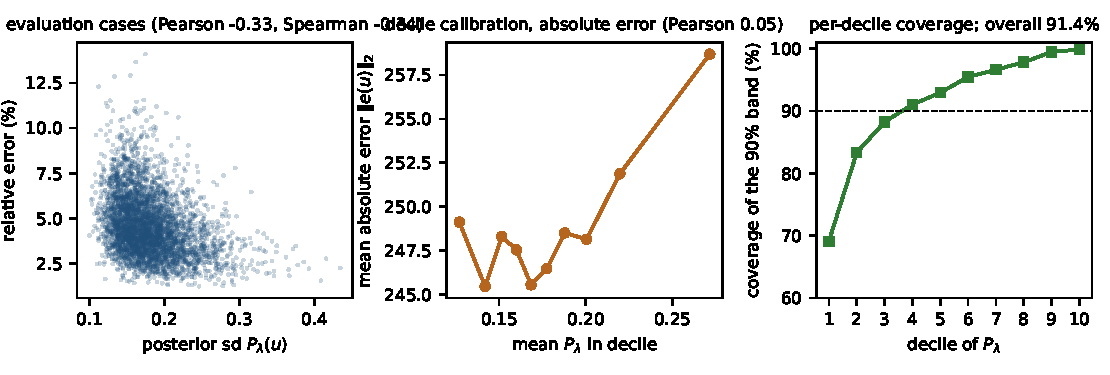
\includegraphics[width=\linewidth]{figs/uq.pdf}
\caption{Uncertainty measures for the six-member correction at seed 0.
Calibration uses $1000$ test-block cases and evaluation uses the other
$19000$, as in Section~\ref{sec:uq}. Left: the Gaussian process
posterior standard deviation $P_\lambda$ against relative error; the
association is negative (Pearson $-0.33$) because large-amplitude outputs have
small relative error. Middle: decile calibration of $P_\lambda$ against
absolute error $\|e(u)\|_2$; the
association is weak (Pearson $0.05$). Right: coverage of the
$P_\lambda$-scaled $90\%$ band within each decile of $P_\lambda$: $91.4\%$
overall, but from $69\%$ in the lowest decile to $99.9\%$ in the highest,
so coverage varies strongly with the design factor despite an overall
value close to the nominal level. Across the ten seeds the same band
has coverage $\uqPlamSix\pm\uqPlamSixSd\%$ at the nominal \uqCoverNom\% level,
inside the i.i.d.-continuous Beta--binomial reference interval at ten
seeds of ten; the constant-radius band
is the narrower of the two (Section~\ref{sec:uq}).}
\label{fig:uq}
\end{figure}

\begin{figure}[t]
\centering
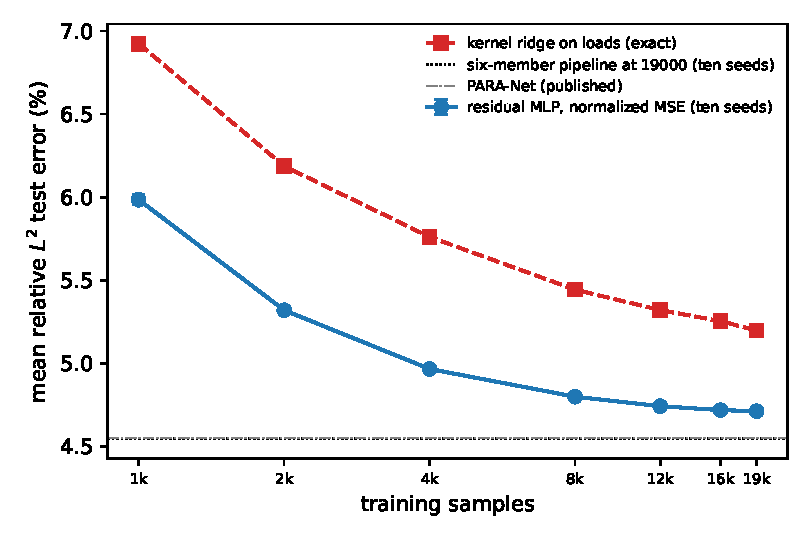
\includegraphics[width=\linewidth]{figs/curve_seeded.pdf}
\caption{Structural-mechanics learning curves. The first
$N+1000$ rows of the training pool are used, with the final $1000$ reserved
for validation and the first $N$ for fitting. The validation split is fixed
across seeds at each $N$ and changes with $N$; evaluation uses the full test
block. The curves give mean relative test error for the normalized-MSE
network (mean and standard deviation over ten seeds) and deterministic
Mat\'ern kernel ridge on loads, with both axes logarithmic. The horizontal lines mark the six-member pipeline at $19000$
samples and the quoted PARA-Net result. Error bars are smaller than the
markers above $4000$.}
\label{fig:scaling}
\end{figure}


\subsection{Seed variation and test-sample uncertainty}

The seed standard deviations describe variation from initialization and
selection on a common fixed test block. They do not include the
sampling uncertainty of a future evaluation set. If cases were independent
and representative of a target population, the reported per-case standard
deviation $0.0169$ would give a mean-error standard error of $\seTest$
percentage points over $20000$ cases.

The published baselines do not provide per-case predictions or comparable
training replicates. Their differences from our scores therefore do not
support a paired significance test or an equivalence conclusion. Combining
two copies of our sampling term in quadrature gives approximately
$\seUnpaired$ points, but this imputes an unknown baseline variance and
covariance structure. It is a sensitivity calculation. The $0.098$-point difference from PCA-Net
and $0.022$-point difference from PARA-Net for the five-member pipeline are
benchmark-score differences whose statistical uncertainty cannot be
determined from the available baseline summaries.

Within the two experiments, per-case paired differences isolate changes
between fitted predictors on the same cases. The full pipeline reduces error by
$\errEndToEnd$ percentage points, and removing the FNO increases it by
$\fnoGain\pm\fnoGainSd$ points across ten seeds, with the latter direction
holding at all ten.

The validation second-moment simplex optimum distributes weight among the
five members: refiner $0.31\pm0.04$, FNO $0.34\pm0.06$, normalized-MSE network
$0.24\pm0.08$, kernel $0.06\pm0.03$, and metric-trained MLP $0.06\pm0.04$.
The kernel has nonzero weight at all ten seeds and the metric-trained MLP at
nine. For the six-member experiment the corresponding shares are UNet
$0.32\pm0.06$, FNO $0.30\pm0.07$, refiner $0.27\pm0.04$, kernel
$0.06\pm0.02$, normalized-MSE network $0.03\pm0.04$, and metric-trained MLP
$0.02\pm0.02$. The FNO's large share despite its single-member ranking
illustrates the role of off-diagonal residual second moments.

Proposition~\ref{prop:secmom}(i) uses the uncentered alignment
$S_{12}/\sqrt{S_{11}S_{22}}$. The descriptive centered correlations in
Figure~\ref{fig:corr} need not equal this alignment. Exact convex-mixture
calculations use the uncentered second-moment matrix, rather than the
centered-correlation summaries.

The completed FNO schedule reduces its validation RMS error from $\fnoRmsA\%$ to
$\fnoRmsB\%$, while its descriptive correlation with the normalized-MSE
network increases from $\corrFnoLo$--$\corrFnoHi$ to $0.974$--$0.980$.
The five-member validation quadratic optimum is $\predRMS\%$ before
and $\predRMSFiveC\%$ after this change. These measured changes are consistent with an accuracy
improvement being offset by greater residual alignment.
Proposition~\ref{prop:exchange} gives a local sensitivity calculation for
fixed positive RMS errors and uncentered alignment; the centered-correlation
summaries do not determine that sensitivity.

For an exactly equicorrelated equal-error family,
Proposition~\ref{prop:secmom}(ii) gives the limiting RMS value
$\bar e\sqrt{\bar\varrho}$. Substituting the measured mean RMS error gives
the heuristic value $\ensFloor\pm\ensFloorSd\%$ for five members using
the mean centered correlation, and $\ensFloorSix\pm\ensFloorSixSd\%$
for six members using the mean uncentered alignment. The empirical pools are heterogeneous,
so these substitutions are heuristic diagnostics. The
one-sided entrywise bounds below and the sixty-member bound use the actual
uncentered second-moment matrices instead.

All these bounds concern RMS error $\mathcal E_2$ for global convex weights.
Jensen's inequality gives $\mathcal E_1\le\mathcal E_2$ for the same
predictor, so an RMS lower bound does not transfer to mean error. The deployed
pipeline's per-pixel affine weights and kernel correction also place it
outside the global convex class. Among global sum-to-one weights the signed
and convex optima differ by at most $0.00052$ percentage points across the fitted pools, but they do not always coincide: the signed minimizer has a negative
coordinate at seven six-member seeds and one five-member seed.

The selected input-space residual correction improves the five-member stack
by $\corrGain$ points at $n=19000$. Figure~\ref{fig:scaling}
reports the observed response to sample size: the normalized-MSE network
goes from $\lcMlpOneK\pm\lcMlpOneKSd\%$ at $N=1000$ to
$\lcMlpEightK\pm\lcMlpEightKSd\%$ at $8000$ and
$\lcMlpNineteenK\pm\lcMlpNineteenKSd\%$ at $19000$; the kernel goes from
$\lcKrrOneK\%$ to $\lcKrrEightK\%$ and $\lcKrrNineteenK\%$.
Over the measured range above $8000$, fitted log-log slopes are
$-\lcSlopeMlp\pm\lcSlopeMlpSd$ for the network and $-\lcSlopeKrr$ for the
kernel. The final increase in sample size reduces error by
$\lcLastGain\pm\lcLastGainSd$ percentage points, with a reduction at
nine seeds. The last two increases together reduce error by
$\lcLastTwoGain\pm\lcLastTwoGainSd$ percentage points, with a reduction
at all ten seeds. These are finite-range fits.
A three-parameter fit $e_\infty+cN^{-\alpha}$ gives different extrapolated
asymptotes, $4.64\%$ and $4.88\%$, so it does not locate a common floor.
Shared
approximation bias and target discretization artifacts remain unresolved
explanations for the residual plateau.

On the five-member test set, Corollary~\ref{cor:floorpinch} gives a
normalized bracket $[0.949\pm0.005,1.039\pm0.004]$ and fitted-global-stack
quadratic risk $0.980\pm0.003$. That risk uses the deployed global weights. The six-member validation-matrix
calculation reports a bracket $[0.933\pm0.007,1.032\pm0.004]$ and normalized
simplex optimum $0.972\pm0.005$. The corollary upper-bounds the minimum by
the uniform-weight risk; an arbitrary fitted ensemble need not lie below
that upper bound, although the five-member weights do.

From the six-member validation matrices, the one-sided
RMS floor $\sqrt{\min_{i\ne j}S_{ij}}$ is $4.820\pm0.062\%$, the stronger
finite-six-member lower bound is $4.849\pm0.060\%$, and the quadratic
optimum is $\predRMSSix\pm\predRMSSixSd\%$. The dispersion factors
$\dispFac\pm\dispFacSd$ and $\dispFacSix\pm\dispFacSixSd$ compare
$\mathcal E_1$ and $\mathcal E_2$ on the same validation data used to compute
the weights. They measure the difference between the two metrics on those validation data. For six members the ratio of test mean error to validation RMS
error is $0.9357\pm0.0110$; that ratio additionally includes transfer between
samples and is not a pure dispersion factor.

\paragraph{The sixty-predictor pool.} The analysis of
Section~\ref{sec:seeds-arch} uses the test predictions of all sixty
members in the second experiment. A fixed permutation divides
the test block into $1000$ fitting and $19000$ evaluation cases for this
pooling exercise. Convex weights fitted on the first subset
are evaluated on the second; the hindsight optimum is explicitly optimized
on the evaluation matrix. Equal-weight seed curves average over all subsets
for RMS error; mean errors use all subsets where there are at most $45$, and
$40$ random subsets otherwise.

Using the evaluation matrix, the smallest diagonal is $0.0024512070$ and the
within- and between-architecture lower second moments divided by that
diagonal are $0.9807963$ and $0.9377968$. Theorem~\ref{thm:blockfloor} then
gives $\saBound\%$, below the hindsight RMS optimum
$\saSixtyOracleRms\%$. This empirical lower bound applies to global convex combinations of these
sixty predictors on the evaluation cases.
An extension to more seeds would require the same entrywise lower bounds to
hold for those additional members.

Within the existing ten-seed blocks, square roots of the smallest
within-architecture second moments are approximately $4.93\%$ for the FNO,
$4.96\%$ for the normalized-MSE network, $4.97\%$ for the refiner,
$4.94\%$ for the UNet, $4.90\%$ for the metric-loss MLP and $5.46\%$ for
the kernel. The corresponding ten-seed equal-weight errors lie close to
these empirical references. Replacing lower moments by mean moments in the block formula
returns the uniform sixty-member mixture's value exactly, as an algebraic identity.

At the pipeline's fixed ridge, per-pixel affine fitting on all sixty members
has evaluation error $\saPerpixSixty\%$, versus $\saPerpixMeans\%$ for the
six ten-seed means and $\saPerpixSeedZero\%$ for six members at seed~0.
The leave-one-out ridge comparisons in Section~\ref{sec:seeds-arch} show that
this difference depends on regularization. Removing the UNet seeds changes the
uniform-weight mean error from $\saSixtyEq\%$ to $\saFiftyEq\%$.

For the first experiment the test-error seed standard deviation is $0.005$
points at uniform weights, $0.006$ for fitted global weights,
$\errStackSd$ for the affine stack and $\errPipeSd$ after correction.

\begin{figure}[t]
\centering
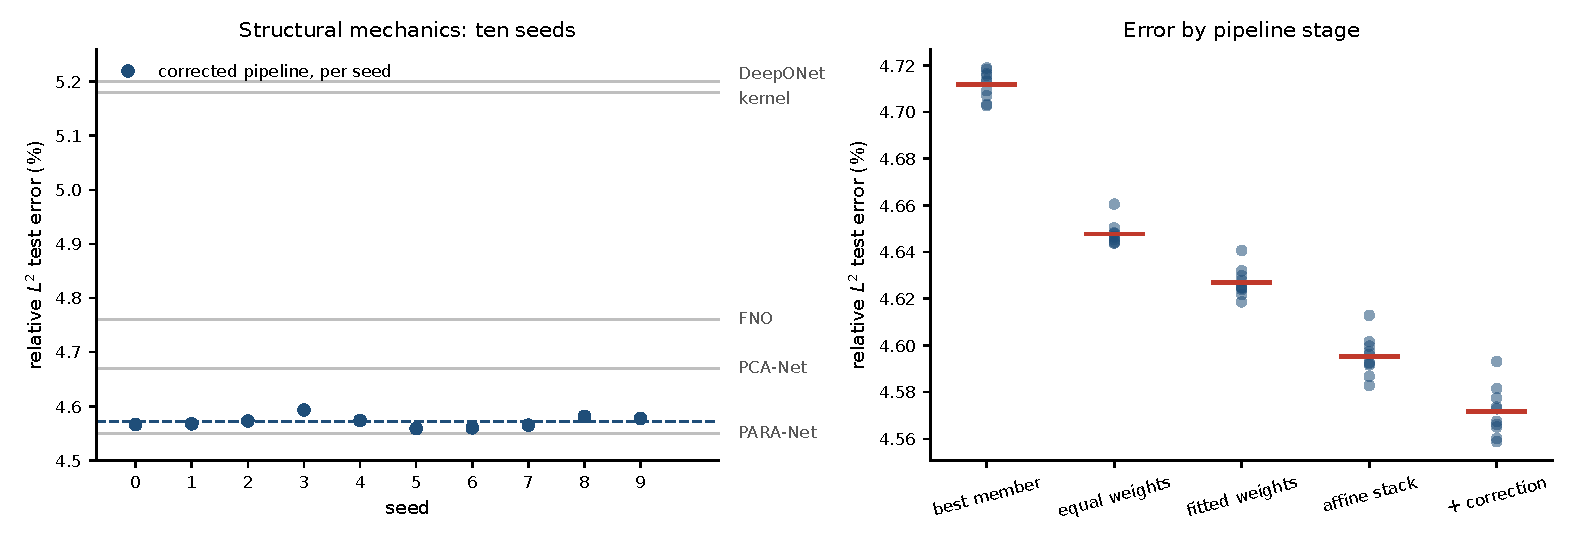
\includegraphics[width=\linewidth]{figs/seedspread.pdf}
\caption{Left: the corrected pipeline's test error at each of the ten seeds
(points), their mean (dashed), and the five published benchmark errors on the
same axis (grey). These show the variability of our pipeline;
comparable seed distributions are unavailable for the published methods. Right: test error at successive pipeline stages for each seed, with the
stage means marked. Fitting per-pixel weights lowers the
mean; seed spreads at each stage are reported in the text.}
\label{fig:seedspread}
\end{figure}


\section{OCO-2 input metrics and data scaling}
\label{supp:oco2}
\subsection{Input rescaling and prediction error}
Both raw-input kernels are fitted at five nested
training sizes over a sixteenfold range, at ten seeds on each band.
Each sensitivity map is estimated from the training rows available at its
own sample size using the standardized-input least-squares matrix $A$ in
Supplement~\ref{supp:oco-input}. Rank summaries use the separate matrix
$B=X_{\rm tr}^{\dagger}Z$ in the released input coordinates on all 18000
fitting rows. The singular-value counts retaining $99\%$ of $B$'s squared
energy are $12/20$, $14/24$ and $13/24$; the corresponding participation
ratios $(\sum_j\sigma_j)^2/\sum_j\sigma_j^2$ are $11.99$, $13.63$ and
$13.33$. These describe the fitted linear maps in those coordinates.

Table~\ref{tab:aniso} reports finite-range log--log slopes. On O2 the paired
slope difference is small relative to its seed variation. The adapted
kernel's fitted exponent is larger on the two CO$_2$ bands, by $0.011$ and
$0.052$. At $n=18000$ the isotropic-to-adapted error ratios are
$1.353\pm0.008$, $1.118\pm0.002$ and $1.514\pm0.114$. Thus the tested
rescaling improves prediction at that training size but leaves much of
the error difference between raw-input and feature kernels. These finite-range slopes are distinct from the rank-truncation bound of
Proposition~\ref{prop:aniso}, which requires Lipschitz, domain-radius, and
native-space assumptions beyond the estimated ranks.

\begin{table}[t]
\centering
\caption{The raw-input kernel refit at nested training sizes, ten seeds per
band. ``Rank'' counts singular values of the fitting-set matrix $B=X_{\rm tr}^{\dagger}Z$
holding $99\%$ of the squared energy, out of the input dimension. The exponent
difference is paired within seed; its standard deviation is over seeds. The
last column is the isotropic-to-adapted error ratio at $n=18000$.
The slopes are descriptive fits over the finite sizes tested.}
\label{tab:aniso}
\begin{adjustbox}{max width=\linewidth}
\begin{tabular}{lccccc}
\toprule
Band & Rank & $-$slope iso & $-$slope adapted & difference & ratio at $n{=}18000$ \\
\midrule
O2         & 12/20 & $0.221\pm0.007$ & $0.215\pm0.017$ & $+0.006\pm0.015$ & $1.353\pm0.008$ \\
weak CO$_2$   & 14/24 & $0.086\pm0.005$ & $0.097\pm0.006$ & $-0.011\pm0.009$ & $1.118\pm0.002$ \\
strong CO$_2$ & 13/24 & $0.203\pm0.029$ & $0.255\pm0.020$ & $-0.052\pm0.021$ & $1.514\pm0.114$ \\
\bottomrule
\end{tabular}
\end{adjustbox}
\end{table}

At $n=18000$, the sweep and Table~\ref{tab:oco2} use the same tuning
routine and standardized inputs and give identical raw-kernel results and
selected hyperparameters at every seed.
Training duration affects the comparison: a separate single-seed
$750$-epoch O2 run reaches $3.82\%$ (flat network)
and $3.71\%$ (feature head), with the combination at $3.71\%$ reduced and $0.0174\%$
radiance. The $250$-epoch comparison is therefore sensitive to training
duration and does not establish convergence.

The training-loss comparison further distinguishes coordinate
weighting from per-case weighting. The second network in
Table~\ref{tab:oco2} is trained on a diagonally weighted loss over the
reduced coefficients, $\|s_z\odot(\hat z-z)\|/\|s_z\odot z\|$. That is a surrogate for the radiance-relative error: the reported radiance metric maps predictions through the stored PCA
reconstruction and divides by the reconstructed-radiance norm, and the
surrogate omits the reconstruction. The third network is trained in the
exact radiance metric, reconstruction and denominator included. Its
radiance error is higher than that of the surrogate-trained network:
$0.0571\pm0.0057\%$ against $0.0442\pm0.0044\%$ on O2
and $0.093\pm0.008\%$ against $0.075\pm0.003\%$ on SCO2, the surrogate having lower error at all ten seeds on both bands. The
ranking is reversed on WCO2 at eight of ten seeds
($0.064\pm0.015\%$ against $0.072\pm0.007\%$). The kernel heads built on
their features repeat the pattern. Tripling the training budget narrows the
O2 gap ($0.0212\%$ against $0.0201\%$ at $750$ epochs) without reversing it,
but these finite-budget comparisons do not identify why one training loss
performs better. By the reconstruction identity, the two losses share the
same numerator and differ in their target-dependent denominator, which
reweights cases. Both concentrate on the leading coefficients, while their
optimization and generalization behavior can differ. The coordinate
profile is consistent with this trade-off: the kernel-flow emulator
predicts the leading coefficient to $0.0012$ root mean square against the
flat network's $0.0054$, whereas the flat network is three to four times
more accurate on the trailing thirty coordinates. The relative errors depend on both the band and training budget.

The flat-network seeds permit a second-moment analysis similar to
that on structural mechanics.
For each band, the matrix $S$ contains the test-set second moments of the
normalized residuals of the ten flat-network seeds. Mixture risks are
measured in squared relative error, as in Proposition~\ref{prop:secmom}.

At uniform weights, $w^\top Sw$ and the
directly measured risk of the averaged prediction agree to $7\times10^{-18}$,
$3\times10^{-17}$ and $1\times10^{-17}$ on the three bands.

Over the $45$ seed pairs per band, the residual alignments are
$0.787\pm0.010$ (O2), $0.971\pm0.001$ (WCO2) and
$0.961\pm0.001$ (SCO2). An equicorrelation summary gives ten-member RMS
relative errors of $4.419\%$, $17.997\%$ and $9.267\%$, matching the
recorded uniform-mixture risks at the displayed precision. The corresponding
infinite-family values, $4.360\%$, $17.970\%$ and $9.248\%$, are
extrapolations under the equicorrelation model. They are not lower bounds
for untrained seeds or for the architecture class. The exact
finite-pool statement is the quadratic identity applied to the measured
matrix $S$.

Comparisons with another readout must use the same metric, since $S$
determines a squared-relative-error quantity and
Table~\ref{tab:oco2} reports the mean relative error $\mathbb E\,\ell$.
Measured in RMS relative error, the Mat\'ern head on learned
features reaches $4.575\%$, $18.11\%$ and $9.326\%$ --- better than an
individual seeded network ($4.915\%$, $18.238\%$, $9.433\%$) and worse than
that network's ten-seed ensemble. The ranking is the same in the mean metric,
where the seed ensemble reaches $3.916\%$ against the head's $4.111\%$ on
O2. The ten-network ensemble has lower error than the single feature-kernel
head in both metrics, but the predictors have different computational costs.

Lower residual alignment alone does not guarantee a useful mixture: the
weaker member's RMS error also enters Proposition~\ref{prop:secmom}(i).
An exploratory WCO2 Fourier-feature bandwidth sweep gives error near
$31\%$ with correlation $0.54$, and errors above $140\%$ with correlations
near $0.11$ (Figure~\ref{fig:floor}). The plotted errors and correlations
are rounded summaries; the admission-condition analysis in
Section~\ref{sec:secmom-margin} uses the exact uncentered second moments
of the eight-model pool.
Adding the exploratory architecture candidates
to coordinate selection changed the mean error by less than $0.01$
percentage points on each band.

\begin{figure}[t]
\centering
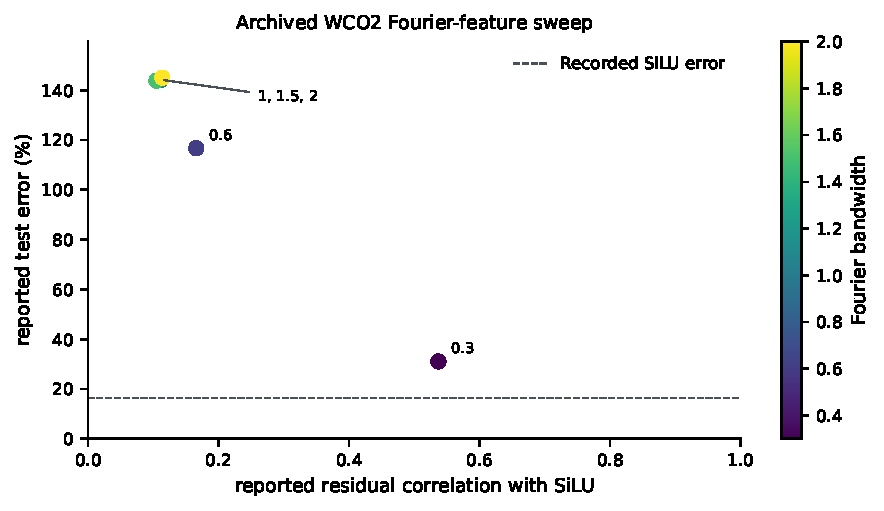
\includegraphics[width=\linewidth]{figs/floor.pdf}
\caption{Exploratory WCO2 Fourier-feature sweep. The legend identifies bandwidths; the
dashed line is the SiLU error of $16.37\%$. Three bandwidths nearly
coincide in the upper left. Errors and correlations are rounded
summaries of the exploratory measurements. The admission calculations in
Section~\ref{sec:secmom-margin} use exact uncentered second moments.}
\label{fig:floor}
\end{figure}

For the raw-input kernel against the flat network, the validation
summary has $\varrho=0.156$ and $e_n/e_k=0.157$, with RMS relative errors
$8.41\%$ and $53.5\%$. The sign of the criterion changes across seeds,
and the optimal mixture gains only a few ten-thousandths of a
percentage point. This explains the pair's small
contribution.

The combination chooses each coordinate from one of the three networks
and three feature-kernel heads using coordinatewise validation RMSE. By
Proposition~\ref{prop:percoord}, this minimizes an auxiliary separable
squared loss over that candidate product. Fixed sample denominators retain
separability for squared relative losses, with different sample weights
for the reduced and radiance criteria. The reported means of relative
norms instead couple coordinates through the square root. Consequently
this selector is not guaranteed to optimize either reported metric, or
both simultaneously. The same selected coordinates produce both reported
columns; the baseline emulator's predictions are not candidates.
Its seed-averaged errors are lower than those of the rescored
kernel-flow emulator in both criteria on all three bands: O2 reaches
$4.12\pm0.05\%$ against $16.89\%$ reduced and $0.0294\pm0.0020\%$ against
$0.0448\%$ radiance, SCO2 $8.08\pm0.01\%$ against $16.14\%$ and
$0.0584\pm0.0041\%$ against $0.1147\%$, and WCO2 $16.28\pm0.06\%$ against
$24.06\%$ and $0.0507\pm0.0052\%$ against $0.0599\%$. Counted by seed, the
combination has lower error than the emulator in both metrics at all ten
seeds on O2 and SCO2 and at nine of ten on WCO2. At the remaining WCO2 seed,
its radiance error is higher by $0.0015$ percentage points.

On O2 the combination's reduced mean is slightly worse than that of the
flat-feature head ($4.11510\%$ versus $4.11080\%$), while its radiance mean
improves from $0.07927\%$ to $0.02940\%$. The selector therefore improves radiance accuracy at a small cost in
reduced-coordinate accuracy. On WCO2, one seed has a radiance error
$0.0015$ percentage points higher than the source emulator. The paired-bootstrap interval for that seed is
$[-0.0012,0.0042]$ percentage points, while the other nine intervals are
negative. These are descriptive intervals on the public test cases.

\subsection{Learning curves and training budgets}
\label{sec:scaling}
The OCO-2 learning curve decreases more strongly with training
size than the structural-mechanics curve over the ranges examined.
The left panel of Figure~\ref{fig:ocoscaling} shows a one-seed O2 experiment
with a disjoint held-out set. A finite-range log--log fit gives slope
$-0.68$, with error decreasing from about $74\%$ at a few hundred pairs to
$4.3\%$ at $n=17700$. The main ten-seed combination at $18000$ training
pairs has mean $4.12\%$ at its $250$-epoch budget; the $3.71\%$ result
above belongs to a separate single-seed $750$-epoch experiment. These are
different protocols and should not be combined into one scaling fit.
The raw-input kernel improves more slowly over these sizes. The measured
curves do not identify the limiting source of error or an asymptotic
convergence rate.

The ClimSim experiments cover a larger data range. ClimSim \citep{yu2023climsim} is a climate emulation dataset of about
ten million samples that maps a $124$-dimensional atmospheric state to $128$
physics tendencies, with published neural baselines. The runs compare two model
families at one, two and three and a half million training samples.
Kernel hyperparameters are selected on a disjoint 2000-row validation
block drawn from the training pool. Each neural run retains the final
checkpoint of its 60-epoch schedule. Evaluation uses separate data; the
right panel of Figure~\ref{fig:ocoscaling} plots those points. Each experiment
seed draws its own $20000$-row test block, so the spreads below include that
variation.

For each output coordinate $j$, let
$v_j=N^{-1}\sum_{i=1}^N(y_{ij}-\bar y_j)^2+10^{-12}$ be its variance
on that seed's test block, and define
$J=\{j:v_j>10^{-6}\max_k v_k\}$. The reported score is the unweighted
mean of the coordinatewise coefficients of determination,
\[
 R^2=\frac{1}{|J|}\sum_{j\in J}
 \left(1-\frac{N^{-1}\sum_{i=1}^N(\hat y_{ij}-y_{ij})^2}{v_j}\right).
\]
The same active-coordinate set $J$ is used for both predictors at each seed.

The neural mean has higher $R^2$ than the kernel and improves with training
size: $0.544\pm0.005$ at one
million (five seeds), $0.563\pm0.004$ at two million and $0.575\pm0.004$ at
three and a half million (three seeds each). A published
multilayer-perceptron value near $0.6$ provides context; this comparison
does not use a matched split and scoring protocol. The corresponding kernel values are $0.390\pm0.007$, $0.391\pm0.006$ and $0.387\pm0.007$ at the three
sizes. Each kernel was fitted on a $6000$-row subsample, so the near-constant
error does not describe its response to increasing kernel training size.
A separate kernel-budget comparison uses the same protocol
(selection on the pool validation block, separate test evaluation, seed
$0$, the one-million slice): $\csCapSix$ at $6000$ rows, $\csCapTwelve$ at
$12000$ and $\csCapTwentyFour$ at $24000$ ($\csCapTwentyFourB$ at a second
seed, with a separately drawn test block). The $R^2$ value increases by about $0.03$ at the first budget doubling
and $0.01$ at the second, and at
$24000$ rows, the largest exact solve tested, its $R^2$ remains about $0.11$
below the network at
one million samples. The comparison remains unequal in training size and total computation:
the neural mean uses up to millions of examples, whereas the exact kernel
uses at most $24000$. The network has lower error under these budgets; matched-compute
comparisons and larger kernel fits remain untested. The reported range does not locate a
crossover between model families.

\begin{figure}[t]
\centering
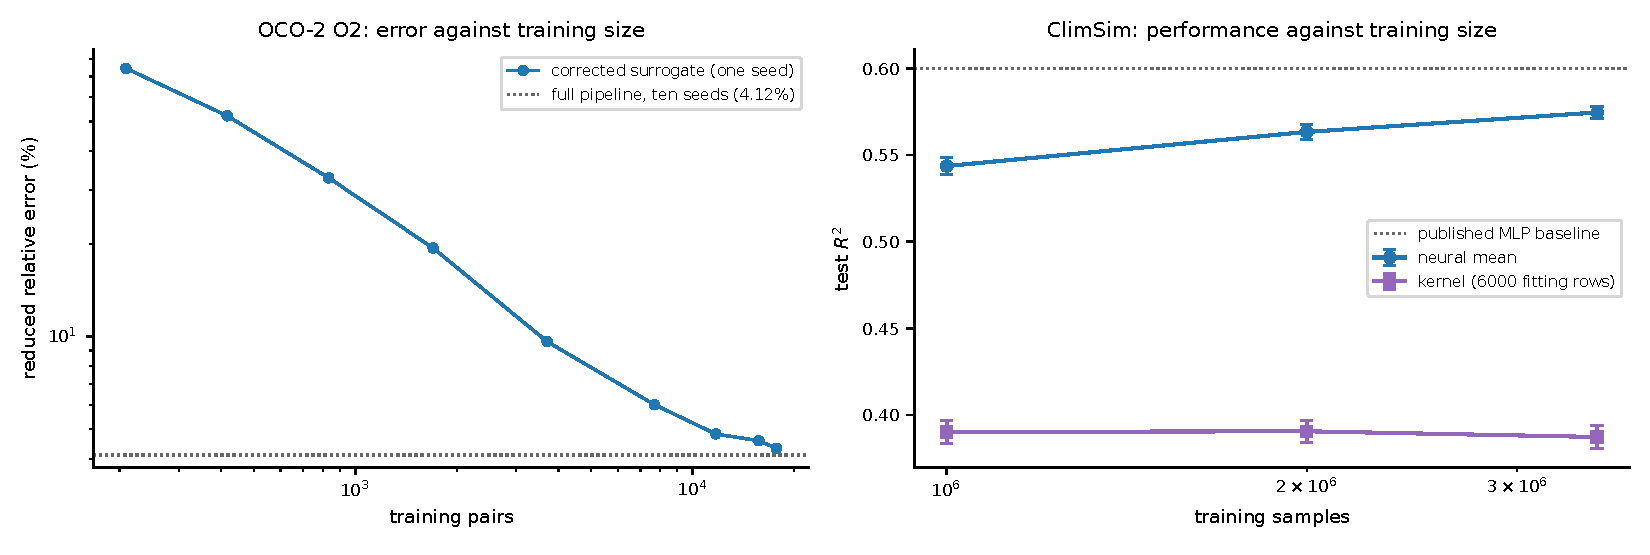
\includegraphics[width=\linewidth]{figs/scaling_seeded.pdf}
\caption{Error against training-set size. Left: the
OCO-2 O2 task, reduced error of the corrected surrogate at one seed, from the
data-scaling run; a finite-range log--log fit has slope $-0.68$, and the
error is $4.3\%$ at $n=17700$, against the
$4.12\%$ the ten-seed pipeline reaches on all $18000$ pairs (dotted). Right:
ClimSim, test $R^2$ over the active outputs defined in the text, at one,
two and three and a half million training samples --- five seeds at one million and three at each of the
larger sizes, error bars over seeds. No crossover between the two families is observed over this range. Each kernel is fitted on $6000$ rows, so its nearly constant error
across nominal training sizes reflects that fixed fitting budget. The separate
kernel-budget comparison is reported in the text. The neural
mean has higher $R^2$; the published baseline (dotted) is shown for orientation; the protocols are not matched.}
\label{fig:ocoscaling}
\end{figure}


\section{Proofs}
\label{app:proofs}
\subsection{Proof of Proposition~\ref{prop:sym}}
\label{proof:prop:sym}

By convexity of $\ell(\cdot,v)$,
\[
\ell\big(\widehat G_S(u),G(u)\big)\;\le\;\tfrac12\,\ell\big(\widehat
G(u),G(u)\big)+\tfrac12\,\ell\big(T\widehat G(Su),G(u)\big).
\]
Since $T$ is an involution, the equivariance $G(Su)=TG(u)$ applied at $u$
gives $TG(Su)=T^2G(u)=G(u)$, hence
\[
\ell\big(T\widehat G(Su),G(u)\big)=\ell\big(T\widehat G(Su),TG(Su)\big)
=\ell\big(\widehat G(Su),G(Su)\big),
\]
using the $T$-invariance of the loss. Taking expectations and using the
$S$-invariance of $\mu$ (so that $Su\sim\mu$ when $u\sim\mu$),
\[
\mathbb E\,\ell\big(\widehat G_S(u),G(u)\big)\le\tfrac12\,\mathbb
E\,\ell\big(\widehat G(u),G(u)\big)+\tfrac12\,\mathbb E\,\ell\big(\widehat
G(Su),G(Su)\big)=\mathbb E\,\ell\big(\widehat G(u),G(u)\big). \qed
\]

\subsection{Proof of Proposition~\ref{prop:kf}}
\label{proof:prop:kf}

Strict positive definiteness of the restricted kernel matrix makes $I_C$ the
(unique) interpolant of the pairs indexed by $C$, so $I_C(z_j)=v_j$ for $j\in
C$ and the terms of \eqref{eq:kf} indexed by $C$ vanish, which is the first
claim. For the second, write
\[
e_2(\theta;C)\;=\;\sum_{i\in B\setminus C} g(C,i),\qquad
g(C,i):=\|v_i-I_C(z_i)\|_2^2 .
\]
Conditionally on $C$, the sum has exactly $b/2$ terms, so
$e_2(\theta;C)=\tfrac b2\,\mathbb E_{i\sim\mathrm{Unif}(B\setminus C)}[g(C,i)]$,
and taking the expectation over $C$ proves the identity. The gradient claim
is immediate: for fixed $(B,C)$ the map $\theta\mapsto e_2(\theta;C)$ is
differentiable wherever the Cholesky factorization in $I_C$ is (the kernel
matrix stays positive definite in a neighborhood), and under a local
integrable Lipschitz bound the derivative passes under the expectation, so
$\mathbb E_{B,C}[\nabla_\theta e_2]=\nabla_\theta\,\mathbb E_{B,C}[e_2]$. \qed

\subsection{Proof of Proposition~\ref{prop:stack}}
\label{proof:prop:stack}

(i) Since $\sum_m w_m=1$,
$F_w(u)-G(u)=\sum_m w_m\,(f_m(u)-G(u))$, and the triangle inequality gives
$\|F_w(u)-G(u)\|_2\le\sum_m w_m\|f_m(u)-G(u)\|_2$. Dividing by $\|G(u)\|_2$
yields the pointwise claim; taking expectations gives the risk inequality, and
bounding each $\ell(f_m(u),G(u))$ by $B$ gives $\ell(F_w(u),G(u))\le B$.

(ii) For $M=1$ there is no weight selection and the asserted inequality
is immediate. Suppose $M\ge2$ and write $\ell_u(w)=\ell(F_w(u),G(u))$. First, $\ell_u$ is Lipschitz on
$\Delta$ for the $\ell^1$ norm: for $w,w'\in\Delta$, the reverse triangle
inequality and the argument of (i) give
\[
|\ell_u(w)-\ell_u(w')|\;\le\;\frac{\big\|\sum_m (w_m-w'_m)(f_m(u)-G(u))\big\|_2}
{\|G(u)\|_2}\;\le\;B\,\|w-w'\|_1 .
\]
Next, discretize the simplex. For $k\in\mathbb N$ let
$\mathcal G_k=\{w\in\Delta:\,kw\in\mathbb Z^M\}$; its cardinality is the number
of compositions of $k$ into $M$ nonnegative parts,
$\binom{k+M-1}{M-1}\le (k+1)^{M-1}$. Given $w\in\Delta$, set
$w'_i=\lfloor kw_i\rfloor/k$ for $i<M$ and $w'_M=1-\sum_{i<M}w'_i$; then
$w'\in\mathcal G_k$ (the last coordinate is a multiple of $1/k$ and is
$\ge w_M\ge0$ because the first $M-1$ coordinates only decreased), and
\[
\|w-w'\|_1=\sum_{i<M}(w_i-w'_i)+\big(w'_M-w_M\big)
=2\sum_{i<M}(w_i-w'_i)\;\le\;\frac{2(M-1)}{k}.
\]
By (i) the per-sample loss lies in $[0,B]$, so for each fixed $w'$ Hoeffding's
inequality gives
$\mathbb P\big(|\widehat R(w')-R(w')|>t\big)\le2e^{-2mt^2/B^2}$, and a union
bound over $\mathcal G_k$ shows that with probability at least $1-\delta$,
\[
\sup_{w'\in\mathcal G_k}\big|\widehat R(w')-R(w')\big|\;\le\;
B\sqrt{\frac{\log\!\big(2|\mathcal G_k|/\delta\big)}{2m}} .
\]
On this event, for every $w\in\Delta$, approximating by its grid point and
using the Lipschitz property for both $R$ and $\widehat R$,
\[
\big|\widehat R(w)-R(w)\big|\;\le\;
B\sqrt{\frac{\log(2|\mathcal G_k|/\delta)}{2m}}+\frac{4B(M-1)}{k}.
\]
If $w^\star$ minimizes $R$ over $\Delta$, the empirical minimizer satisfies
$R(F_{\widehat w})\le\widehat R(\widehat w)+\sup_\Delta|\widehat R-R|
\le\widehat R(w^\star)+\sup_\Delta|\widehat R-R|
\le R(F_{w^\star})+2\sup_\Delta|\widehat R-R|$. Choosing $k=m(M-1)$ and using
$|\mathcal G_k|\le(m(M-1)+1)^{M-1}$ gives
\[
R(F_{\widehat w})\;\le\;\min_{w\in\Delta}R(F_w)+\frac{8B}{m}
+B\sqrt{\frac{2\big((M-1)\log(m(M-1)+1)+\log(2/\delta)\big)}{m}} ,
\]
which is the claim. \qed

\subsection{Proof of Lemma~\ref{lem:select}}
\label{proof:lem:select}

For each $k$ the validation scores $\ell(g_k(\tilde u_i),G(\tilde u_i))$,
$i\le m'$, are i.i.d., take values in $[0,B]$, and have mean $R(g_k)$; the
maps $g_k$ are fixed relative to this sample, which is the only place the
independence assumption enters. Hoeffding's inequality gives, for each $k$,
\[
\Pr\Big(\big|\widehat R(g_k)-R(g_k)\big|\ge t\Big)\;\le\;
2\exp\!\big(-2m't^2/B^2\big),
\]
so with $t=B\sqrt{\log(2K/\delta)/(2m')}$ and a union bound over $k\le K$,
all $K$ deviations are below $t$ simultaneously with probability at least
$1-\delta$. On that event, if $k^\ast$ attains $\min_k R(g_k)$,
\[
R(g_{\widehat k})\;\le\;\widehat R(g_{\widehat k})+t\;\le\;
\widehat R(g_{k^\ast})+t\;\le\;R(g_{k^\ast})+2t,
\]
and $2t=B\sqrt{2\log(2K/\delta)/m'}$. \qed

\subsection{Proof of Proposition~\ref{prop:affine}}
\label{proof:prop:affine}

Fix a coordinate $j$ and abbreviate $\varphi=\varphi_j$, $Y(u)=G(u)_j$,
$D=\sqrt{M+1}$. Each entry of $\varphi(u)$ is bounded by $b$ in absolute
value (the members by assumption, the intercept entry by construction), so
$\|\varphi(u)\|_2\le bD$, and for $\|w\|_2\le W$ Cauchy--Schwarz gives
$|w^\top\varphi(u)|\le WbD$ and
$|w^\top\varphi(u)-Y(u)|\le b(1+WD)$. The losses
$\ell_w(u)=(w^\top\varphi(u)-Y(u))^2$ therefore take values in
$[0,L_\infty]$ with $L_\infty=b^2(1+WD)^2$.

\emph{Uniform deviation.} Consider the one-sided suprema
$Z^{+}=\sup_{\|w\|_2\le W}\big(\widehat R_j(w)-R_j(w)\big)$ and
$Z^{-}=\sup_{\|w\|_2\le W}\big(R_j(w)-\widehat R_j(w)\big)$ over the
validation sample of size $m$. Changing one sample moves either supremum by
at most $L_\infty/m$, so McDiarmid's inequality gives
$Z^{\pm}\le\mathbb E Z^{\pm}+L_\infty\sqrt{\log(4q/\delta)/(2m)}$, each with
probability at least $1-\delta/(2q)$. By
symmetrization, $\mathbb E Z^{\pm}\le 2\,\mathfrak R_m(\mathcal L)$, the
Rademacher complexity of the loss class. The loss is the composition of $t\mapsto t^2$,
restricted to $|t|\le b(1+WD)$ where it is $2b(1+WD)$-Lipschitz, with the
class $\{u\mapsto w^\top\varphi(u)-Y(u)\}$; translation by the fixed function
$Y$ leaves the Rademacher average unchanged (the translated term does not
involve $w$ and has zero mean), and for the linear class over the
$\ell^2$ ball,
\[
\mathfrak R_m\;\le\;\frac{W}{m}\,
\mathbb E\Big\|\sum_{i=1}^m\sigma_i\varphi(\tilde u_i)\Big\|_2\;\le\;
\frac{W}{m}\Big(\sum_{i=1}^m\mathbb E\|\varphi(\tilde u_i)\|_2^2\Big)^{1/2}
\;\le\;\frac{WbD}{\sqrt m},
\]
by Jensen's inequality. Talagrand's contraction lemma then gives
$\mathfrak R_m(\mathcal L)\le 2b(1+WD)\cdot WbD/\sqrt m$, hence
\[
Z^{\pm}\;\le\;\frac{4Wb^2D(1+WD)}{\sqrt m}
+L_\infty\sqrt{\frac{\log(4q/\delta)}{2m}}
\qquad\text{jointly with probability}\ge 1-\delta/q .
\]

\emph{Empirical risk minimization.} On this event, for any minimizer
$w^\ast$ of $R_j$ over the ball,
$R_j(\widehat w_j)\le\widehat R_j(\widehat w_j)+Z^{-}
\le\widehat R_j(w^\ast)+Z^{-}\le R_j(w^\ast)+Z^{+}+Z^{-}$, and
$Z^{+}+Z^{-}$ is bounded by the displayed excess. A union bound over the two
tails of each of the $q$ coordinates makes all events
hold simultaneously with probability at least $1-\delta$, and averaging over
$j$ preserves the (coordinate-uniform) bound. This proves (i).

For (ii), the ridge minimizer satisfies
$\widehat R_j(\widehat w_j)+\lambda\|\widehat w_j\|_2^2\le
\widehat R_j(w^\ast)+\lambda\|w^\ast\|_2^2$, so
$\widehat R_j(\widehat w_j)\le\widehat R_j(w^\ast)+\lambda\|w^\ast\|_2^2
\le\widehat R_j(w^\ast)+\lambda W^2$. Since by assumption
$\|\widehat w_j\|_2\le W$, the uniform event of part (i) applies to
$\widehat w_j$ and $w^\ast$ alike, and the chain above goes through with the
extra $\lambda W^2$. \qed

\subsection{Proof of Corollary~\ref{cor:floorpinch}}
\label{proof:cor:floorpinch}

The lower bound is Corollary~\ref{cor:floor}. For the upper bound, evaluate
the quadratic form at the uniform weights $w_m=1/M$:
\[
\frac{1}{\bar e^{\,2}}\,w^\top Sw
=\frac{1}{\bar e^{\,2}}\Big(\frac{1}{M^2}\sum_m S_{mm}
+\frac{1}{M^2}\sum_{m\neq k}S_{mk}\Big)
\;\le\;\frac{1+\delta_e}{M}
+\frac{M-1}{M}\,\big(\bar\varrho+\delta_\varrho\big),
\]
using the entrywise upper bounds and the counts $M$ and $M(M-1)$ of the two
sums. The right side equals
$\bar\varrho+\delta_\varrho+\big(1+\delta_e-\bar\varrho-\delta_\varrho\big)/M$,
and the minimum over the simplex is at most the value at any feasible point.
\qed

\subsection{Proof of Corollary~\ref{cor:certificate}}
\label{proof:cor:certificate}

Fix a coordinate $j$ and a grid point $\gamma$. Substituting the affine form
of the correction,
\[
h_{w,\gamma}(u)_j=w_j^\top\widetilde\varphi_{j,\gamma}(u)+o_{j,\gamma}(u),
\qquad
\widetilde\varphi_{j,\gamma}(u)=\varphi_j(u)-\Phi_j^\top c_\gamma(u),\quad
o_{j,\gamma}(u)=c_\gamma(u)^\top Y_j ,
\]
and neither $\widetilde\varphi_{j,\gamma}$ nor $o_{j,\gamma}$ depends on $w$
or on the validation sample: $c_\gamma$ is built from the training design
alone. Each component of $\Phi_j^\top c_\gamma(u)$ is a $c_\gamma$-weighted
sum of member values bounded by $b$, so its absolute value is at most
$b\,\|c_\gamma(u)\|_1\le b\kappa$, whence
$\|\widetilde\varphi_{j,\gamma}(u)\|_2\le bD+bD\kappa=bD(1+\kappa)$ and
$|o_{j,\gamma}(u)|\le b\kappa$. For $\|w\|_2\le W$ the prediction deviates
from the target by at most
$WbD(1+\kappa)+b\kappa+b\le b(1+WD)(1+\kappa)=:\tilde c$, so the squared
losses lie in $[0,\tilde c^{\,2}]$ and are $2\tilde c$-Lipschitz in the
prediction.

The argument of Proposition~\ref{prop:affine} now applies verbatim to the
class indexed by $w$ in the $W$-ball, for this fixed $(j,\gamma)$: the
Rademacher complexity of the affine part is at most
$W\,bD(1+\kappa)/\sqrt m$, contraction multiplies it by $2\tilde c$,
symmetrization doubles it, and McDiarmid at level $\delta/(2q|\Gamma|)$ adds
$\tilde c^{\,2}\sqrt{\log(4q|\Gamma|/\delta)/(2m)}$. A union bound over the
two tails of the $q|\Gamma|$ pairs makes, with probability at least
$1-\delta$, each one-sided deviation $Z^{\pm}_{j,\gamma}$, defined as in the
proof of Proposition~\ref{prop:affine},
at most
\[
\frac{4W b^2D(1+WD)(1+\kappa)^2}{\sqrt m}
+b^2(1+WD)^2(1+\kappa)^2\sqrt{\frac{\log(4q|\Gamma|/\delta)}{2m}} .
\]
On that event, write $\bar R(\gamma)=\tfrac1q\sum_jR_j(h_{\widehat w,\gamma})$
and $\widehat{\bar R}(\gamma)$ for its empirical version; averaging the
$Z_{j,\gamma}$ over $j$ bounds
$|\widehat{\bar R}(\gamma)-\bar R(\gamma)|$ by the same quantity for every
$\gamma$ simultaneously, including at the data-dependent $\widehat w$,
because the deviations are uniform over the ball. The selection chain
$\bar R(\widehat\gamma)\le\widehat{\bar R}(\widehat\gamma)+Z\le
\widehat{\bar R}(\gamma^\ast)+Z\le\bar R(\gamma^\ast)+2Z$ with
$\gamma^\ast$ the aggregate oracle then gives the display, whose constant is
$2Z$ in the factored form stated. When the $c_\gamma$ are kernel ridge
weights, Lemma~\ref{lem:kappa} supplies the hypothesis with
$\kappa=\kappa_{\mathrm{an}}$. \qed

\subsection{Proof of Lemma~\ref{lem:kappa}}
\label{proof:lem:kappa}

Fix $u$ and write $k_u=k(X,u)$, $t=n\lambda$, $A=K+tI$ and $c=A^{-1}k_u$.
Because $k$ is positive definite, the Gram matrix of the $n+1$ points
$u_1,\dots,u_n,u$ is positive semidefinite, and by the generalized Schur
complement this places $k_u$ in the range of $K$ with
$k_u^\top K^{+}k_u\le k(u,u)$, $K^{+}$ the pseudo-inverse. Diagonalize
$K=\sum_i\mu_iv_iv_i^\top$ and expand $k_u=\sum_i\beta_iv_i$ over the
eigenvectors with $\mu_i>0$; the Schur condition reads
$\sum_i\beta_i^2/\mu_i\le k(u,u)$. Then
\[
\|c\|_2^2=\sum_i\frac{\beta_i^2}{(\mu_i+t)^2}
=\sum_i\frac{\beta_i^2}{\mu_i}\cdot\frac{\mu_i}{(\mu_i+t)^2}
\;\le\;\frac{1}{4t}\sum_i\frac{\beta_i^2}{\mu_i}\;\le\;\frac{k(u,u)}{4t},
\]
because $(\mu+t)^2\ge4\mu t$ for all $\mu,t\ge0$. Cauchy--Schwarz gives
$\|c\|_1\le\sqrt n\,\|c\|_2$, and combining,
$\|c\|_1^2\le n\|c\|_2^2\le k(u,u)/(4\lambda)$.

For the sharpness take $k(x,y)=\cos(x-y)$, a positive definite kernel on
the line (its native space is spanned by $\cos$ and $\sin$), the two points
$x_1=0$ and $x_2=\theta$ with $\theta\in(0,\pi)$ chosen so that
$1-\cos\theta=2\lambda$, and $u=(\theta+\pi)/2$. Then
$K=\begin{psmallmatrix}1&\cos\theta\\ \cos\theta&1\end{psmallmatrix}$ has
the eigenvector $v=(1,-1)/\sqrt2$ with eigenvalue $\mu=1-\cos\theta=t$, and
$k_u=(\cos u,\cos(u-\theta))=-\sin(\theta/2)\,(1,-1)$ is proportional to
$v$, with $\beta^2/\mu=2\sin^2(\theta/2)/(1-\cos\theta)=1=k(u,u)$. Hence
$c=A^{-1}k_u=k_u/(2t)$ has entries of equal magnitude,
$\|c\|_2^2=\beta^2/(2t)^2=1/(4t)$, and
$\|c\|_1=\sqrt2\,\|c\|_2=\sqrt n\,\|c\|_2=\tfrac12\lambda^{-1/2}$, so every
inequality in the display is an equality.

For the Mat\'ern kernel of Section~\ref{sec:method-kernel}, $k(u,u)=1$ and
the smallest nugget on the grid is $10^{-6}$, so
$\sup_{u,\gamma}\|c_\gamma(u)\|_1\le\tfrac12\max_\gamma\lambda_\gamma^{-1/2}=500$
irrespective of the length scale and of the design. \qed

\subsection{Proof of Corollary~\ref{cor:signed}}
\label{proof:cor:signed}

The objective is strictly convex on the hyperplane $\{\mathbf 1^\top w=1\}$,
so its minimizer there is the unique stationary point of the Lagrangian
$w^\top Sw-\nu(\mathbf 1^\top w-1)$, namely $w=\tfrac{\nu}{2}S^{-1}\mathbf 1$
with $\nu$ fixed by the constraint: $w^\star=S^{-1}\mathbf 1/(\mathbf
1^\top S^{-1}\mathbf 1)$, at which $w^{\star\top}Sw^\star=1/(\mathbf 1^\top
S^{-1}\mathbf 1)$. The simplex is a subset of the hyperplane, so the convex
minimum is at least this value, and by uniqueness of the minimizer the two
agree exactly when $w^\star$ lies in the simplex, that is, has no negative
coordinate. \qed

\subsection{Proof of Proposition~\ref{prop:secmom}}
\label{proof:prop:secmom}

Since $\sum_m w_m=1$, the stack's normalized residual is
$\rho_{f_w}(u)=\sum_m w_m\rho_{f_m}(u)$, hence
\[
\mathbb E\,\ell\big(f_w(u),G(u)\big)^2
=\mathbb E\Big\|\sum_m w_m\rho_{f_m}(u)\Big\|_2^2
=\sum_{m,k}w_mw_k\,\mathbb E\,\langle\rho_{f_m}(u),\rho_{f_k}(u)\rangle
=w^\top Sw .
\]
For (i), parameterize $w=(1-t,t)$; $q(t)=w^\top Sw$ is a convex quadratic in
$t$ with $q'(0)=2(\varrho e_1e_2-e_1^2)$, negative precisely when
$\varrho<e_1/e_2$. In that case the unconstrained minimizer lies in $(0,1)$ and
gives the stated interior value; otherwise $q'(0)\ge0$, the minimum over
$[0,1]$ is at $t=0$ with value $e_1^2$, and the second member is dropped. For
(ii), $S=e^2\big((1-\varrho)I+\varrho\,\mathbf1\mathbf1^\top\big)$, so
$w^\top Sw=e^2\big((1-\varrho)\|w\|_2^2+\varrho\big)$ on the simplex, minimized
by the uniform weights, where $\|w\|_2^2=1/M$. \qed

\subsection{Proof of Corollary~\ref{cor:floor}}
\label{proof:cor:floor}

Convex weights are nonnegative, so each term of
$w^\top Sw=\sum_{m}w_m^2S_{mm}+\sum_{m\neq k}w_mw_kS_{mk}$ can be bounded
below entrywise:
\[
w^\top Sw\;\ge\;\bar e^{\,2}\sum_m w_m^2+\bar\varrho\,\bar
e^{\,2}\sum_{m\neq k}w_mw_k
=\bar e^{\,2}\Big(\|w\|_2^2+\bar\varrho\,(1-\|w\|_2^2)\Big),
\]
using $\sum_{m\neq k}w_mw_k=(\sum_m w_m)^2-\|w\|_2^2=1-\|w\|_2^2$. The bracket
is a convex combination of $1$ and $\bar\varrho$, hence at least
$\bar\varrho$. \qed

\subsection{Proof of Theorem~\ref{thm:blockfloor}}
\label{proof:thm:blockfloor}

Write $W_a=\sum_kw_{a,k}$ for the total weight of architecture $a$, so that
$\sum_aW_a=1$. Split the quadratic form into its diagonal terms, the terms
between two seeds of one architecture and the terms between architectures,
and bound each entry below by its hypothesis; the weights are nonnegative,
so the inequalities survive the multiplication:
\[
w^\top Sw\;\ge\;\bar e^{\,2}\Big(\|w\|_2^2
+\varrho_w\big(\textstyle\sum_aW_a^2-\|w\|_2^2\big)
+\varrho_b\big(1-\sum_aW_a^2\big)\Big),
\]
using $\sum_{k\ne l}w_{a,k}w_{a,l}=W_a^2-\sum_kw_{a,k}^2$ within an
architecture and $\sum_{a\ne b}W_aW_b=1-\sum_aW_a^2$ across them.
Rearranged, the right side is
$\bar e^{\,2}\big(\varrho_b+(\varrho_w-\varrho_b)\sum_aW_a^2
+(1-\varrho_w)\|w\|_2^2\big)$. Both coefficients are nonnegative by
hypothesis; $\sum_aW_a^2\ge1/M$ by Cauchy--Schwarz, with equality at
$W_a=1/M$; and $\|w\|_2^2\ge1/(MK)$ with equality at uniform weights, which
also give $W_a=1/M$. So the minimum of the right side over the simplex is
attained at uniform weights and equals the display. When the three
hypotheses hold with equality,
$S=\bar e^{\,2}\big((1-\varrho_w)I+(\varrho_w-\varrho_b)B
+\varrho_b\mathbf 1\mathbf 1^\top\big)$ with $B$ the indicator of a shared
architecture, the first inequality is an identity for every $w$, and uniform
weights attain the bound. The three limits follow by letting $K$, then $M$,
grow. \qed

\subsection{Proof of Proposition~\ref{prop:exchange}}
\label{proof:prop:exchange}

Proposition~\ref{prop:secmom}(i) gives $V=e_1^2e_2^2(1-\varrho^2)/(e_1^2+e_2^2
-2\varrho e_1e_2)=e_1^2\,t^2(1-\varrho^2)/D$ with $D=1+t^2-2\varrho t$, valid
whenever the unconstrained minimizer lies in the open simplex, which is the
condition $\varrho<1/t$ for $t=e_2/e_1\ge1$. The strict derivative
claims additionally assume $-1<\varrho$, as in the proposition. Differentiating,
\[
\begin{aligned}
\frac{\partial V}{\partial t}
&=\frac{e_1^2\big[2t(1-\varrho^2)D-t^2(1-\varrho^2)(2t-2\varrho)\big]}{D^2}\\
&=\frac{2e_1^2\,t(1-\varrho^2)\big(D-t^2+\varrho t\big)}{D^2}\\
&=\frac{2e_1^2\,t(1-\varrho^2)(1-\varrho t)}{D^2},
\end{aligned}
\]
and
\[
\begin{aligned}
\frac{\partial V}{\partial\varrho}
&=\frac{e_1^2\big[-2\varrho t^2D+2t^3(1-\varrho^2)\big]}{D^2}\\
&=\frac{2e_1^2\,t^2\big(t-\varrho-\varrho t^2+\varrho^2t\big)}{D^2}\\
&=\frac{2e_1^2\,t^2(t-\varrho)(1-\varrho t)}{D^2}.
\end{aligned}
\]
Both are positive for $-1<\varrho<1/t$, since $1-\varrho^2>0$,
$t-\varrho>0$ and $1-\varrho t>0$ there. Setting
$\mathrm dV=(\partial V/\partial t)\,\mathrm dt
+(\partial V/\partial\varrho)\,\mathrm d\varrho=0$ and cancelling the common
factor $2e_1^2t(1-\varrho t)/D^2$ gives
$(1-\varrho^2)\,\mathrm dt+t(t-\varrho)\,\mathrm d\varrho=0$, which is the
stated rate; substituting $\mathrm dt=-\epsilon t$ gives the fractional
form. \qed

\subsection{Proof of Proposition~\ref{prop:percoord}}
\label{proof:prop:percoord}

The metric is diagonal, so the squared norm splits over coordinates and the
$j$-th summand $w_j^2\,\mathbb E\big(\sum_m v_{mj}f_m(u)_j-G(u)_j\big)^2$
depends on the weights only through the column $v_{\cdot j}$. Minimizing the
sum is therefore $q$ independent minimizations, and the positive factor
$w_j^2$ does not move any of the $q$ argmins, so the optimizer is the same
for every positive $w$. A combination with shared weights is the special
case $v_{mj}=v_m$ for all $j$, a subset of the feasible set of each
coordinate problem, which gives the domination. \qed

\subsection{Proof of Corollary~\ref{cor:percoordw}}
\label{proof:cor:percoordw}

The integrand is nonnegative, so Tonelli's theorem permits exchanging the
expectation with the coordinate sum:
\[
\mathbb E\Big[a(u)\sum_j w_j^2\big(f_v(u)_j-G(u)_j\big)^2\Big]
=\sum_j w_j^2\,\mathbb E\Big[a(u)\big(f_v(u)_j-G(u)_j\big)^2\Big].
\]
The $j$-th summand depends on $v$ only through its $j$-th column
$v_{\cdot j}$, exactly as in the proof of
Proposition~\ref{prop:percoord}, so minimizing over $v$ splits into $q$
independent problems; the factors $w_j^2$ rescale the summands without
moving any per-coordinate minimizer, which gives the simultaneous optimality
over all diagonal $w$. The choice $a(u)=\|G(u)\|_2^{-2}$, $w=\mathbf 1$
identifies the objective with $\mathbb E\,\|\rho_{f_v}\|_2^2$, the mean
squared relative error. Finally
$\mathbb E\|\rho\|_2\le(\mathbb E\|\rho\|_2^2)^{1/2}$ is Jensen's
inequality. \qed

\subsection{Proof of Proposition~\ref{prop:selectcoord}}
\label{proof:prop:selectcoord}

Fix a coordinate $j$ and a member $m$. The validation scores
$a(\tilde u_i)(f_m(\tilde u_i)_j-G(\tilde u_i)_j)^2$, $i\le m_v$, are i.i.d.,
take values in $[0,L]$ by assumption, and have mean $R_j(m)$; the members and
the weight are fixed relative to the validation sample. Hoeffding's
inequality gives
\[
\Pr\Big(\big|\widehat R_j(m)-R_j(m)\big|\ge t\Big)\;\le\;
2\exp\!\big(-2m_v t^2/L^2\big)
\]
for each of the $Mq$ pairs $(m,j)$. With
$t=L\sqrt{\log(2Mq/\delta)/(2m_v)}$ and a union bound, all $Mq$ deviations
are below $t$ simultaneously with probability at least $1-\delta$. On that
event, for every $j$, writing $m^\ast(j)$ for a population minimizer,
\[
R_j\big(\widehat m(j)\big)\le\widehat R_j\big(\widehat m(j)\big)+t
\le\widehat R_j\big(m^\ast(j)\big)+t\le R_j\big(m^\ast(j)\big)+2t .
\]
The metric statement follows by multiplying the coordinate-wise inequality
by $w_j^2\ge0$ and summing; the selection $\widehat m(\cdot)$ does not
depend on $w$, so one event serves every diagonal metric. \qed

\subsection{Proof of Proposition~\ref{prop:pullback}}
\label{proof:prop:pullback}

Let $T:\mathcal H_k\to\mathbb R^{\mathcal X}$ be the composition map
$Tf=f\circ\varphi$. For $x\in\mathcal X$ the reproducing property gives
$(Tf)(x)=f(\varphi(x))=\langle f,k(\cdot,\varphi(x))\rangle_{\mathcal H_k}$,
so evaluation of $Tf$ at $x$ is a bounded functional, and the image
$\mathcal H_{k_\varphi}:=T(\mathcal H_k)$ carries the quotient norm
$\|g\|_{\mathcal H_{k_\varphi}}=\min\{\|f\|_{\mathcal H_k}:Tf=g\}$, the minimum
over the affine subspace $T^{-1}(g)$ (nonempty exactly when $g$ is a pullback).
This normed space is an RKHS: its reproducing kernel is
$k_\varphi(x,x')=\langle k(\cdot,\varphi(x)),k(\cdot,\varphi(x'))\rangle_{\mathcal H_k}
=k(\varphi(x),\varphi(x'))$, since the minimum-norm representer of evaluation
at $x$ is $k(\cdot,\varphi(x))$. Taking $f=h$ in the minimum gives
$\|h\circ\varphi\|_{\mathcal H_{k_\varphi}}\le\|h\|_{\mathcal H_k}$, and
substituting this bound into Theorem~\ref{thm:or} applied with the kernel
$k_\varphi$ replaces $\|G\|$ by $\|h\|_{\mathcal H_k}$. \qed

\subsection{Proof of Proposition~\ref{prop:aniso}}
\label{proof:prop:aniso}

The truncated singular-value decomposition satisfies
$\|A-A_r\|_{\mathrm{op}}=\sigma_{r+1}$. Consequently, for every
$u\in\mathcal U$,
\[
\|G(u)-G_r(u)\|_2
=\|g(Au)-g(A_ru)\|_2
\le L\|(A-A_r)u\|_2
\le LR\sigma_{r+1}=\varepsilon.
\]
Write $\delta(u)=G(u)-G_r(u)$, and form the kernel predictor of $G_r$
using the same feature-space weights $c=c_\lambda(u)$. Theorem~\ref{thm:or}
applied in feature space with zero mean gives
\[
\|G_r(u)-c^\top G_r(X)\|_2
=\|h(\varphi_r(u))-c^\top h(Z)\|_2
\le\|h\|_K\,\widetilde P_\lambda(u).
\]
The estimator in the proposition is trained on $G(X)$, so
\[
G(u)-c^\top G(X)
=G_r(u)-c^\top G_r(X)+\delta(u)-\sum_i c_i\delta(u_i).
\]
Taking Euclidean norms and using $\|\delta(u_i)\|_2\le\varepsilon$
yields the stated bound. The argument is deterministic and applies to any
design and any stated nugget, including the pseudoinverse convention at zero.
\qed

\subsection{Proof of Theorem~\ref{thm:or}}
\label{proof:thm:or}

Fix $u$ and write $k_u=k(X,u)\in\mathbb R^n$, $A=K+n\lambda I$,
$w=A^{-1}k_u$. For each component $j$, membership $r_j\in\mathcal H_k$ and
the reproducing property give
\[
r_j(u)-\widehat r_{\lambda,j}(u)
= \Big\langle r_j,\; k(u,\cdot)-\sum_{i=1}^n w_i\,k(u_i,\cdot)\Big\rangle_{\mathcal H_k},
\]
because $\widehat r_{\lambda,j}(u)=k_u^\top A^{-1}r_j(X)=\sum_i w_i\,r_j(u_i)$
and $r_j(u_i)=\langle r_j,k(u_i,\cdot)\rangle$. Cauchy--Schwarz yields
\[
\big|r_j(u)-\widehat r_{\lambda,j}(u)\big|\;\le\;\|r_j\|_{\mathcal H_k}\,
\Big\| k(u,\cdot)-\sum_i w_i k(u_i,\cdot)\Big\|_{\mathcal H_k},
\]
and the second factor is independent of $j$; call it $\rho(u)$. Expanding,
\[
\rho(u)^2 = k(u,u) - 2\,w^\top k_u + w^\top K w
= k(u,u) - k_u^\top A^{-1}\big(2A-K\big)A^{-1}k_u .
\]
Since $2A-K=A+n\lambda I$,
\[
\rho(u)^2 = k(u,u)-k_u^\top A^{-1}k_u - n\lambda\,\|A^{-1}k_u\|_2^2
=\widetilde P_\lambda(u)^2\;\le\;P_\lambda(u)^2 .
\]
Summing the squared componentwise bounds,
\[
\big\|r(u)-\widehat r_\lambda(u)\big\|_2^2=\sum_j\big(r_j(u)-\widehat
r_{\lambda,j}(u)\big)^2\le\rho(u)^2\sum_j\|r_j\|^2_{\mathcal H_k}
=\widetilde P_\lambda(u)^2\,\|r\|_K^2 .
\]
For the sharpness, write $g_u=k(u,\cdot)-\sum_iw_ik(u_i,\cdot)$, so that
$\|g_u\|_{\mathcal H_k}=\rho(u)=\widetilde P_\lambda(u)$. If
$\widetilde P_\lambda(u)=0$ both sides of the bound vanish for every $r$.
Otherwise take $r_1=(\|G-m\|_K/\rho(u))\,g_u$ and $r_j=0$ for $j\ge2$: this
residual has norm $\|G-m\|_K$, and since the estimator is built from its own
training values $r_1(X)=(\|G-m\|_K/\rho(u))g_u(X)$, the first display gives
$r_1(u)-\widehat r_{\lambda,1}(u)=\langle r_1,g_u\rangle_{\mathcal
H_k}=\|G-m\|_K\,\rho(u)$, equality in Cauchy--Schwarz. \qed

Note that the argument does not use interpolation: it holds for every
$\lambda\ge0$, with the (slightly sharper) factor $\widetilde P_\lambda$
showing that smoothing can only tighten this particular bound relative to the
posterior standard deviation $P_\lambda$ that we report.

\subsection{Proof of Theorem~\ref{thm:minimax}}
\label{proof:thm:minimax}

Write $k_u=k(X,u)$ and let $g_u=k(u,\cdot)-\sum_i(K^{-1}k_u)_ik(u_i,\cdot)$
be the function of the previous proof at $\lambda=0$. It vanishes on the
design, since $g_u(u_j)=k(u,u_j)-k_u^\top K^{-1}Ke_j=0$, and
$g_u(u)=\|g_u\|_{\mathcal H_k}^2=k(u,u)-k_u^\top K^{-1}k_u=P_0(u)^2$. If
$P_0(u)=0$ the lower bound is trivial. Otherwise set
$r^{\pm}=\pm(\rho/P_0(u))\,g_u\,e_1$, two residual operators of norm $\rho$
whose training values are both zero, so that any $\Psi$ returns the same
vector $\psi=\Psi(0)$ for both; their values at $u$ are $\pm\rho P_0(u)e_1$,
hence
$\max_\pm\|r^{\pm}(u)-\psi\|_2\ge\max_\pm|{\pm}\rho P_0(u)-\psi_1|\ge\rho
P_0(u)$. This is the lower bound. Theorem~\ref{thm:or} with $\lambda=0$
bounds the interpolant's error by $\|r\|_KP_0(u)\le\rho P_0(u)$ on the whole
ball, so the interpolant attains it, and for $\lambda>0$ the same theorem
together with its sharpness case gives the ridge correction's worst case
as exactly $\rho\,\widetilde P_\lambda(u)$.

For the identity, put $t=n\lambda$ and $A=K+tI$, which commutes with $K$.
From the proof of Theorem~\ref{thm:or},
$\widetilde P_\lambda(u)^2=k(u,u)-k_u^\top A^{-1}(2A-K)A^{-1}k_u$, while
$P_0(u)^2=k(u,u)-k_u^\top K^{-1}k_u$, so
\[
\begin{aligned}
\widetilde P_\lambda(u)^2-P_0(u)^2
&=k_u^\top\big(K^{-1}-2A^{-1}+A^{-1}KA^{-1}\big)k_u\\
&=k_u^\top A^{-2}K^{-1}\big(A^2-2AK+K^2\big)k_u\\
&=k_u^\top A^{-2}K^{-1}(A-K)^2k_u ,
\end{aligned}
\]
and $A-K=tI$. The right-hand side is nonnegative because $A^{-2}K^{-1}$ is
positive definite, which gives $P_0\le\widetilde P_\lambda$; the upper
inequality $\widetilde P_\lambda\le P_\lambda$ was shown above. Expanding
$k_u$ in the eigenbasis of $K$ as in the proof of Lemma~\ref{lem:kappa},
the difference equals $\sum_i(\beta_i^2/\mu_i)\,(t/(\mu_i+t))^2$, each term
of which is bounded by $\beta_i^2/\mu_i$ and tends to zero with $t$, so the
difference vanishes as $\lambda\to0$ by dominated convergence. \qed

\subsection{Proof of Proposition~\ref{prop:conf}}
\label{proof:prop:conf}

Condition on the fixed fitted predictor, scale function and design. The
calibration scores $s_1,\ldots,s_m$ and the new score $s^\star$ are
exchangeable, and coverage is the event $s^\star\le q$. If $k=m+1$ then
$q=+\infty$ and coverage is one. Suppose therefore that $k\le m$.

Assign independent continuous random tie breakers to the $m+1$ scores and
let $J$ be the rank of the new score in this augmented ordering. By
exchangeability, $J$ is uniform on $\{1,\ldots,m+1\}$. The event $J\le k$
implies $s^\star\le s_{(k)}$, including in the presence of ties, so
\[
\mathbb P(s^\star\le q)\ge\mathbb P(J\le k)
=\frac{k}{m+1}\ge1-\alpha.
\]
When the scores are almost surely distinct the two events coincide; their
probability equals $k/(m+1)\le1-\alpha+1/(m+1)$. The same upper bound
also includes the already handled case $k=m+1$. Averaging over any
independent fitted objects preserves these statements. \qed

\subsection{Proof of Corollary~\ref{cor:mp}}
\label{proof:cor:mp}

The nonzero eigenvalues of $K/n=XX^\top\!/n$ coincide with those of the
sample covariance matrix $S=X^\top X/n\in\mathbb R^{p\times p}$, and zero
eigenvalues contribute nothing to
$d_{\mathrm{eff}}(\lambda)=\sum_i\lambda_i(K)/(\lambda_i(K)+n\lambda)$, so
\[
\frac{d_{\mathrm{eff}}(\lambda)}{n}
=\frac{p}{n}\cdot\frac1p\sum_{j=1}^{p}\frac{\lambda_j(S)}{\lambda_j(S)+\lambda}
=\frac{p}{n}\Big(1-\lambda\,\widehat m_S(-\lambda)\Big),
\]
by the computation of Lemma~\ref{lem:deff} applied to $S$, with
$\widehat m_S$ the Stieltjes transform of the empirical spectral distribution
of $S$. By the Mar\v{c}enko--Pastur theorem
\citep{marchenko1967distribution}, this distribution converges weakly, almost
surely, to the law with ratio $\gamma$ and scale $\sigma^2$, and since
$x\mapsto(x+\lambda)^{-1}$ is bounded and continuous on $[0,\infty)$,
$\widehat m_S(-\lambda)\to m(-\lambda)$. It remains to evaluate
$m(-\lambda)$. The Stieltjes transform of the Mar\v{c}enko--Pastur law
satisfies the self-consistent equation
\[
m(z)=\frac{1}{\sigma^2\big(1-\gamma-\gamma z\,m(z)\big)-z},
\]
i.e.\ $\gamma\sigma^2 z\,m^2+\big(z-\sigma^2(1-\gamma)\big)m+1=0$. At
$z=-\lambda$ the discriminant is
$\big(\lambda+\sigma^2(1-\gamma)\big)^2+4\gamma\sigma^2\lambda>0$, and of the
two real roots
\[
m(-\lambda)=\frac{\sigma^2(1-\gamma)+\lambda\pm
\sqrt{\big(\lambda+\sigma^2(1-\gamma)\big)^2+4\gamma\sigma^2\lambda}}
{-2\gamma\sigma^2\lambda}
\]
only the one with the minus sign in the numerator is positive, as
$m(-\lambda)=\int(x+\lambda)^{-1}dF(x)>0$ requires; rearranging gives the
stated expression. \qed

\subsection{Proof of Lemma~\ref{lem:deff}}
\label{proof:lem:deff}

Diagonalize $K$ with eigenvalues $\lambda_i$. Then
\[
\begin{aligned}
\operatorname{tr}\big(K(K+n\lambda I)^{-1}\big)
&=\sum_{i=1}^n\frac{\lambda_i}{\lambda_i+n\lambda}\\
&=\sum_{i=1}^n\Big(1-\frac{n\lambda}{\lambda_i+n\lambda}\Big)\\
&= n-\lambda\sum_{i=1}^n\frac{1}{\lambda_i/n+\lambda}\\
&= n\big(1-\lambda\,\widehat m(-\lambda)\big),
\end{aligned}
\]
using $\widehat m(-\lambda)=\tfrac1n\sum_i(\lambda_i/n+\lambda)^{-1}$. The
limit statement follows from the weak convergence of the empirical spectral
distribution together with the boundedness and continuity of
$x\mapsto(x+\lambda)^{-1}$ on $[0,\infty)$ for fixed $\lambda>0$. \qed


\section{Implementation details}
\label{app:impl}
The structural-mechanics experiments used CPU-only cloud instances,
with single-precision network training and double-precision kernel solves
and error computations. The second experiment of Section~\ref{sec:seeds} ran
on one Intel Xeon E5-2698 v4 host (20 physical cores, 40 hardware threads).
The distributed \texttt{StructuralMechanics} dataset contains 40000
samples. Its inputs have an exact broadcast structure and are represented
in $\mathbb R^{41}$. Samples 1--20000 form the training block and samples
20001--40000 form the test block. In the high-data protocol, a fixed
permutation assigns 1000 training-block samples to validation and 19000
to fitting. The low-data protocol uses the first 1250 training-block
samples, with the final 250 reserved for validation. Model selection uses
the validation split.

\paragraph{FNO.} The network has width 64, 14 modes per dimension, and
4 spectral layers with pointwise linear skips and GELU activations. The
input lift takes 3 channels (the broadcast load and two coordinates), and
the output projection has dimensions $64\to128\to1$, giving 6.45M
parameters in total. Training uses AdamW with learning rate
$1.5\times10^{-3}$, weight decay $10^{-6}$, a cosine schedule ending at
$10^{-6}$, and batch size 128. The first experiment scheduled 200 epochs
and retained the best validation checkpoint reached before its time limit;
the second completed a 100-epoch schedule.

\paragraph{Transformer.} This architecture is excluded from the reported
ensemble. Its encoder uses 41 tokens, each comprising the load value and
10 sine/cosine pairs of the coordinate, with 5 pre-norm blocks, dimension
192, 4 attention heads, and MLP ratio 4. The decoder forms 1681 grid
queries from Fourier features of both coordinates and uses two
cross-attention blocks followed by a pointwise $192\to192\to1$ head.
The network has 3.16M parameters.

\paragraph{UNet.} The network has three convolutional scales
($41\to21\to11$ by average pooling with ceiling mode) and a $6\times6$
bottleneck. Each block uses two $3\times3$ convolutions with GroupNorm(8)
and SiLU, with widths $48/96/192/384$. Bilinear upsampling, skip
concatenation, and a $1\times1$ output head complete the network, which
has 4.38M parameters and the same input channels as the FNO. Training uses
AdamW with learning rate $1.5\times10^{-3}$, weight decay $10^{-5}$, a
cosine schedule ending at $10^{-6}$, and batch size 256. The second
experiment uses 100 epochs.

\paragraph{MSE variant.} The residual MLP uses mean squared error on
standardized targets in place of the metric loss, with a 120-epoch schedule
and otherwise the same training settings. It has the lowest error among the plain MLPs and introduces a second
training loss into the ensemble.

\paragraph{MLP.} The input layer has dimensions $41\to1024$, followed by
three residual SiLU blocks of width 1024 and an output layer
$1024\to1681$, for 4.91M parameters. Training uses AdamW with learning
rate $10^{-3}$, weight decay $10^{-5}$, a cosine schedule, 400 epochs, and
batch size 256. A wider variant has width 1536, five residual blocks and
14.5M parameters, with the same training protocol. The low-data pipeline
uses the width-1024 MLP for 400 epochs with batch size 64 on the fixed
1000 fitting rows.

\paragraph{Refiner.} The load is concatenated with its kernel stress
prediction and passed through an input layer of dimensions
$(41+1681)\to1024$ and the same residual trunk as the MLP. The resulting
network has 6.64M parameters and uses the MLP training settings for 100
epochs. Its conditioning channel consists of four-fold out-of-fold kernel
predictions during training and full-data kernel predictions at evaluation.
Reflection
augmentation flips the load and permutes both the kernel channel and the target
by the row-reversal index. Evaluation averages $F(u,h(u))$ with
$T F(Su,T h(u))$; it does not recompute the kernel prediction at $Su$.
The full-map guarantee and the additional
condition on the kernel channel are distinguished in
Supplement~\ref{sec:theory-sym}.

\paragraph{Common training details.} Except for the MSE variant, the loss
is the batch mean of $\|\hat v-v\|_2/\|v\|_2$ in original units. Targets
are standardized by the per-pixel training mean and global standard
deviation, and predictions are denormalized when evaluating the loss.
Neural members use reflection augmentation with probability $1/2$ and
reflection averaging at evaluation, with the supplied-field convention
for the refiner described above. The kernel-only member uses neither
operation. Validation error is evaluated every 10 epochs and the checkpoint
with the lowest error is retained. Section~\ref{sec:seeds-arch} compares
residual alignment within and between configurations in the sixty-predictor
pool.

\paragraph{Test-block use.} The structural-mechanics test block is the
benchmark's fixed public split. It is used by the first structural-mechanics experiment, the
six-member experiment, the ablations, the hard-case study, the learning curves,
the sixty-predictor analysis, the conformal calibration (which draws its
$1000$ calibration cases from it) and the additional controls. Predictor
fitting and model-level selection use the fitting and validation splits.
The test-block analyses additionally fit the hindsight ensemble optimum and choose calibration quantiles on a test subset.
The same $2000$ public OCO-2 test states are reused across the ten-seed
experiment, the readout control and the ensemble comparison.

\paragraph{Training labels and target centering.}
The pooled-centering runs use \texttt{krr\_oof.py} with
\texttt{--target-centering} \texttt{pooled}; the fold-local variant uses
\texttt{--target-centering} \texttt{fold-local}. Only the kernel channel uses foldwise fitted kernel weights. Its predictions use a pooled target mean over all 19000 fitting rows, so held-out fold targets enter that centering statistic. Neural training predictions are generated by the networks fitted on those rows, and the refiner uses its training kernel channel. The correction is therefore fitted to $Y-M_{\rm tr}$. At query time the mean uses full-data kernel predictions. Section~\ref{sec:theory-or} gives the explicit $m_{\rm full}(X)-M_{\rm tr}$ mismatch term. Supplement~\ref{supp:sensitivity} measures its propagation with the fitted mean and kernel fixed, and compares target-centering choices after repeating refiner training and downstream fitting.

\paragraph{Seed protocol.} In the high-data experiment, one seed value enters the stochastic components: the permutation that draws the validation split from the training pool,
each member's initialization and batch order, the half-split of the stacking
comparison, the subsamples used to tune the kernel stages, and the conformal
calibration draw; the pool/test boundary remains fixed. In the low-data protocol the first 1000 fitting and next 250 validation rows remain fixed across seeds. ClimSim provides no fixed test split,
so its seed also draws the $20000$-row test block out of the full set
(\texttt{campaign/climsim\_seeded.py}). ClimSim seed variation therefore includes test sampling, whereas the
structural-mechanics and OCO-2 test blocks are fixed. Tables report the
mean and standard deviation across seeds.

\paragraph{Calibration and readout controls.} The conformal comparison
uses the same calibration split for the constant-radius,
disagreement-scaled and $P_\lambda$-scaled bands. Each seed's
$P_\lambda$ is computed from its selected correction kernel
(Section~\ref{sec:uq}). The OCO-2 readout control repeats network training
at ten seeds per band and fits ridge and kernel readouts to the same
frozen features within each repetition (Table~\ref{tab:oco2ridge}).
The ClimSim kernel-budget comparison varies the number of fitting rows
under the protocol of Supplement~\ref{supp:oco2}.

\paragraph{Cost of individual kernel stages.} The parameter counts of
Table~\ref{tab:members} are the networks' weights alone. A deployed
structural-mechanics pipeline also stores the coefficient matrix of the
kernel member and that of the residual correction, each $19000\times1681$,
about $\costCoefM$ million numbers apiece ($255$\,MB each in double
precision), and evaluates a kernel row against the $19000$ training loads
for every query. At these dimensions, an eight-thread calculation on the same host uses
synthetic values to time the arithmetic in each operation. Block-filled
Gram construction takes $\costGramS$\,s, Cholesky factorization takes
$\costCholS$\,s, and triangular solves with $1681$ right-hand sides take
$\costSolveS$\,s. The peak resident memory is $\costPeakBlockGb$\,GiB against
$\costPeakNaiveGb$\,GiB after full-matrix construction. The lower peak uses block-filled construction; the
experimental correction implementation, \texttt{correct\_stack.py},
uses full-size temporaries.
At inference one kernel stage costs
$\costQueryOneMs$\,ms for a single query and $\costQueryBatchMs$\,ms per
query in batches of a thousand. These timings measure one kernel stage.
The full six-member pipeline evaluates two such stages plus five neural
members with reflection averaging; its total inference latency was not
measured by this diagnostic.

\paragraph{Experimental schedules.} The first structural-mechanics experiment
used ten seeds on four CPU instances. Kernel ridge, the metric-loss MLP, the
normalized-MSE MLP and the refiner completed their schedules at every seed.
A 36-hour per-task limit interrupted all ten FNO schedules. The reported
FNO predictions use the best observed validation checkpoint at each seed,
selected between epochs 10 and 70 of the scheduled 200. Validation error
increased after the selected checkpoint in every observed training curve;
the incomplete schedules do not establish performance after full training.
No UNet was trained in this experiment. Four- and five-member stacks, residual
corrections, second-moment measurements and conformal calibrations were
completed at every seed. Kernel-stage timings distinguish the standard and larger host classes
(Table~\ref{tab:compute}); Section~\ref{sec:cost} compares the memory
requirements of full-matrix and block-filled Gram construction.

The second experiment used the same ten seeds on one host with 20 physical
cores and 40 hardware threads. Repeated fits of kernel ridge and the three
MLP-family members agree with the first experiment's test errors to within $6\times10^{-8}$ in the relative-error unit
for the two MLPs and the kernel ridge and $6\times10^{-6}$ for the refiner.
The FNO and UNet each use a completed 100-epoch cosine schedule. Validation
selects the final checkpoint for nine FNO runs and all ten UNet runs, and
the epoch-79 checkpoint for the remaining FNO run. Each cosine schedule is normalized to 100 epochs and ends at $10^{-6}$. The six-member analysis includes per-pixel and global convex stacking,
residual correction, second moments and conformal calibration at every
seed. The paired comparisons of Section~\ref{sec:members-seeds} repeat
these analyses on the five members excluding the UNet; the half-split comparison selects global convex weights at one seed
of the five-member experiment, giving a corrected global convex stack. Table~\ref{tab:memcost} gives the training costs of each member.

The OCO-2 raw-input kernel size sweep uses ten seeds per band.
The separate O2 learning curve in Section~\ref{sec:scaling} uses one seed;
the ClimSim curves use five, three and three seeds at their respective
training sizes. The low-data pipeline uses ten seeds. The OCO-2 head
pipeline uses ten seeds on each of the three bands, giving thirty
band-seeds at a matched $250$-epoch budget, with one additional run at $750$
epochs to examine sensitivity to training duration. The combination rules, empirical floors and ensembles in
Section~\ref{sec:oco2} use member predictions and per-sample errors
from each band-seed. The readout control uses the same seeds and data-split protocol as
Table~\ref{tab:oco2}; small differences in weighted-network errors
reflect repeated training.
Seven of the thirty band-seeds were also repeated on different hardware:
six of the ten rows reproduce to the printed precision across the two runs,
including the kernel rows, the flat-metric network, its feature head and the
reported combination, while the weighted-loss networks
and their kernel heads differ by up to $0.39$ percentage points in reduced
error. Numerical reduction order can vary across hardware despite fixed
initialization and data order. These differences are smaller than the
corresponding between-seed standard deviations.

\paragraph{Prediction precision.} Errors recomputed from the stored member
predictions use the same metric and seed-specific validation partitions as
the original evaluations. On the fixed test block, all forty comparisons
with the original reflection-averaged errors agree to between $10^{-14}$
and $6\times10^{-8}$, consistent with the storage precision.

\paragraph{Residual data and rounding.} The residual and selection analyses
of Sections~\ref{sec:diversity} and~\ref{sec:members-seeds} use
$r_m=f_m-y$. For the first experiment, each of the ten seeds has one compressed NumPy archive,
\texttt{sm\_residuals\_s$k$.npz}, containing the test-block residual of each of the
five members and of the reported pipeline (per-pixel stack plus kernel
correction) as a $20000\times1681$ array, the validation-split residual of each
member as a $1000\times1681$ array, the target norms $\|y\|$ of every sample on
both splits, and the index arrays of both splits; the residuals are stored in
IEEE half precision (\texttt{float16}), the norms and indices at full width.
Across all 110 arrays, the mean validation and test errors computed
from the half-precision residuals differ from the original values by at most
$5.4\times10^{-8}$ in relative-error units. The largest stored residual
is $192$, compared with target norms of $3.7\times10^3$ to
$1.7\times10^4$. The measured rounding effect on these mean errors is far
below their seed spread. The archives occupy $384$\,MB per seed, $3.84$\,GB in all.
The archive manifest specifies the member, seed, split, dimensions,
precision, checksums and error summaries. The member errors in
Table~\ref{tab:members} are sample means of $\|r_m\|/\|y\|$. The
normalized validation residuals $r_m/\|y\|$ determine the second-moment
matrix $S$ and simplex weights; the test risks are computed from
$\|\sum_m w_m r_m\|/\|y\|$ using the sum-to-one identity. The same arrays
supply the dispersion factor in Proposition~\ref{prop:secmom}, pairwise
correlations, the equicorrelation summary, equal-weight and fitted
ensemble errors, spatial error maps, and the hard-sample comparison in
Section~\ref{sec:diversity}. Conformal scores use $\|r\|$ and the same
seed-specific calibration subset of the test block. All these quantities
inherit the half-precision rounding described above.
The per-pixel affine refit and kernel correction require the dataset and
member predictions on the relevant fitting splits. The kernel's posterior scale also requires its Gram matrix.
The five-member archive
does not contain the second experiment's completed FNO or added UNet.

\paragraph{Runtime.} Table~\ref{tab:compute} reports wall times from
the first experiment. Each task used six threads, with five tasks sharing an
instance. Results are separated by host class: seeds 2, 4, 8 and 9 used the
larger instance for the kernel stages. A factorization, solve and validation
prediction at $n=19000$ took $20$--$35$\,s there, compared with
$42$--$113$\,s on the standard instances. The FNO's incomplete schedules
are summarized by seconds per epoch from cumulative ten-epoch timers.
Uninterrupted intervals took $467$--$625$\,s per epoch on standard
instances and $348$--$410$\,s on the larger instance. Intervals affected by
shared-host contention or suspension reached $10^4$\,s per epoch; the table
therefore reports both minimum and median rates. Selected checkpoints were
reached after $1.3$--$8.0$\,h at five seeds with uninterrupted timers, and
$9.0$--$16.9$\,h at the remaining five. Full-test inference latency and
peak memory were not recorded. Per-seed timings are provided in \texttt{runs/timing\_harvest.json}.

\begin{table}[t]
\centering
\caption{Wall times for the first structural-mechanics experiment
(all stages on CPU, six threads per task,
five tasks sharing each instance). Network rows: the trainer's elapsed
minutes from the first epoch to the final evaluation, as the range over seeds,
with the scheduled epochs and the selected checkpoint epoch (range over the
ten seeds). The FNO row gives seconds per epoch from ten-epoch timing intervals, minimum and median over all intervals (count in parentheses), since
no seed completed the schedule. Kernel rows: the complete stage (fifteen grid
cells and the refit) and its individual factorization-and-solve operations, as ranges,
with the number of timed cells or folds in parentheses. The two columns are
the two instance classes of the experiment, with the number of seeds in parentheses.}
\label{tab:compute}
\small
\setlength{\tabcolsep}{3.5pt}
\resizebox{\textwidth}{!}{%
\begin{adjustbox}{max width=\linewidth}
\begin{tabular}{llcc}
\toprule
Stage & Epochs: scheduled / selected & Standard instances (6 seeds) & Larger instance (4 seeds) \\
\midrule
Metric-loss MLP & 400 / 39--79 & 129--158 min & 26--35 min \\
MSE MLP & 120 / 99--119 & 9.7--11.9 min & 6.6--11.1 min \\
Refiner & 100 / 99 & 9.9--13.1 min & 7.9--33.7 min \\
FNO, per epoch & 200 / 10--70 & 467 s min, 581 s median (88) & 348 s min, 437 s median (56) \\
Kernel ridge, grid and refit & --- & 17.0--26.0 min & 6.1--7.4 min \\
\ \ one factor-and-solve, $n=19000$ & --- & 42--113 s (90) & 20--35 s (60) \\
\ \ out-of-fold fold, $n=14250$ & --- & 32--66 s (24) & 13--22 s (16) \\
\bottomrule
\end{tabular}
\end{adjustbox}}
\end{table}

\paragraph{Member costs.} Table~\ref{tab:memcost} gives training costs
for the second experiment over ten seeds, with all schedules completed
on one host. Thread counts differ across members because the
host was shared with the rest of the experiment. We report thread-minutes,
elapsed wall time multiplied by the configured thread count. This is allocated parallelism; CPU utilization was not measured, and the timings include contention on the shared host. The FNO uses about $7900$ thread-minutes
against $54$ for the MSE MLP while improving single-member error by about
$0.03$ percentage points. The UNet uses about $115$ times the MSE MLP's
thread-minutes and has higher single-member error, although it improves the
ensemble. Parameter counts alone do not explain these differences: the FNO
has 6.45M parameters, the refiner 6.64M, and the UNet 4.38M. Convolution over
the full field and dense prediction from the load vector have different
computational costs; the table measures their implementations at the stated schedules.

\begin{table}[t]
\centering
\caption{Training costs of the second experiment on a shared CPU host with 20 physical cores and 40 hardware threads,
every member trained to the end of its schedule; ranges over the ten seeds.
Wall minutes are elapsed training times; thread-minutes is wall clock
times the thread count (10 for the convolutional members, 10 to 16 for the
MLPs); the kernel stage does not record a
thread count. Test errors use reflection averaging for the neural members,
as in Table~\ref{tab:members}. Per-seed values are provided in
\texttt{campaign/collected/dgx/runtime\_ledger.csv}.}
\label{tab:memcost}
\small
\setlength{\tabcolsep}{4.5pt}
\begin{adjustbox}{max width=\linewidth}
\begin{tabular}{lccccc}
\toprule
Member & Parameters & Epochs & Wall (min) & Thread-min & Test error (\%) \\
\midrule
Kernel ridge, grid and refit & --- & --- & 5.8--10.0 & --- & 5.193--5.200 \\
Metric-loss MLP & 4.91M & 400 & 8.8--19.2 & 132--192 & 4.809--4.858 \\
MSE MLP & 4.91M & 120 & 2.6--5.8 & 39--58 & 4.703--4.719 \\
Refiner & 6.64M & 100 & 2.6--6.1 & 41--61 & 4.721--4.742 \\
FNO & 6.45M & 100 & 662--836 & 6618--8355 & 4.665--4.697 \\
UNet & 4.38M & 100 & 573--689 & 5734--6892 & 4.683--4.793 \\
\bottomrule
\end{tabular}
\end{adjustbox}
\end{table}

\paragraph{Stacking.} The five-member fitted-weight baseline uses
least squares on flattened full-validation predictions, followed by clipping
negative coefficients and normalizing the weights to sum to one
(\texttt{campaign/ensemble\_seeded5.py}). The six-member fitted-weight
baseline uses full-validation mean relative error and softmax weights:
\texttt{stack\_correct.py} starts from uniform weights and takes 2000
Gaussian proposals in logit space, with initial step $0.5$, decay factor
$0.999$ and random seed 0. The separate global-weight fit used to judge
per-pixel stacking uses half the validation set, 600 proposals, initial
step $0.3$ and decay factor $0.997$. The
simplex minimizer of the second-moment matrix $S$
(Proposition~\ref{prop:secmom}) is used only in the pool analyses.
Per-pixel stacking fits an affine combination of member predictions at
each grid point, with ridge parameter $10^{-3}$. The weights are fitted
on half the validation split and selected if their error on the other
half is lower than that of global weights. The selected stack is then
refitted on the full split.

\paragraph{Kernel stages.} The kernels are Mat\'ern-$5/2$ functions of
standardized inputs. The residual
correction searches the scale grid
$\{1,2,4\}\times$ the median pairwise distance (estimated on 2000
fitting rows) and the nugget grid $\{10^{-6},10^{-5},10^{-3}\}$ (scaled by $n$); the
low-data chain of Table~\ref{tab:lowdata} uses $\{0.5,1,2,4\}$ with nuggets
$\{10^{-7},10^{-5},10^{-3}\}$, with the median computed on all 1000 fitting
rows. Candidate fits use $\min(8000,n)$ fitting rows, where $n$ is the
fitting-set size: 8000 rows in the high-data protocol and all 1000 rows in
the low-data protocol. Hyperparameters are selected on validation, then
refitted on all fitting rows in double precision. The pure kernel
baseline (Table~\ref{tab:main}) uses the grid
$\{0.5,0.75,1,1.5,2\}\times$median and nuggets $\{10^{-8},10^{-6},10^{-4}\}$
directly at $n=19000$. The feature-space stage concatenates and
standardizes penultimate activations, then uses the same kernel family
and tuning protocol. These features are spatially averaged pre-projection
channels for the FNO (128 coordinates), mean-pooled encoder tokens for the
transformer (192), and the residual-trunk output for the MLP (1024).

\paragraph{Low-data correction sequence.}
The low-data sequence uses one trained MLP as its initial mean. The candidate predictors are the neural mean,
the mean plus an input-space correction, that predictor plus a
feature-space correction, and the resulting predictor plus a second
input-space correction. Each correction is fitted to the remaining
training residuals. The final predictor is the candidate with the lowest
error on all 250 validation rows.

\paragraph{Low-data multiscale kernel.}\label{supp:multiscale-lowdata}
The kernel baseline in Table~\ref{tab:lowdata} uses the additive residual
construction in \texttt{campaign/krr\_multiscale\_lowdata.py}. Inputs are
standardized by the coordinatewise mean and standard deviation of the
$n=1000$ fitting rows. Initialize $g_0(x)=\bar y$, the fitting-target mean.
At stage $t$, each candidate fits the current residual matrix
$R_t=Y-g_{t-1}(X)$ and proposes
\[
 g_t(x)=g_{t-1}(x)
   +k_{\ell_t}(x,X)(K_{\ell_t}+n\lambda_t I)^{-1}R_t.
\]
The Mat\'ern-$5/2$ length scale is selected from
$\{0.25,0.5,1,2,3\}d_{\rm med}$, with
\[
d_{\rm med}=\left(\operatorname{median}_{i<j}\|x_i-x_j\|_2^2\right)^{1/2}
\]
computed on the standardized fitting inputs. The nugget grid is
$\{10^{-8},10^{-6},10^{-4}\}$. At each stage the candidate with the lowest
mean relative-$L^2$ error on the fixed 250-row validation split is selected.
Its increment is retained with coefficient one only if that error improves
by more than $10^{-5}$ in relative-error units. Otherwise the procedure
stops. At most four stages are retained, and all fits use the same 1000
fitting rows. The procedure is deterministic for this fixed split.

\paragraph{OCO-2 network and feature heads.}\label{supp:oco-network}
The implementation in \texttt{campaign/jpl\_seeded.py} uses a width-384
residual MLP. A linear input map and SiLU activation precede three
residual layers $h\mapsto h+\operatorname{SiLU}(Wh+b)$ and a linear output
map to the 40 standardized PCA coordinates. The final 384-dimensional
hidden vector supplies the frozen features for the kernel and ridge
readouts. Training uses AdamW with learning rate $10^{-3}$, weight decay
$10^{-5}$, batch size 512 and a cosine schedule to $10^{-6}$ over 250
epochs. Validation is evaluated every 25 epochs and at the final epoch;
the checkpoint minimizing the corresponding training metric on validation
is retained. The three losses are mean relative error in standardized PCA
coordinates, mean relative error after diagonal scaling by the PCA
coefficient scales, and mean relative error after the retained-PCA radiance
reconstruction. The additional 750-epoch run uses the same architecture and
optimizer, with the cosine schedule extended to that budget.

For each OCO-2 kernel head, features are standardized by fitting-set
moments. The Mat\'ern-$5/2$ scale grid is
$\{0.5,1,2,4\}d_{\rm med}$ and the nugget grid is
$\{10^{-8},10^{-6},10^{-4}\}$. A seeded 6000-row fitting subsample is used
both to estimate $d_{\rm med}$ and to fit candidates, which are selected on
the full validation split using the associated loss. The selected pair is
refitted on all 18000 fitting rows. Raw-input kernels use the same grid,
subsample size and refitting protocol. The ridge control includes an
intercept and selects $\lambda$ from
$\{10^{-10},10^{-8},10^{-6},10^{-4},10^{-2},1\}$ on validation, with
normal equations regularized by $n\lambda I$.

\paragraph{OCO-2 input sensitivity.}\label{supp:oco-input}
Let $X_s$ contain the fitting inputs standardized by their coordinatewise
fitting means and standard deviations, and let $Z$ contain the released
standardized PCA targets. The sensitivity estimator in
\texttt{campaign/jpl\_seeded.py} is the least-squares matrix
\[
 A=X_s^{\dagger}Z,\qquad
 a_j=\|A_{j,:}\|_2,\qquad
 w_j=\frac{a_j}{d^{-1}\sum_{k=1}^{d}a_k}.
\]
The adapted kernel uses distances between $\operatorname{diag}(w)x_s$.
The weights are applied after standardization, so subsequent input
normalization does not remove them. The estimator is refitted using only
the available fitting rows at each training size. The rank summaries in
\texttt{campaign/scaling\_seeded.py} instead use
$B=X_{\rm tr}^{\dagger}Z$ on all 18000 fitting rows, where $X_{\rm tr}$
contains the released input coordinates without the additional fitting-set
centering and standardization. For the singular values $\sigma_j$ of $B$,
the 99\% count is the smallest $r$ satisfying
$\sum_{j\le r}\sigma_j^2\ge0.99\sum_j\sigma_j^2$, and the reported
participation ratio is $(\sum_j\sigma_j)^2/\sum_j\sigma_j^2$.

\paragraph{Separate O2 learned-metric experiment.}\label{supp:oco-learned-metric}
The experiment in \path{learnable_kernel_gpu.py} compares an isotropic
metric, a learned diagonal metric, and
$M=L^\top L+\operatorname{diag}(\exp(2b))$, with $L\in\mathbb R^{6\times d}$.
The diagonal model has $d$ metric parameters and the low-rank model $7d$.
After a fixed seed-0 permutation, kernel fitting uses 6000 pool rows and
validation uses the next 2000. Metric learning uses 400 Adam steps at
learning rate $0.05$, with 256 fitting rows sampled with replacement per
step. For a batch $b$ and its first half $c$, let $K_b$ and $K_c$ be the
Mat\'ern Gram matrices and let $Z_b$ and $Z_c$ contain their reduced
targets. The regularized kernel-flows objective is
\[
 \rho=\max\left\{10^{-6},\,
 1-\frac{\operatorname{tr}\!\left[Z_c^\top(K_c+\eta I)^{-1}Z_c\right]}
 {\operatorname{tr}\!\left[Z_b^\top(K_b+\eta I)^{-1}Z_b\right]+10^{-30}}
 \right\},\qquad \eta=\exp(\delta)+10^{-8}.
\]
This is the regularized half-batch criterion of
\citet{owhadi2019kernel}, with the quadratic forms summed over outputs.
The parameter $\delta$ is learned jointly with the metric.
With the learned metric fixed, validation
selects a multiplier of its feature map from
$\{0.1,\allowbreak 0.25,\allowbreak 0.5,\allowbreak 1,\allowbreak 2,\allowbreak 4,\allowbreak 8\}$ and a nugget from
$\{10^{-8},10^{-6},10^{-4},10^{-2}\}$. The final Mat\'ern-$5/2$ solve uses
the same 6000 fitting rows.

The raw-state experiment has $d=20$, so the low-rank term adds 120
parameters. The feature experiment uses a separate width-256 MLP with two
residual SiLU blocks, trained by standardized-target MSE for 600 epochs
on the 20000-row pool before the kernel split. Its $d=256$ feature map gives
1536 additional low-rank parameters. These experiments use different
training budgets and representations from Table~\ref{tab:oco2}; in the
feature experiment, the kernel-validation targets have already contributed
to neural training. They provide a separate comparison of metric choices
within those fitted representations.

\paragraph{Uncertainty.} The posterior standard deviation in
\eqref{eq:power} is computed by triangular solves using the Cholesky
factor of $K+n\lambda I$.
Conformal calibration uses a random 1000-sample subset of the public test block and evaluation uses the disjoint remainder. Model-fitting optimizers use training and validation. The marginal coverage guarantee of Proposition~\ref{prop:conf} requires the predictor and scale to be fixed independently of exchangeable calibration and evaluation observations. The exact Beta reference law additionally assumes i.i.d. continuous scores. The miscoverage levels $\alpha=0.10$ and $0.05$ have $k\le m$; for smaller miscoverage with $k=m+1$, the mathematical quantile is $+\infty$, not the largest finite calibration score.


\section{Numerical evaluation of the theoretical identities and bounds}
\label{app:verification}
Numerical experiments evaluate the identities and inequalities on
synthetic designs and on the benchmark residual statistics. The sixty-predictor
second-moment matrix gives an empirical RMS lower bound of $4.813611\%$
and a convex optimum of $4.876133\%$.

The second-moment identity and validation dispersion factors $\dispFac$
and $\dispFacSix$ use the same samples as their respective quadratic-form
calculations. The normalized five-member value $0.980\pm0.003$ is the
held-out risk of fitted global weights. The six-member value
$0.972\pm0.005$ is the validation simplex minimum.

The central $95\%$ conformal reference intervals at $m=1000,N=19000$ are $[88.0\%,91.8\%]$ and $[93.5\%,96.3\%]$ at nominal 90\% and 95\%. Their Beta--binomial interpretation is stated in Remark~\ref{rem:covlaw}.

\paragraph{Residual-mixture identities.}
In the exact block-correlated model, the quadratic-form identity in the
proof of Theorem~\ref{thm:blockfloor} has maximum absolute discrepancy
$3\times10^{-18}$ over two thousand random convex weight vectors. On a
perturbed pool and on the sixty-predictor matrix, all twenty thousand
sampled convex mixtures satisfy the bound obtained from the pool's minima.
Replacing block minima by block means gives the uniform mixture's value.
The signed optimum of Corollary~\ref{cor:signed} agrees with its closed
form and is no larger than any sampled convex-mixture risk.

\paragraph{Local sensitivity.}
The two derivatives in Proposition~\ref{prop:exchange} agree with central
differences to $4\times10^{-9}$ over two thousand interior points. Both are
positive at the sampled points away from perfect anticorrelation; along
the stated direction, the change in optimal risk is second order in the step.

\paragraph{Kernel bounds.}
The bound in Lemma~\ref{lem:kappa} holds on fifteen hundred random
Mat\'ern designs and evaluation points, with a largest ratio to the bound
of $0.87$; the cosine-kernel construction attains equality to
$7\times10^{-15}$. The maximum discrepancy in the identity of
Theorem~\ref{thm:minimax} is $4\times10^{-14}$, and
$P_0\le\widetilde P_\lambda\le P_\lambda$ on every sampled design.
The extremizing residual in the proof of Theorem~\ref{thm:or} attains its
bound to $10^{-14}$. The numerical implementation is provided in
\texttt{campaign/verify\_floor\_and\allowbreak\_certificate.py}.


\section{Implementation sensitivity and prediction reconstruction}
\label{supp:sensitivity}
These experiments address three implementation choices:
target centering in out-of-fold kernel fits,
consistency of correction labels with the query-time mean, and the extent
of the OCO-2 kernel search. Seeds and search grids were specified before the experiments. The $\pm$ values below
are sample standard deviations over the stated seeds.

\subsection{Paired target-centering comparison}
For each mechanics seed, the four kernel folds contain 14250 fitting rows
and 4750 held-out rows. The pooled arm subtracts the mean target over all
19000 training rows. The fold-local arm instead subtracts the mean over
that fold's fitting rows. Input standardization, kernel scale, nugget
$10^{-6}$, and fold assignment remain fixed. In particular, ``fold-local''
specifies target centering only; input standardization uses the full
training block.

The two predictions can be calculated from the same factorization. If
$A=K_{FF}+|F|\lambda I$, $k_H=k(X_H,X_F)$, and $\mu_F,\mu_P$ are the
fold and pooled target means, their difference on held-out rows is
\[
 (\mathbf 1-k_HA^{-1}\mathbf 1)(\mu_F-\mu_P)^\top.
\]
At eight prespecified output coordinates, a separate right-hand-side
solve gives the same prediction difference. The pooled predictions also
reproduce the baseline out-of-fold field.

Each arm retrains the refiner for the same 100 epochs, seed, and eight-thread
CPU setting, then repeats global stacking, the held-out decision about
per-pixel weights, full-validation refitting, kernel selection, and
calibration. The other four neural predictors and the full-training kernel
predictor are held fixed.

\begin{table}[t]
\centering
\caption{Target-centering comparison on the fixed 20000-case mechanics test
block, ten paired seeds. The baseline pipeline is shown as a reference;
both centering choices use the same training schedule and CPU-thread setting.}
\label{tab:centering-sensitivity}
\begin{adjustbox}{max width=\linewidth}
\begin{tabular}{lc}
\toprule
Centering convention & Mean relative error (\%) \\
\midrule
Historical retained pipeline & $4.5460\pm0.0029$ \\
Pooled centering, paired rerun & $4.5459\pm0.0029$ \\
Fold-local centering, paired rerun & $4.5459\pm0.0029$ \\
\midrule
Fold-local minus pooled (percentage points) & $0.000011\pm0.000110$ \\
\bottomrule
\end{tabular}

\end{adjustbox}
\end{table}

\begin{table}[t]
\centering
\caption{Calibration under the two centering choices, ten seeds. The same 1000
calibration cases and 19000 evaluation cases are used in each paired arm.
Radii are absolute Euclidean norms on the output grid. ``Constant'' uses scale one; ``disagreement'' uses the ensemble spread. These are measurements on the public test block; the independence conditions are stated in Supplement~\ref{supp:conf}.}
\label{tab:centering-uq}
\begin{adjustbox}{max width=\linewidth}
\begin{tabular}{llcccc}
\toprule
& & \multicolumn{2}{c}{Coverage (\%)} & \multicolumn{2}{c}{Mean radius} \\
\cmidrule(lr){3-4}\cmidrule(lr){5-6}
Target & Scale & Pooled & Fold-local & Pooled & Fold-local \\
\midrule
$90\%$ & Constant & $90.40\pm0.80$ & $90.38\pm0.77$ & $351.0\pm4.3$ & $350.9\pm4.2$ \\
$90\%$ & Disagreement & $90.05\pm0.40$ & $90.09\pm0.36$ & $405.8\pm3.7$ & $406.2\pm3.9$ \\
$95\%$ & Constant & $95.38\pm0.54$ & $95.39\pm0.55$ & $394.3\pm6.3$ & $394.4\pm6.4$ \\
$95\%$ & Disagreement & $95.01\pm0.77$ & $94.98\pm0.72$ & $466.5\pm12.6$ & $465.9\pm11.6$ \\
\bottomrule
\end{tabular}

\end{adjustbox}
\end{table}

\subsection{Correction-label consistency with a fixed estimator}
For each six-member pipeline, the training-row mean is reconstructed and
its query-time counterpart is evaluated on those same rows. The
selected kernel, its hyperparameters, and the fitted stack weights remain
fixed. Two sets of coefficients are computed: one from the mixed
residual labels, the other from $G(X)-m_{\rm full}(X)$. The difference of
their predictions is exactly the propagated term in \eqref{eq:mismatch}.
The coefficient difference agrees with this identity, and the original
coefficients reproduce the validation and test predictions. The change in the error norm is bounded by the propagated mismatch norm
on every evaluated case, as required by the reverse-triangle inequality.

Table~\ref{tab:mismatch-sensitivity} also reports a two-candidate decision:
retain the uncorrected mean or use its inference-consistent correction,
according to validation error. This decision does not retune the kernel
grid. The separate correction row gives its error regardless of the validation
selection. The largest propagated relative norm over
all test cases and ten seeds is $\sensMismatchMax\%$; this maximum is a finite-sample diagnostic.

\begin{table}[t]
\centering
\caption{Correction-label sensitivity, ten mechanics pipelines.
No neural training or stack-weight fitting is repeated. The kernel is the
one selected by the baseline pipeline.}
\label{tab:mismatch-sensitivity}
\begin{adjustbox}{max width=\linewidth}
\begin{tabular}{lc}
\toprule
Fixed historical mean and kernel & Mean relative error (\%) \\
\midrule
Mean without correction & $4.5666\pm0.0038$ \\
Historical residual labels & $4.5460\pm0.0029$ \\
Inference-consistent residual labels & $4.5460\pm0.0029$ \\
Consistent correction or mean, validation-selected & $4.5460\pm0.0029$ \\
\midrule
Consistent minus historical (percentage points) & $0.000007\pm0.000029$ \\
Mean propagated mismatch, relative norm (\%) & $0.0148\pm0.0035$ \\
\bottomrule
\end{tabular}

\end{adjustbox}
\end{table}

\subsection{A wider OCO-2 kernel search}
The grid comparison uses seeds 0, 1, and 2 in each of the three bands.
At each band-seed, the three networks are trained for 250 epochs with width
384, then their predictions and features are held fixed for both searches.
Both grids use the same training/validation split, the same 6000-row tuning
subsample, the same objective for each head, and a refit at the selected
hyperparameters on all 18000 training rows.

The baseline grid has scale multipliers $\{0.5,1,2,4\}$ and nuggets
$\{10^{-8},10^{-6},10^{-4}\}$, for 12 cells per kernel. The expanded grid
has multipliers $\{0.25,0.5,1,2,4,8,16\}$ and all eight powers
$10^{-10},\ldots,10^{-3}$, for 56 cells. Scales multiply the median
distance in the representation being fitted. The isotropic raw-input
kernel, ARD-input kernel, and three feature heads all receive these same
candidate grids. A Cholesky failure or nonfinite score is recorded as a
failed cell; only finite successful validation scores can be selected.
Boundary selections and failed cells are counted in the table captions.

The frozen linear readouts retain the same ridge search, and the
source emulator's predictions are unchanged. The coordinate selector is
refitted on validation for each grid because its candidate kernel heads
change. The tables report every candidate, including the additional
selector that also admits the linear readouts. Both errors refer to the
retained forty-component representation, as in the main OCO-2 study.

\begin{table}[t]
\centering
\caption{O2 grid comparison, three paired seeds. The errors are means and
sample standard deviations over seeds. Of the 15 selected kernels (five
per seed), $\sensOtwoOldBoundary$ meet a boundary of the baseline grid and
$\sensOtwoNewBoundary$ meet a boundary of the expanded grid. The respective
failed-cell counts are $\sensOtwoOldFailed$ and $\sensOtwoNewFailed$.}
\label{tab:grid-o2-full}
\begin{adjustbox}{max width=\linewidth}
\begin{tabular}{lcccc}
\toprule
& \multicolumn{2}{c}{Reduced error (\%)} & \multicolumn{2}{c}{Radiance error (\%)} \\
\cmidrule(lr){2-3}\cmidrule(lr){4-5}
Model & Recorded grid & Expanded grid & Recorded grid & Expanded grid \\
\midrule
Source emulator & $16.889\pm0.000$ & $16.889\pm0.000$ & $0.0448\pm0.0000$ & $0.0448\pm0.0000$ \\
Raw input & $40.529\pm0.089$ & $40.529\pm0.089$ & $0.2353\pm0.0047$ & $0.2353\pm0.0047$ \\
ARD input & $30.019\pm0.035$ & $29.062\pm0.165$ & $0.2706\pm0.1030$ & $0.1519\pm0.0007$ \\
Flat network & $4.440\pm0.087$ & $4.440\pm0.087$ & $0.1893\pm0.0158$ & $0.1893\pm0.0158$ \\
Flat linear readout & $4.774\pm0.094$ & $4.774\pm0.094$ & $0.2176\pm0.0109$ & $0.2176\pm0.0109$ \\
Flat kernel head & $4.104\pm0.074$ & $4.331\pm0.074$ & $0.0821\pm0.0092$ & $0.1260\pm0.0203$ \\
Weighted network & $49.247\pm0.008$ & $49.247\pm0.008$ & $0.0448\pm0.0036$ & $0.0448\pm0.0036$ \\
Weighted linear readout & $46.419\pm0.328$ & $46.419\pm0.328$ & $0.0539\pm0.0009$ & $0.0539\pm0.0009$ \\
Weighted kernel head & $21.130\pm0.281$ & $22.308\pm0.793$ & $0.0306\pm0.0010$ & $0.0306\pm0.0013$ \\
Radiance network & $59.048\pm0.406$ & $59.048\pm0.406$ & $0.0534\pm0.0047$ & $0.0534\pm0.0047$ \\
Radiance linear readout & $44.689\pm0.909$ & $44.689\pm0.909$ & $0.0562\pm0.0043$ & $0.0562\pm0.0043$ \\
Radiance kernel head & $20.141\pm0.361$ & $26.991\pm0.283$ & $0.0351\pm0.0008$ & $0.0500\pm0.0093$ \\
Coordinate combination & $4.112\pm0.068$ & $4.329\pm0.075$ & $0.0282\pm0.0012$ & $0.0285\pm0.0012$ \\
Combination with linear readouts & $4.112\pm0.068$ & $4.329\pm0.075$ & $0.0282\pm0.0012$ & $0.0285\pm0.0012$ \\
\bottomrule
\end{tabular}

\end{adjustbox}
\end{table}

\begin{table}[t]
\centering
\caption{WCO2 grid comparison, three paired seeds, with the same protocol
as Table~\ref{tab:grid-o2-full}. Boundary selections: $\sensWcoOldBoundary$
and $\sensWcoNewBoundary$ out of 15; failed cells: $\sensWcoOldFailed$ and
$\sensWcoNewFailed$, for the baseline and expanded grids respectively.}
\label{tab:grid-wco2-full}
\begin{adjustbox}{max width=\linewidth}
\begin{tabular}{lcccc}
\toprule
& \multicolumn{2}{c}{Reduced error (\%)} & \multicolumn{2}{c}{Radiance error (\%)} \\
\cmidrule(lr){2-3}\cmidrule(lr){4-5}
Model & Recorded grid & Expanded grid & Recorded grid & Expanded grid \\
\midrule
Source emulator & $24.060\pm0.000$ & $24.060\pm0.000$ & $0.0599\pm0.0000$ & $0.0599\pm0.0000$ \\
Raw input & $58.625\pm0.202$ & $58.625\pm0.202$ & $0.4431\pm0.0063$ & $0.4431\pm0.0063$ \\
ARD input & $52.454\pm0.071$ & $53.505\pm0.073$ & $0.2231\pm0.0014$ & $0.7523\pm0.0106$ \\
Flat network & $16.419\pm0.070$ & $16.419\pm0.070$ & $0.2268\pm0.0049$ & $0.2268\pm0.0049$ \\
Flat linear readout & $16.491\pm0.061$ & $16.491\pm0.061$ & $0.2502\pm0.0136$ & $0.2502\pm0.0136$ \\
Flat kernel head & $16.270\pm0.067$ & $16.395\pm0.073$ & $0.1154\pm0.0012$ & $0.1770\pm0.0046$ \\
Weighted network & $62.501\pm0.392$ & $62.501\pm0.392$ & $0.0742\pm0.0096$ & $0.0742\pm0.0096$ \\
Weighted linear readout & $61.294\pm0.319$ & $61.294\pm0.319$ & $0.0842\pm0.0108$ & $0.0842\pm0.0108$ \\
Weighted kernel head & $48.826\pm0.472$ & $50.305\pm1.924$ & $0.0544\pm0.0070$ & $0.0626\pm0.0179$ \\
Radiance network & $67.505\pm0.410$ & $67.505\pm0.410$ & $0.0584\pm0.0063$ & $0.0584\pm0.0063$ \\
Radiance linear readout & $61.206\pm1.096$ & $61.206\pm1.096$ & $0.0626\pm0.0033$ & $0.0626\pm0.0033$ \\
Radiance kernel head & $48.247\pm0.576$ & $50.342\pm0.397$ & $0.0453\pm0.0059$ & $0.0558\pm0.0073$ \\
Coordinate combination & $16.270\pm0.068$ & $16.393\pm0.072$ & $0.0537\pm0.0069$ & $0.0544\pm0.0056$ \\
Combination with linear readouts & $16.270\pm0.068$ & $16.393\pm0.072$ & $0.0537\pm0.0069$ & $0.0544\pm0.0056$ \\
\bottomrule
\end{tabular}

\end{adjustbox}
\end{table}

\begin{table}[t]
\centering
\caption{SCO2 grid comparison, three paired seeds, with the same protocol
as Table~\ref{tab:grid-o2-full}. Boundary selections: $\sensScoOldBoundary$
and $\sensScoNewBoundary$ out of 15; failed cells: $\sensScoOldFailed$ and
$\sensScoNewFailed$, for the baseline and expanded grids respectively.}
\label{tab:grid-sco2-full}
\begin{adjustbox}{max width=\linewidth}
\begin{tabular}{lcccc}
\toprule
& \multicolumn{2}{c}{Reduced error (\%)} & \multicolumn{2}{c}{Radiance error (\%)} \\
\cmidrule(lr){2-3}\cmidrule(lr){4-5}
Model & Recorded grid & Expanded grid & Recorded grid & Expanded grid \\
\midrule
Source emulator & $16.145\pm0.000$ & $16.145\pm0.000$ & $0.1147\pm0.0000$ & $0.1147\pm0.0000$ \\
Raw input & $41.012\pm0.090$ & $43.708\pm0.065$ & $0.5229\pm0.0081$ & $0.5738\pm0.0054$ \\
ARD input & $28.717\pm0.021$ & $28.717\pm0.021$ & $0.6023\pm0.0097$ & $0.6023\pm0.0097$ \\
Flat network & $8.236\pm0.021$ & $8.236\pm0.021$ & $0.2060\pm0.0209$ & $0.2060\pm0.0209$ \\
Flat linear readout & $8.340\pm0.024$ & $8.340\pm0.024$ & $0.2436\pm0.0528$ & $0.2436\pm0.0528$ \\
Flat kernel head & $8.092\pm0.018$ & $8.108\pm0.025$ & $0.1094\pm0.0051$ & $0.1142\pm0.0093$ \\
Weighted network & $36.028\pm0.697$ & $36.028\pm0.697$ & $0.0740\pm0.0022$ & $0.0740\pm0.0022$ \\
Weighted linear readout & $39.605\pm0.369$ & $39.605\pm0.369$ & $0.0858\pm0.0041$ & $0.0858\pm0.0041$ \\
Weighted kernel head & $14.908\pm0.219$ & $15.347\pm0.194$ & $0.0614\pm0.0036$ & $0.0609\pm0.0023$ \\
Radiance network & $47.386\pm1.149$ & $47.386\pm1.149$ & $0.0960\pm0.0088$ & $0.0960\pm0.0088$ \\
Radiance linear readout & $41.112\pm1.917$ & $41.112\pm1.917$ & $0.0994\pm0.0080$ & $0.0994\pm0.0080$ \\
Radiance kernel head & $15.506\pm0.869$ & $19.022\pm2.830$ & $0.0800\pm0.0090$ & $0.0904\pm0.0174$ \\
Coordinate combination & $8.091\pm0.018$ & $8.107\pm0.025$ & $0.0573\pm0.0045$ & $0.0566\pm0.0033$ \\
Combination with linear readouts & $8.091\pm0.018$ & $8.107\pm0.025$ & $0.0573\pm0.0045$ & $0.0566\pm0.0033$ \\
\bottomrule
\end{tabular}

\end{adjustbox}
\end{table}

\subsection{Reconstruction from saved prediction fields}
The mechanics reconstruction subtracts the saved reference fields in
float64, recomputes the errors of all sixty retained members,
and accumulates the $60\times60$ evaluation second-moment matrix in blocks
of 200 cases. It uses the same fixed 1000/19000 fitting/evaluation split.
The largest entrywise difference from the retained matrix is
$\sensPoolMatrixGap$. An active-set solve, checked by a convex
first-order lower bound, changes the optimal RMS relative error by
$\sensPoolOptimumGap$ percentage points. The block lower bound and the
convex optimum agree with the retained analysis to four decimal places
when expressed as percentages.

The mechanics accuracy uses the ordinary Euclidean norm on the
$41\times41$ output grid. A comparison with spatial quadrature applies tensor-product
trapezoidal weights: one in the interior, one half on edges, and one quarter
at corners. The common grid-spacing factor cancels in the relative error.
For the ten corrected pipelines, the plain-grid error is
$\sensGridPlain\pm\sensGridPlainSd\%$, while the trapezoidal-grid error is
$\sensGridWeighted\pm\sensGridWeightedSd\%$. Nested one-dimensional
quadrature reproduces the weighted calculation. The predictors are fixed
and the external comparators are not rescored; the
main comparison continues to use the stated plain-grid metric.

\subsection{Recomputation of errors and calibration}
\label{sec:sensitivity-availability}
Summary statistics, calibration quantiles and validation selections are
recomputed from the per-case predictions. For the twenty target-centering
fits, relative and absolute errors are calculated directly from the
stored fields. The six-member disagreement scale is recomputed using
the identity
\[
 \frac1M\sum_{a=1}^M(x_a-\bar x)^2
 =\frac1{M^2}\sum_{a<b}(x_a-x_b)^2
\]
at every output coordinate, followed by the same coordinate average of
the standard deviations. For OCO-2, scores for all fourteen predictors are recomputed under both
grids in all nine band--seed combinations. Radiance errors use a spectral
Gram quadratic form, with selected cases also evaluated by direct
full-spectrum summation. Coordinate selectors are reconstructed from the
validation predictions.



\bibliography{refs}

\end{document}
